% Clase del documento
\documentclass[12pt,twoside,titlepage]{report}

%%%%%%%%%%%%%%%%%%%%%%% Paquetes %%%%%%%%%%%%%%%%%%%%%%%

\usepackage[a4paper,bindingoffset=3mm,bottom=35mm]{geometry}

\usepackage{setspace}

\usepackage[colorlinks=true,pdftex]{hyperref}   %%% Opcional. Para incluir marcadores y enlaces en el pdf
\usepackage[pdftex]{graphicx}  %%% para pdflatex. Las figuras pueden estar en pdf, jpg, svg y otros formatos


\usepackage[spanish]{babel}

\usepackage[utf8]{inputenc}


% Algunos paquetes útiles

\usepackage[all]{nowidow}
\usepackage{footnotehyper}
\usepackage{footnotebackref}
\usepackage{amsmath,amssymb}
\usepackage{bold-extra}
\usepackage{tabularx}
\usepackage{makecell}
\usepackage{xcolor}
\usepackage{afterpage}
\usepackage{paralist}
\usepackage{array}
\usepackage{enumerate}
\usepackage{paralist}
\usepackage{enumitem}
\usepackage{float}
\usepackage{listings}
\usepackage{algorithm}
\usepackage{algorithmic}
\usepackage{fancyhdr}
\usepackage{rotating}
\usepackage{multirow}
\usepackage{pgf}
\usepackage{tikz}
\usepackage[justification=centering]{caption}
\usepackage{wrapfig}
\usetikzlibrary{arrows, babel, calc, positioning, shadows, shapes}


% Otros paquetes

\usepackage{quotchap}
\usepackage{lipsum}

%%%%%%%%%%%%%%%%%%%%%%%%%%%%%%%%%%%%%%%%%%%%%%%%%%%%%%%%


\setcounter{tocdepth}{3}
\setcounter{secnumdepth}{3}



%%%%%%%%%%%%%%%%%%%%%%% Definiciones básicas %%%%%%%%%%%%%%%%%%%%%%%

\newcommand{\nombreautor}{Diego Guerrero Carrasco}
\newcommand{\nombretutor}{Micael Gallego Carrillo}
\newcommand{\titulotrabajo}{VSCode4Teaching: implementación de interfaz web para el ecosistema para la docencia de la programación en línea}
\newcommand{\escuela}{Escuela Técnica Superior\\ de Ingeniería Informática}
\newcommand{\escuelalargo}{Escuela Técnica Superior de Ingeniería Informática}
\newcommand{\universidad}{Universidad Rey Juan Carlos}
\newcommand{\fecha}{Julio de 2024}
\newcommand{\grado}{Grado en Ingeniería Informática}
\newcommand{\curso}{Curso 2023-24}
\newcommand{\logoUniversidad}{imagenes/utilizadas/0-inicio/logoURJC}

%%%%%%%%%%%%%%%%%%%%%%%%%%%%%%%%%%%%%%%%%%%%%%%%%%%%%%%%%%%%%%%%%%%%






%%%%%%%%%%%%%%%%%%%%%%%%% Otras definiciones %%%%%%%%%%%%%%%%%%%%%%%%%%

% Definiciones de colores (para hidelinks)
\definecolor{RedLink}{rgb}{0.796, 0, 0.09}
\definecolor{gray}{rgb}{0.6,0.6,0.6}


% Enlaces
\hypersetup{
    hidelinks,
    pageanchor=true,
    colorlinks,
    citecolor=RedLink,
    urlcolor=RedLink,
    linkcolor=RedLink,
    pageanchor=true,
    pdftitle=\titulotrabajo,
    pdfauthor=\nombreautor,
    pdfsubject=Trabajo Fin de Grado - \grado,
    pdfcreator=\nombreautor,
    pdfpagemode=UseOutlines
}


\newcommand\blankpage{%
    \newpage
    \null
    \thispagestyle{empty}
    \newpage}

% Texto referencias
\addto{\captionsspanish}{\renewcommand{\bibname}{Bibliografía}}

% Texto Índice de tablas
\addto\captionsspanish{
\def\tablename{Tabla}
\def\listtablename{Índice de tablas}
}


\floatname{algorithm}{Código}

\newfloat{algorithm}{t}{lop}

%% Etiquetas de comentarios (tutor/alumno)
\newif\ifdraft
\drafttrue
\usepackage{subcaption}


\definecolor{codegreen}{rgb}{0,0.6,0}
\definecolor{codegray}{rgb}{0.5,0.5,0.5}
\definecolor{codepurple}{rgb}{0.58,0,0.82}
\definecolor{backcolour}{rgb}{0.95,0.95,0.92}

\lstdefinestyle{mystyle}{
    backgroundcolor=\color{backcolour},   
    commentstyle=\color{codegreen},
    keywordstyle=\color{magenta},
    numberstyle=\tiny\color{codegray},
    stringstyle=\color{codepurple},
    basicstyle=\ttfamily\scriptsize,
    breakatwhitespace=false,         
    breaklines=true,                 
    captionpos=b,                    
    keepspaces=true,                 
    numbers=left,                    
    numbersep=5pt,                  
    showspaces=false,                
    showstringspaces=false,
    showtabs=false,                  
    tabsize=2
}

\lstset{style=mystyle}
  
%%%%%%%%%%%%%%%%%%%%%%%%%%%%%%%%%%%%%%%%%%%%%%%%%%%%%%%%%%%%%%%%%%%%

\newcommand\referenciaCapitulo[1]{%
    \hyperref[#1]{capítulo \ref*{#1}}}
\newcommand\referenciaAnexo[1]{%
    \hyperref[#1]{anexo \ref*{#1}}}
\newcommand\referenciaCodigo[1]{%
    \hyperref[#1]{código \ref*{#1}}}
\newcommand\referenciaFigura[1]{%
    \hyperref[#1]{figura \ref*{#1}}}
\newcommand\referenciaSeccion[1]{%
    \hyperref[#1]{sección \ref*{#1}}}
\newcommand\referenciaTabla[1]{%
    \hyperref[#1]{tabla \ref*{#1}}}
\newcommand\referenciaSin[1]{%
    \hyperref[#1]{\ref*{#1}}}
\newcommand\referenciaConTT[2]{%
    \hyperref[#1]{\texttt{#2}}}

%%%%%%%%%%%%%%%%%%%%%%%%%%%%%%%%%%%%%%%%%%%%%%%%%%%%%%%%%%%%%%%%%%%%

\counterwithout*{footnote}{chapter}

%%%%%%%%%%%%%%%%%%%%%%%%%%%%%%%%%%%%%%%%%%%%%%%%%%%%%%%%%%%%%%%%%%%%%%%
%                           Inicio del documento                       
%%%%%%%%%%%%%%%%%%%%%%%%%%%%%%%%%%%%%%%%%%%%%%%%%%%%%%%%%%%%%%%%%%%%%%%

\begin{document}

\pagestyle{plain}

%%%%%%%%%%%%%%%%%%%%%%%%%%%%%%%%%%%% Portada %%%%%%%%%%%%%%%%%%%%%%%%%%%%%%%%%%

%\pagenumbering{gobble}
%\pagenumbering{arabic}

% Universidad, Facultad
\begin{titlepage}
\selectlanguage{spanish}


% logo
\begin{center}
    \includegraphics[height=0.2\textheight]{\logoUniversidad}
\end{center}

\bigskip

\begin{center}
\begin{LARGE}
\escuela \\
\end{LARGE}
\end{center}

\bigskip
% \bigskip

% Grado
\begin{center}
\begin{large}
\textbf{\grado}\\
\end{large}
\end{center}

% Curso
\begin{center}
\begin{large}
\textbf{\curso}\\
\end{large}
\end{center}

\bigskip

\textbf{\begin{center}
\begin{large}
\textbf{Trabajo Fin de Grado}
\end{large}
\end{center}}

\bigskip
\bigskip
\bigskip

% Nombre del TFG
\begin{center}
\textbf{\begin{Large}
\titulotrabajo\\
\end{Large}}
\end{center}

% Nombre del autor
%\vspace{\fill}
\vfill
\begin{center}
    \begin{tabular}{c|l}
        \textbf{Autor} & \nombreautor \\ [10pt]
        \textbf{Tutor} & \nombretutor \\
    \end{tabular}
\bigskip
\bigskip

% Fecha
\textbf{\fecha}\\

\end{center}
\end{titlepage}

\normalsize
\afterpage{\newpage} % Se deben añadir página en blanco para que lo capítulos de la memoria o estas secciones introductorias empiecen en páginas impares

%%%%%%%%%%%%%%%%%%%%%%%%%%%%%%%%%%%%%%%%%%%%%%%%%%%%%%%%%%%%%%%%%%%%%%%%%%%%%%%



%%%%%%%%%%%%%%%%%%%%%%%%% Licencia %%%%%%%%%%%%%%%%%%%%%%%%%%%

\vspace*{\fill}

\begin{center}
    
\includegraphics[width=0.2\textwidth]{imagenes/utilizadas/0-inicio/cc-40-by-sa}
\end{center}

\noindent $\copyright$ 2024 Diego Guerrero Carrasco. Algunos derechos reservados.\\
\noindent Todas las figuras incluidas son de elaboración propia salvo indicación expresa.\\
\noindent El presente documento se distribuye bajo la licencia \texttt{CC-4.0-BY-SA} (\textit{Atribución-CompartirIgual 4.0 Internacional} de \textit{Creative Commons}). Se puede consultar más información acerca de esta licencia en:
\begin{center}
    \href{https://creativecommons.org/licenses/by-sa/4.0/deed.es}{https://creativecommons.org/licenses/by-sa/4.0/deed.es}
\end{center}


\afterpage{\newpage}
%%%%%%%%%%%%%%%%%%%%%%%%%%%%%%%%%%%%%%%%%%%%%%%%%%%%%%%%%%%%%%%%%%%%%%%%%%%%%%%%%%%



% Estilo de párrafo de los capítulos
\setlength{\parskip}{0.75em}
\renewcommand{\baselinestretch}{1.25}
% Interlineado simple
\spacing{1}

\pagenumbering{Roman}
\setcounter{page}{2}



%%%%%%%%%%%%%%%%%%%%%%%%% Agradecimientos o dedicatoria %%%%%%%%%%%%%%%%%%%%%%%%%%%

\chapter*{Agradecimientos}

A mis educadores vitales, mi familia, los que me han enseñado y allanado el camino, los que han dedicado su esfuerzo a formarme y a darme las facilidades que me han permitido crecer como persona. A mis abuelos, que se fueron muy pronto, gracias por dedicar vuestros últimos años a acompañarme durante mis primeros pasos; y en especial a Santos, el más longevo de ellos, el que vio con orgullo a su único nieto siendo el primer universitario de la familia. Gracias a ellos también por darme a mis padres, sempiternos baluartes, a quienes, a pesar de todos los contratiempos, les debo y les deberé siempre la vida tan fácil que me han regalado incondicionalmente.

A mis educadores intelectuales, a los profesores de los que he aprendido lo que sé durante los últimos veinte años. Gracias a los que me enseñasteis a razonar, analizar y aprender: a Antonio, a Teresa, a Silvia, a María Jesús y a tantos y tantos del Marillac. También a los de la Universidad, en especial a los que vivís con pasión vuestra gran profesión: a Sofía, a Mayte, a Ana y, en especial, a Mica.

A mis educadores sociales, a los que me habéis enseñado el valor de una buena amistad: a mis bachilleres, Miguel, Flor y Ana, que me habéis demostrado que, por mucho que diverjan los caminos, hay amistades que persisten; y a mis niños, José Luis, Andrea, Ismael, Debi y Flavia, gracias por todo lo que hemos disfrutado juntos dentro y, especialmente, fuera de la Universidad. Ojalá siga siendo así.

A mis educadores laborales, con los que he ``estrenado'' las ingenierías que todavía no tenía: al departamento de Aplicaciones Corporativas. Aunque este TFG no esté relacionado con nuestro cometido allí, de vosotros he aprendido cómo se aterriza nuestra fantástica profesión en el mundo real. Gracias a Juancar por nuestros debates sobre diseño y a todos los demás compañeros, en especial a mis coetáneos, a Gus, Julián y los Diegos, de los que he aprendido mucho. También a Santi, que hace que el trabajo sea mucho más llevadero.

Aun a riesgo de sonar petulante, termino agradeciéndome a mí las horas y el esfuerzo dedicados a cumplir el sueño que tengo desde hace quince años.

\begin{center}
    \textbf{Gracias}.
\end{center}

\afterpage{\newpage}
%%%%%%%%%%%%%%%%%%%%%%%%%%%%%%%%%%%%%%%%%%%%%%%%%%%%%%%%%%%%%%%%%%%%%%%%%%%%%%%%%%%


%%%%%%%%%%%%%%%%%%%%%%%%%%%%%%%%%%%% Resumen %%%%%%%%%%%%%%%%%%%%%%%%%%%%%%%%%%%%%%

\chapter*{Resumen}

Desde su origen, \textit{VSCode4Teaching} ha venido siendo una extensión web para Visual Studio Code, un entorno de desarrollo integrado, que tiene como objetivo facilitar y potenciar la docencia de la programación informática para mejorar la educación en competencias digitales y en el ámbito de la informática, área en pleno crecimiento y promulgación a nivel global.

Para ello, \textit{VSCode4Teaching} permite a los profesores crear y gestionar cursos con ejercicios de programación que se basan en una plantilla inicial propuesta por ellos y, opcionalmente, una propuesta de solución al ejercicio. Los alumnos inscritos en los cursos completarán los ejercicios descargándose la plantilla y realizando sobre ella su propuesta propia de resolución, sincronizándola con el servidor para guardarla e informar en tiempo real a sus profesores de los avances realizados hasta finalizarla.

La memoria de este Trabajo Fin de Grado describe en profundidad el ciclo de desarrollo relativo al cuarto hito evolutivo del proyecto \textit{VSCode4Teaching}, en el que se implementa una aplicación web de navegador que incorpora los procesos de negocio que los usuarios ejecutaban en la extensión de Visual Studio Code, eliminando la obligatoriedad de uso de este entorno para alcanzar a un público objetivo mayor.

El \textit{software} del proyecto se organiza en una arquitectura cliente-servidor. El servidor, encargado del suministro, persistencia e interpretación de los datos, intercambia información con dos clientes: la extensión para Visual Studio Code y la aplicación web de navegador, que disponen en consecuencia las interfaces gráficas necesarias para la interacción con la aplicación.

El proyecto \textit{VSCode4Teaching} es \textit{software} libre divulgado bajo licencia Apache 2.0 a través de un repositorio público en GitHub\footnote{Repositorio: \href{https://github.com/codeurjc-students/2019-VSCode4Teaching}{https://github.com/codeurjc-students/2019-VSCode4Teaching}.} que contiene, además, documentación sobre el proyecto para favorecer la libre ejecución, utilización y adaptación del proyecto a toda la comunidad de desarrolladores.

\vspace{2pt}

\noindent \textbf{Palabras clave}: educación, informática, programación, desarrollo de aplicaciones web, evolución del \textit{software}, mantenimiento \textit{software}.


\chapter*{Abstract}

Since its inception, \textit{VSCode4Teaching} has been a web extension for Visual Studio Code, an integrated development environment, aimed at facilitating and enhancing the teaching of computer programming to improve education in digital skills and in the field of computer science, an area in full growth and promulgation at a global level.

To this end, \textit{VSCode4Teaching} allows teachers to create and manage courses with programming exercises based on an initial template proposed by them and, optionally, a suggested solution to the exercise. Students enrolled in the courses will complete the exercises by downloading the template and providing their own developed solutions, synchronizing it with the server to save their work and inform their teachers in real-time of their progress until completion.

This Bachelor's Thesis report provides an in-depth description of the development cycle related to the fourth milestone of the \textit{VSCode4Teaching} project, which involves implementing a web application that incorporates the business processes that users used to execute in the Visual Studio Code extension, thereby eliminating the mandatory use of this environment to reach a broader target audience.

The project's \textit{software} is organized in a client-server architecture. The server, in charge of data supply, persistence and interpretation, exchanges information with two clients: the Visual Studio Code extension and the web browser application, which consequently provide the necessary graphical interfaces for interaction with the application.

The \textit{VSCode4Teaching} project is free \textit{software} released under the Apache 2.0 license through a public repository on GitHub\footnote{Repository: \href{https://github.com/codeurjc-students/2019-VSCode4Teaching}{https://github.com/codeurjc-students/2019-VSCode4Teaching}.}, which also contains documentation about the project to encourage the free execution, use, and adaptation of the project by the developer community.

\vspace{2pt}

\noindent \textbf{Keywords}: education, computer science, programming, web applications development, \textit{software} evolution, \textit{software} maintenance.


\afterpage{\blankpage}

%%%%%%%%%%%%%%%%%%%%%%%%%%%%%%%%%%%%%%%%%%%%%%%%%%%%%%%%%%%%%%%%%%%%%%%%%%%%%%%%%%%





%%%%%%%%%%%%%%%%%%%%%%%%%%%%%%%%%%%% Índices %%%%%%%%%%%%%%%%%%%%%%%%%%%%%%%%%%%%
\renewcommand\lstlistlistingname{Códigos}
\renewcommand\lstlistingname{Código}
\renewcommand\lstlistlistingname{Índice de códigos}
\lstdefinelanguage{JavaScript}{
  keywords={typeof, new, true, false, catch, function, return, null, catch, switch, var, if, in, while, do, else, case, break},
  keywordstyle=\color{blue}\bfseries,
  ndkeywords={class, export, boolean, throw, implements, import, this},
  ndkeywordstyle=\color{darkgray}\bfseries,
  identifierstyle=\color{black},
  backgroundcolor=\color[rgb]{0.98,0.98,0.98},
  sensitive=false,
  comment=[l]{//},
  morecomment=[s]{/*}{*/},
  commentstyle=\color{purple}\ttfamily,
  stringstyle=\color{red}\ttfamily,
  morestring=[b]',
  morestring=[b]"
}
\lstdefinelanguage{YAML}{
    backgroundcolor=\color[rgb]{0.98,0.98,0.98},
    keywords={true,false,null,y,n},
    keywordstyle=\color[rgb]{0.8, 0, 0}, % Keys in red
    comment=[l]{\#},
    morecomment=[s]{/*}{*/},
    commentstyle=\color{purple}\ttfamily,
    moredelim=[l][\color{orange}]{\&},
    literate = {---}{{\ProcessThreeDashes}}3
           {>}{{\textcolor{red}\textgreater}}1     
           {|}{{\textcolor{red}\textbar}}1 
           {\ -\ }{{\mdseries\ -\ }}3
}
\lstdefinelanguage{Dockerfile}
{
  morekeywords={FROM, RUN, CMD, LABEL, MAINTAINER, EXPOSE, ENV, ADD, COPY,
    ENTRYPOINT, VOLUME, USER, WORKDIR, ARG, ONBUILD, STOPSIGNAL, HEALTHCHECK,
    SHELL},
  morecomment=[l]{\#},
  morestring=[b]",
  backgroundcolor=\color[rgb]{0.98,0.98,0.98}
}
\lstdefinelanguage{TypeScript}{
    % Definición de los colores personalizados
    keywordstyle=\color{blue}\bfseries,
    commentstyle=\color{purple}\ttfamily,
    stringstyle=\color{red}\ttfamily,
    backgroundcolor=\color[rgb]{0.98,0.98,0.98},
    keywords={abstract, any, as, asserts, async, await, bigint, boolean, break, case, catch, class, const, continue, debugger, declare, default, delete, do, else, enum, export, extends, false, finally, for, from, function, get, if, implements, import, in, infer, instanceof, interface, is, keyof, let, module, namespace, never, new, null, number, object, of, out, package, private, protected, public, readonly, require, global, return, set, static, string, super, switch, symbol, this, throw, true, try, type, typeof, undefined, unique, unknown, var, void, while, with, yield},
    ndkeywords={},
    identifierstyle=\color{black},
    sensitive=true,
    comment=[l]{//},
    morecomment=[s]{/*}{*/},
    morestring=[b]",
    morestring=[b]',
    numbers=left,
    stepnumber=1,
    numbersep=10pt,
    showspaces=false,
    showstringspaces=false,
    showtabs=false,
    tabsize=2,
    breaklines=true,
    breakatwhitespace=true,
    captionpos=b,
    escapeinside={(*@}{@*)},
}

{
    \hypersetup{linkcolor=black}

    % Estilo de párrafo de los Índices
    \setlength{\parskip}{1pt}
    \renewcommand{\baselinestretch}{1}
    \renewcommand{\contentsname}{Índice de contenidos}


    % Índice de contenidos
    \tableofcontents
    \afterpage{\blankpage}

    % Índice de figuras (OPCIONAL)
    \listoffigures
    \afterpage{}
    \addcontentsline{toc}{chapter}{\listfigurename}    

    % Índice de tablas (OPCIONAL)
    \listoftables
    \afterpage{\blankpage}
    \addcontentsline{toc}{chapter}{\listtablename}

    % Índice de códigos/algoritmos (OPCIONAL)
    \lstlistoflistings
    \afterpage{\blankpage}
    \addcontentsline{toc}{chapter}{\lstlistlistingname}

}

% En este documento (de momento) no se ha considerado incluir un índice de algoritmos/pseudocódigos, como el que aparece en \ref{AdditionalLouvain}

%%%%%%%%%%%%%%%%%%%%%%%%%%%%%%%%%%%%%%%%%%%%%%%%%%%%%%%%%%%%%%%%%%%%%%%%%%%%%%%%%%%

% Abreviaturas
% \include{secciones/abreviaturas.tex}

%%%%%%%%%%%%%%%%%%%%%%% Cabeceras y pies de página (Opcional) %%%%%%%%%%%%%%%%%%%%%%%

\setlength{\headheight}{15.2pt}
\pagestyle{fancy}


\renewcommand{\chaptermark}[1]{\markboth{Capítulo \thechapter.\ #1}{}}

\pagestyle{fancy}
\fancyhf{}
\fancyhead[LO]{\leftmark}
\fancyhead[RO]{}
\fancyhead[RE]{\nouppercase\rightmark}
\fancyhead[LE]{}
\fancyfoot[C]{\thepage}
\interfootnotelinepenalty=10000

%%%%%%%%%%%%%%%%%%%%%%%%%%%%%%%%%%%%%%%%%%%%%%%%%%%%%%%%%%%%%%%%%%%%%%%%%%%%%%%%%%%%



% Sección 1: Introducción, motivación y objetivos

%  Contexto en el que se enmarca el proyecto y la justificación del mismo.
%  Este capítulo es muy importante porque permite al lector conocer qué sentido tiene el proyecto, qué ofrece,
%  por qué es relevante su implementación, los objetivos que persigue, etc.
%  Este capítulo debería tener una extensión de entre 4 y 8 páginas.
\chapter{Introducción}
\label{cap:introduccion}

% Estilo de párrafo de los capítulos
\setlength{\parskip}{0.75em}
\renewcommand{\baselinestretch}{1.25}
% Interlineado simple
\spacing{1}
% Numeración contenido
\pagenumbering{arabic}
\setcounter{page}{1}

La presente sección tiene como objetivo realizar una contextualización sociocultural del proyecto \textit{VSCode4Teaching} y una cronología de la evolución del proyecto y sus iteraciones previas y, a continuación, exponer la motivación del presente Trabajo Fin de Grado y la necesidad que pretende resolver. Para concluir, se introduce brevemente el formato del presente documento y su división en epígrafes.

\section{Contexto sociocultural}
\label{sec:contxtSocial}
La \textit{Declaración Universal de los Derechos Humanos} aprobada por la Asamblea General de la Organización de las Naciones Unidas en diciembre de 1948 recoge en su artículo 26 que ``toda persona tiene derecho a la educación'', que ``la instrucción elemental es obligatoria'' y que ``la educación tendrá por objeto el pleno desarrollo de la personalidad humana y el fortalecimiento del respeto a los derechos humanos y a las libertades fundamentales'' \cite{ONUDUDH}. Esta declaración continúa vigente y en plena expansión a nivel global, tal como demuestran los \textit{Objetivos de Desarrollo Sostenible} contenidos en la \textit{Agenda 2030} \cite{ONU2030}, un manifiesto de intenciones divulgado por Naciones Unidas en el año 2015 para el desarrollo integral del planeta y sus habitantes. Entre estos objetivos, el cuarto establece la necesidad de ``garantizar una educación inclusiva, equitativa y de calidad'', destacando en su punto B la importancia del avance en los ``programas técnicos, científicos, de ingeniería y de tecnología de la información y de las comunicaciones en los países desarrollados y otros países en desarrollo''.

Cabe conjugar este relevante papel de la educación como valor fundamental para el crecimiento y el desarrollo de la sociedad a nivel global con la incipiente relevancia que la informática tiene en la actualidad: todos los sectores sociales, culturales o laborales se han visto impregnados en mayor o menor medida de las capacidades que la digitalización puede brindarles para alcanzar nuevas cotas de desarrollo. El \textit{Informe sobre la Conectividad Global} elaborado por la Unión Internacional de Telecomunicaciones \cite{UITConectividad}, que es una agencia especializada de Naciones Unidas para las tecnologías de la información y las comunicaciones, refleja que el 63\% de la población global disponía de acceso a Internet en el año 2021, cifra que se reduce significativamente al explorar años anteriores: un 18\% en 2006, un 38\% en 2014 y un 46\% en 2017. Este crecimiento ha venido auspiciado en gran medida por la llegada de las tecnologías a las sociedades menos desarrolladas. Sin embargo, sigue existiendo una brecha en el acceso a Internet: mientras que el 87\% de los habitantes de Europa disfrutan de la red global descentralizada, solo un 33\% de los ciudadanos africanos la emplean. Además, de los habitantes europeos, el 94\% dispone de un acceso con una velocidad igual o superior a 10 Mbps\footnote{Mbps. Abreviatura de ``megabits por segundo''. Por ejemplo, una conexión de 1 Mbps permitirá recibir un máximo de 1000000 bits de información por segundo.}, mientras que en África este porcentaje se reduce hasta el 41\%, mientras que un 46\% disponen de un acceso de entre 2 y 10 Mbps, siendo el 12\% restante conexiones de peor velocidad.

Poniendo el foco en España, la digitalización de la educación es una de las grandes prioridades del marco educativo actual. Así lo refleja la actual Ley Orgánica para la Mejora de la Ley Orgánica de Educación \cite{LOMLOE} (LOMLOE), que trata en su preámbulo la ``necesidad de tener en cuenta el cambio digital que se está produciendo y que afecta a la actividad educativa'', considerando que ``el mundo digital es un nuevo hábitat en el que la infancia y la juventud viven cada vez más'' y que, en consecuencia, ``el sistema eduativo debe adoptar el lugar que le corresponde en el cambio digital, con autención al desarrollo de la competencia digital de los estudiantes de todas las etapas educativas''. Tal es así que, ya en el año 2001, el escritor estadounidense Marc Prensky acuñó el término ``nativos digitales'' para aludir al conjunto de personas que han nacido durante la gran revolución tecnología que ha vivido la sociedad en las últimas décadas \cite{Prensky}.

La educación de los ``nativos digitales'' debe producirse, por tanto, en consonancia con la sociedad en que se desarrollarán sus vidas, en la que deberán desenvolverse con soltura en la utilización de las herramientas informáticas que acompañen sus ámbitos sociocultural y laboral, lo que convierte a la informática en uno de los ejes fundamentales de la educación de los más pequeños de la sociedad. Intrínsecamente, este hecho conduce a la necesidad de la educación en la competencia digital, que toma un papel esencial en todos los currículos educativos de las enseñanzas obligatorias de las distintas comunidades autónomas españolas. Sirva como ejemplo Madrid, en cuyo currículo de enseñanzas para la Educación Secundaria Obligatoria incluye la palabra ``digital'' en 161 de las 321 páginas que lo componen y que establece la presencia de varias asignaturas relacionadas con este ámbito, tales como Tecnología y Digitalización, que es obligatoria en dos cursos de esta etapa educativa; y Ciencias de la Computación, una materia optativa ofrecida posteriormente que busca divulgar el pensamiento computacional, reflejando la vinculación esencial de la digitalización con la educación \cite{CAMCurriculoESO}. Esta educación orientada a la informática requiere que sus docentes dispongan de la capacidad y conocimientos adecuados para poder divulgarlos, por lo que se están ejecutando numerosos programas para la mejora de la competencia digital educativa, como \textit{\#CompDigEdu} \cite{CompDigEduINTEF}, que es un plan de mejora articulado por el Instituto de las Tecnologías Educativas y de Formación del Profesorado (INTEF) que dispone el impulso de la competencia digital mediante la formación a los docentes y el diseño de planes para la expansión tecnológica en los centros educativos.

Este contexto de informatización de la educación y de situación de la competencia digital como un pilar esencial para el desarrollo de la sociedad en el que herramientas como \textit{VSCode4Teaching} toman un papel crucial. Este proyecto busca facilitar la docencia de la computación a través de una aplicación que permite a los dos actores esenciales de la educación, docentes y estudiantes, interactuar en tiempo real a través de una aplicación informática que organiza y facilita las clases en torno a la programación informática.

\section{\textit{VSCode4Teaching}: definición y cronología}
\label{sec:cronologiaProyecto}
\textit{VSCode4Teaching} es una herramienta que permite a docentes y estudiantes interactuar durante la enseñanza de la programación informática, facilitando su impartición y organización. Para ello, permite a los docentes crear cursos que, a su vez, quedan compuestos por ejercicios que están dotados de una plantilla inicial. Los estudiantes, por su parte, pueden visualizar los ejercicios de los cursos en los que estén matriculados y realizarlos, para lo que tendrán como punto de partida la plantilla propuesta por sus profesores y sobre la que realizarán modificaciones que se irán guardando progresivamente y quedando a disposición de los docentes. Una vez finalizados los ejercicios, los estudiantes los marcan como completados, bloqueando así la posibilidad de realizar nuevas ediciones. Los docentes disponen de información actualizada en tiempo real acerca del progreso de los estudiantes en la realización de los ejercicios y pudiendo visualizar los ficheros de cada propuesta de resolución en el momento que lo deseen.

El proyecto \textit{VSCode4Teaching} se remonta al curso académico 2019-20, cuando Iván Chicano Capelo lo inició en el contexto de su Trabajo Fin de Grado \cite{TFG_Ivan}. Este trabajo sentó las bases del proyecto y dio lugar a una aplicación compuesta por dos componentes organizados en una arquitectura cliente-servidor. El cliente es una extensión para Visual Studio Code\footnote{Visual Studio Code. Entorno de desarrollo integrado divulgado como \textit{software} libre popularizado por su sencillez y gratuidad (más información en la \referenciaSeccion{subsec:herIDEs}).} que permite a docentes y estudiantes interactuar desde su entorno de desarrollo con el servidor, proporcionando una interfaz que usuario para consultar sus cursos impartidos o matriculados, los ejercicios de los que se componen y el estado de progreso en la realización de cada uno de ellos, permitiéndoles descargar sus ficheros asociados y visualizarlos dentro del propio entorno de desarrollo. Por otro lado, el servidor es el responsable de, a través de una API\footnote{API. Siglas de ``interfaz de programación de aplicaciones'' (del inglés \textit{Application Programming Interface}). Es un componente \textit{software} que permite la comunicación de agentes externos con el sistema que lo incorpora.}, la interacción de la extensión con los sistemas de persistencia, ya que se ocupa de almacenar todas los ficheros de las propuestas de resolución de ejercicios y, además, todos los datos de la aplicación en una base de datos.

Tras este \textbf{primer} paso en el proceso evolutivo del proyecto, la aplicación ya disponía de los dos roles de usuarios ---estudiantes y profesores--- y de múltiples procesos de negocio implementados. Los docentes ya disponían de capacidades para: crear, actualizar y eliminar cursos, matricular y desmatricular estudiantes en sus cursos, añadir nuevos ejercicios cargando su plantilla asociada, modificar y eliminar los ejercicios, consultar en un \textit{dashboard} información sobre su realización por parte de los estudiantes y obtener bajo demanda sus ficheros ---tal como muestra la \referenciaFigura{fig:historiaProyecto1Dashboard}---, compartir un código para la automatriculación de estudiantes en los cursos, facilitar la comparación de las propuestas del estudiantado con la plantilla original de forma gráfica ---reflejada en la \referenciaFigura{fig:historiaProyecto1Comparacion}--- e introducir comentarios en las líneas de los ficheros de las propuestas de los estudiantes.

Los estudiantes, por otro lado, pueden: registrarse libremente en la aplicación, visualizar sus cursos matriculados, inscribirse en cursos nuevos a partir de un código de compartición, acceder a los ejercicios que componen los cursos y descargar los ficheros en su último estado de modificación (siendo este la plantilla inicial en caso de no haberlos iniciado), modificar y guardar su progreso en la realización de los ejercicios ---sincronizándose con el servidor--- y marcar los ejercicios como finalizados, impidiéndose la sincronización de sucesivas ediciones.

\begin{figure}[ht!]
    \centering
    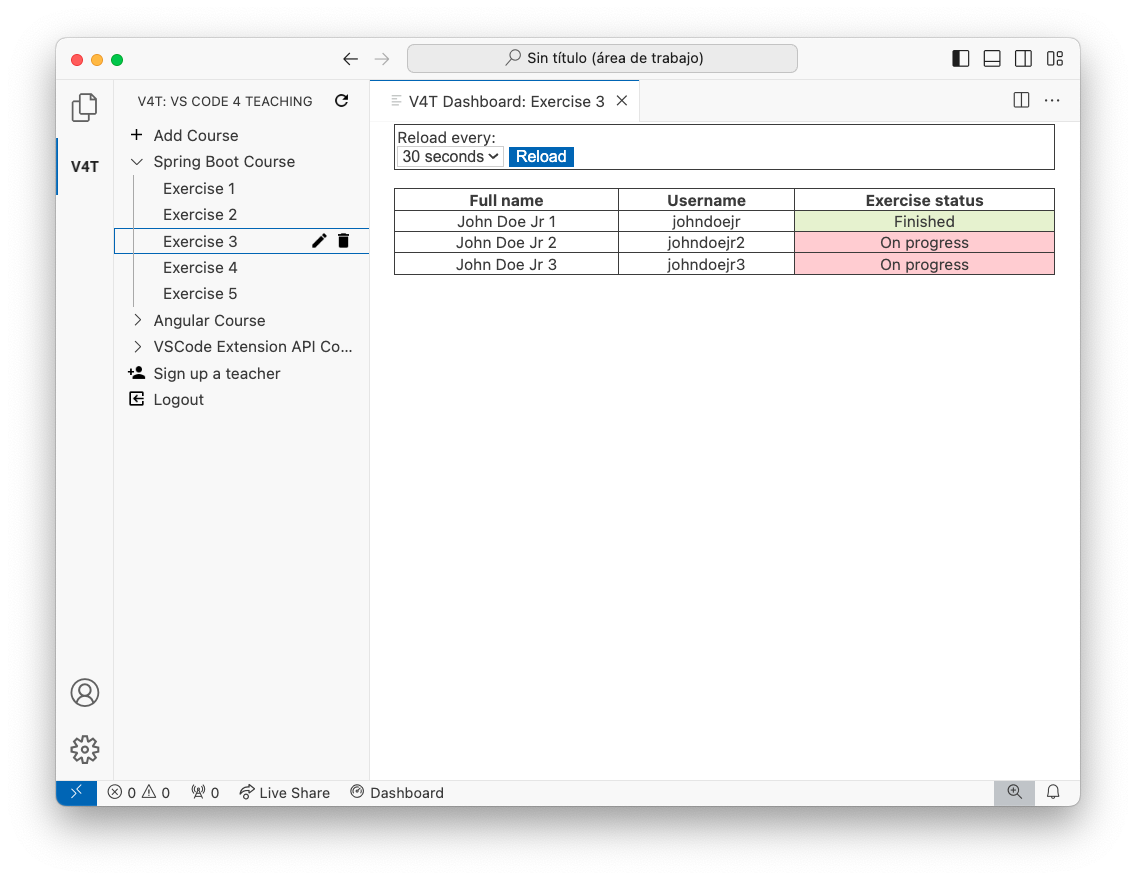
\includegraphics[width=0.825\linewidth]{imagenes/utilizadas/1-introduccion/historia-tfg1-dashboard.png}
    \caption{Captura del \textit{dashboard} para el seguimiento del progreso de los ejercicios en el primer TFG.}
    \label{fig:historiaProyecto1Dashboard}
\end{figure}

\begin{figure}[ht!]
    \centering
    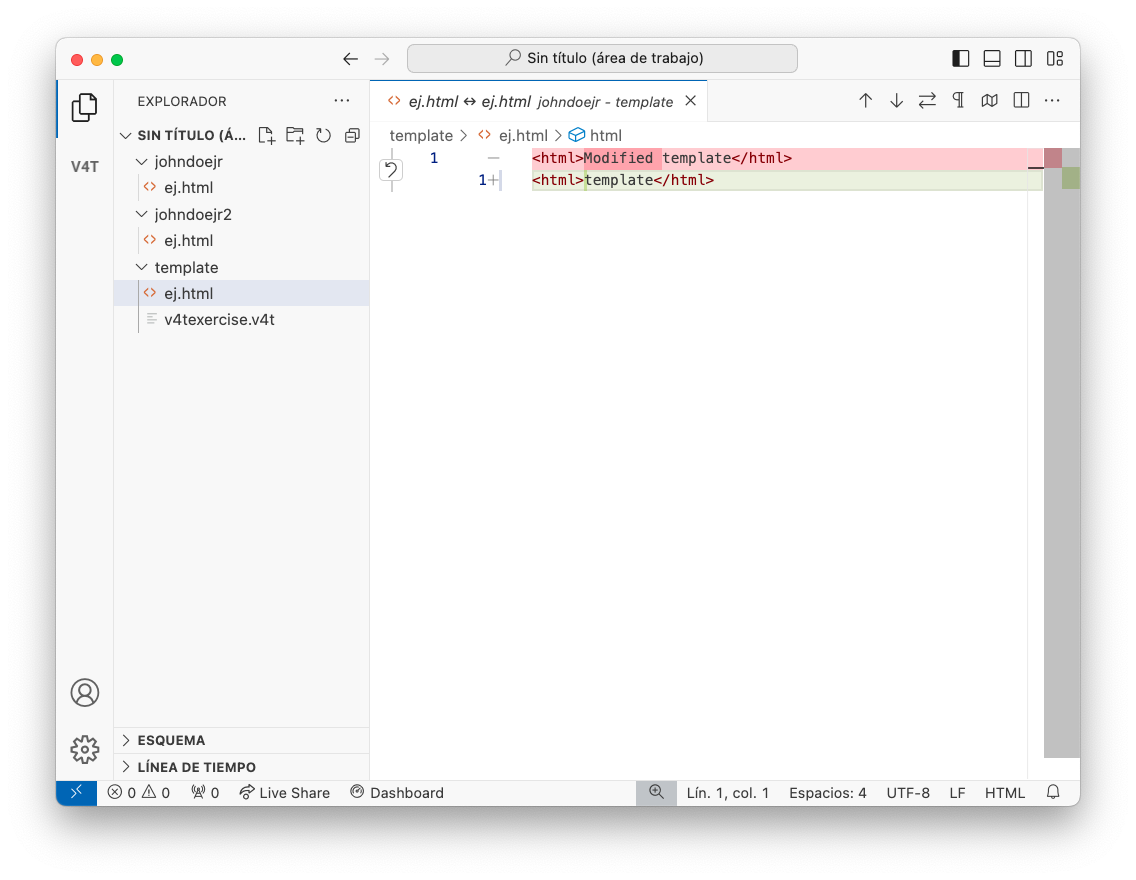
\includegraphics[width=0.825\textwidth]{imagenes/utilizadas/1-introduccion/historia-tfg1-comparacionFicheros.png}
    \caption{Captura de la capacidad para comparación de ficheros en \textit{VSCode4Teaching} en el primer TFG.}
    \label{fig:historiaProyecto1Comparacion}
\end{figure}


El \textbf{segundo} peldaño en la ``escalera'' evolutiva del proyecto \textit{VSCode4Teaching} se produce durante el Trabajo Fin de Grado de Álvaro Justo Rivas Alcobendas \cite{TFG_Alvaro}. Esta contribución potencia la usabilidad de la herramienta, incorporando numerosas características para lograr una experiencia de usuario más completa y que proporcione mejor información sobre todos los procesos de negocio realizados. A este respecto, destaca la incorporación de la actualización en tiempo real del \textit{dashboard} de los docentes y una mejora en su apariencia y funcionalidad, dotándolo de un nuevo estado para los ejercicios ``en progreso'' y de botones para facilitar el acceso a la visualización de los ficheros que componen las propuestas de los estudiantes y sus diferencias respecto a la plantilla original, tal como se refleja en la \referenciaFigura{fig:historiaProyecto2Dashboard}.

\begin{figure}[ht!]
    \centering
    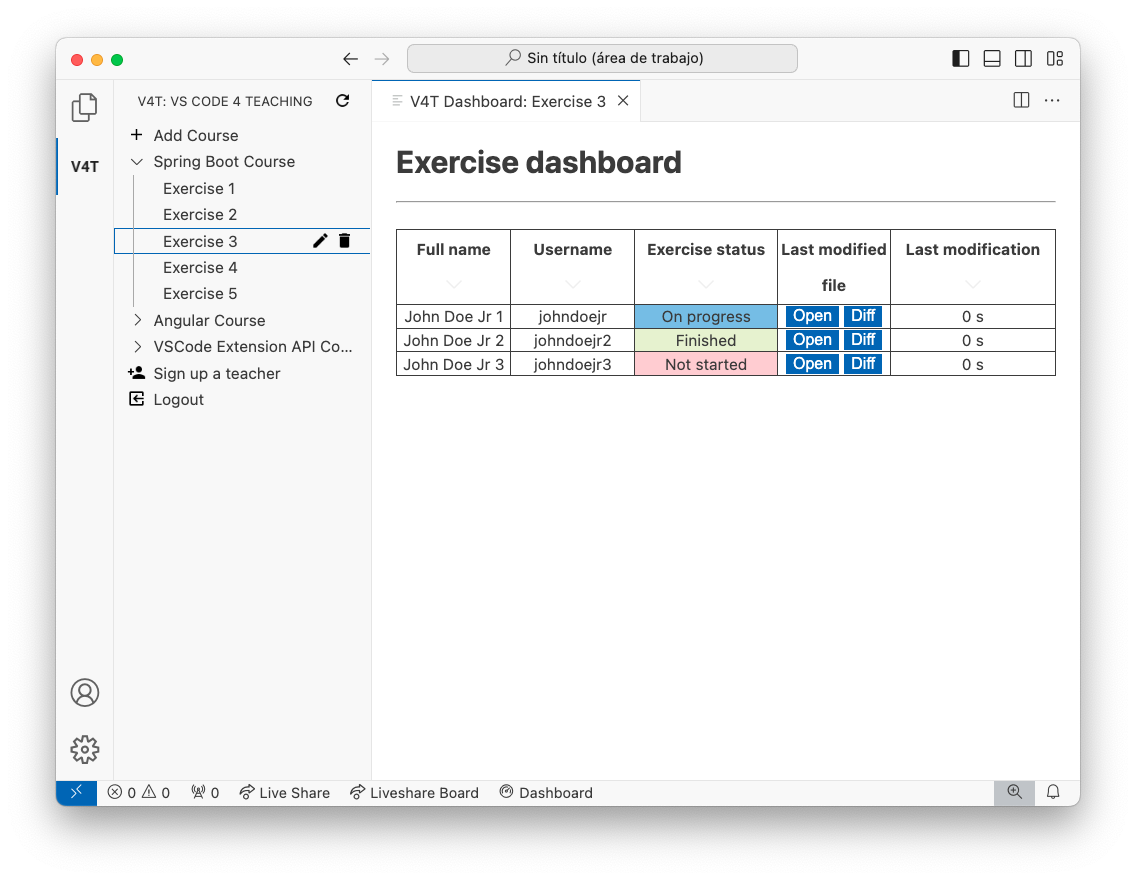
\includegraphics[width=0.825\textwidth]{imagenes/utilizadas/1-introduccion/historia-tfg2-dashboard.png}
    \caption{Captura del \textit{dashboard} para el seguimiento del progreso de los ejercicios en el segundo TFG.}
    \label{fig:historiaProyecto2Dashboard}
\end{figure}

El \textbf{tercer} hito evolutivo del proyecto quedó materializado a través del TFG de Diego Guerrero Carrasco \cite{TFG_Diego1} (autor del presente Trabajo Fin de Grado). Esta iteración añade nuevas funcionalidades, tales como la capacidad para poder añadir a cada ejercicio una propuesta de solución elaborada por el docente, de modo que los estudiantes puedan descargarla cuando el profesor decida hacerla pública y compararla con su propia propuesta de resolución del ejercicio a través de una herramienta gráfica. A esta mejora se suma, además, la capacidad para poder crear múltiples ejercicios a partir de los subdirectorios existentes en una carpeta, la preservación del anonimato de los estudiantes en el sistema de ficheros de la aplicación, de modo que solo el docente pueda relacionar a un alumno con su propuesta de resolución; un nuevo proceso para el alta de docentes basado en un formato de invitaciones entre pares y numerosas mejoras en materia de usabilidad: un menú contextual disponible en los ejercicios y nuevos iconos para mostrar a golpe de vista el progreso en la ejecución de los ejercicios ---tal como refleja la \referenciaFigura{fig:historiaProyecto3GUI}---, una nueva página de ayuda personalizada para cada curso compartido, con información específica del profesor que expide y divulga el código, y un rediseño del \textit{dashboard} para hacerlo más visual e intuitivo ---capturado en la \referenciaFigura{fig:historiaProyecto3Dashboard}---, añadiendo un nuevo gráfico del progreso de los estudiantes y otras métricas numéricas de utilidad sobre el ejercicio. En su faceta técnica, se añade durante esta fase, además, un nuevo componente al proyecto: una aplicación web que sirve como soporte para la implementación de algunas funcionalidades y que actúa de cliente en el modelo cliente-servidor descrito anteriormente.

\begin{figure}[ht!]
    \centering
    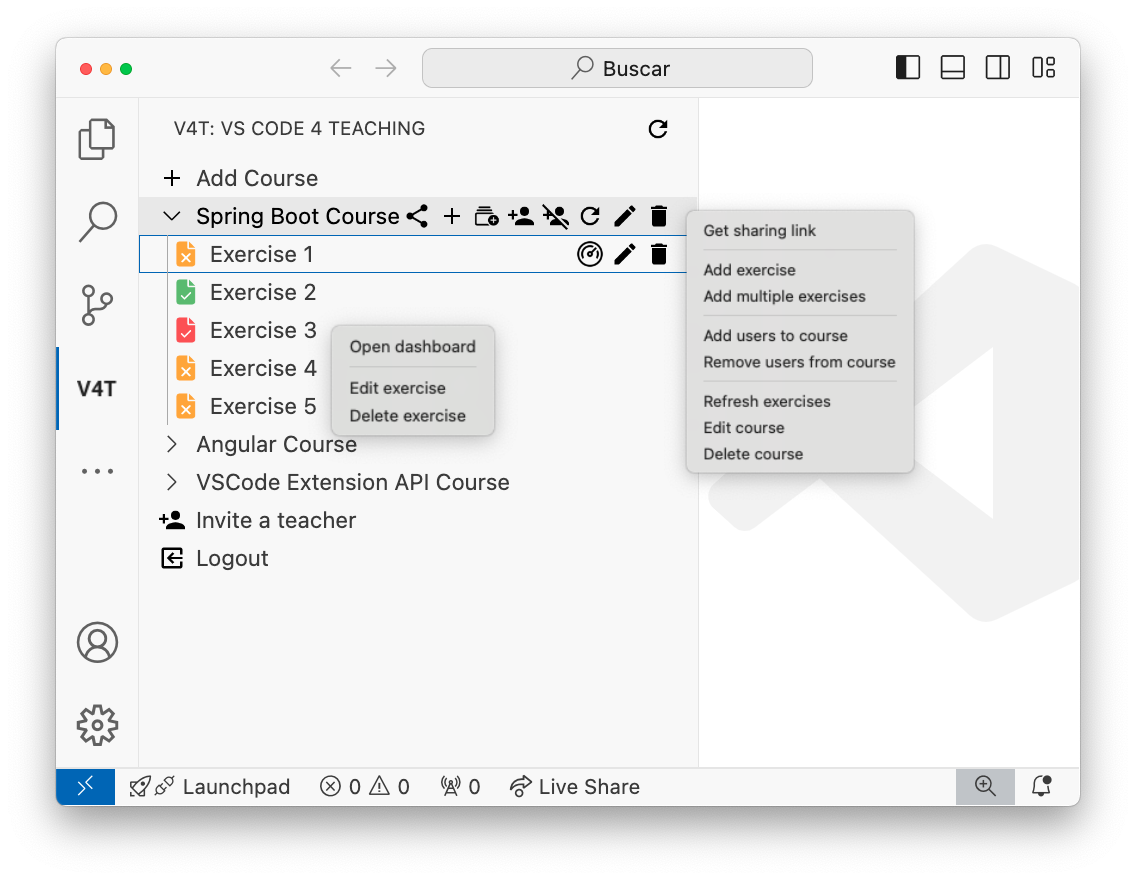
\includegraphics[width=0.825\textwidth]{imagenes/utilizadas/1-introduccion/historia-tfg3-gui.png}
    \caption{Captura de la barra lateral de la extensión con los nuevos iconos y menús contextuales.}
    \label{fig:historiaProyecto3GUI}
\end{figure}

\begin{figure}[ht!]
    \centering
    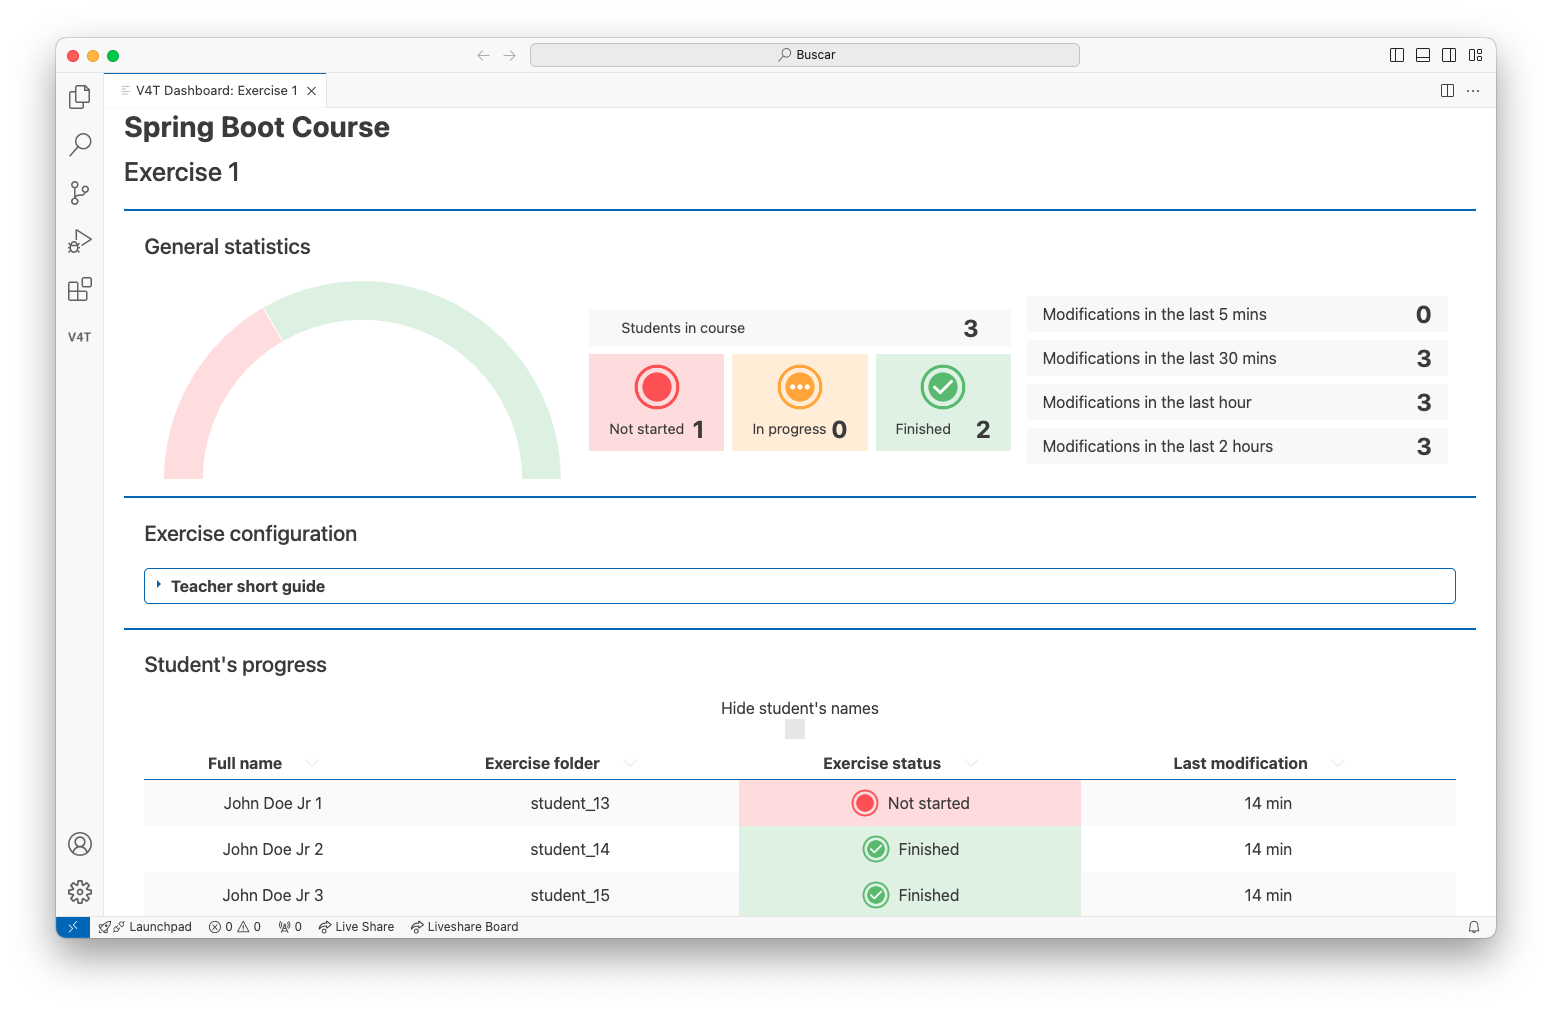
\includegraphics[width=\textwidth]{imagenes/utilizadas/1-introduccion/historia-tfg3-dashboard.png}
    \caption{Captura del \textit{dashboard} para el seguimiento del progreso de los ejercicios en el tercer TFG.}
    \label{fig:historiaProyecto3Dashboard}
\end{figure}

\section{Contexto técnico y motivación}
\label{sec:contxtTecnico}
Una vez planteado el contexto en el que surge la necesidad general del proyecto \textit{VSCode4Teaching} en la \referenciaSeccion{sec:contxtSocial}, y establecido qué es, cómo funciona y cómo se ha construido en la \referenciaSeccion{sec:cronologiaProyecto}, se justifica a continuación la motivación que conduce a realizar el presente Trabajo Fin de Grado.

\textit{VSCode4Teaching} es una aplicación que los usuarios únicamente pueden utilizar a través de un solo IDE\footnote{IDE. Siglas de ``entorno de desarrollo integrado'' (del inglés \textit{Integrated Development Environment}).}: Visual Studio Code.

A este respecto, la \textit{Encuesta sobre el estado de los desarrolladores}, realizada anualmente por JetBrains, recoge en su edición de 2023 \cite{JetBrains_DevState} las respuestas de $26\ 348$ encuestados acerca del uso de distintas tecnologías y herramientas durante el ejercicio de su profesión. De entre ellos, cabe poner el foco en el $19,7\%$ ($5190$) que afirman ser estudiantes de programación. Los datos recogidos para este grupo se incluyen en la \referenciaTabla{tab:usoIDEs}, que refleja las tasas de utilización y preferencia para varios entornos de desarrollo.

\begin{table}
    \caption{Uso de los entornos de desarrollo más populares entre los estudiantes.}
    \label{tab:usoIDEs}
    \centering
    \begin{tabular}{|c|c|c|c|c|}
        \multirow{2}{*}{\textbf{Entorno}} & \multicolumn{2}{c|}{\makecell{\scriptsize Usuarios que lo\\ \textbf{utilizan}}} & \multicolumn{2}{c|}{\makecell{\scriptsize Usuarios que lo\\ \textbf{prefieren}}} \\
        \cline{2-5}
                                          & \textbf{Nº} & \textbf{\%} & \textbf{Nº} & \textbf{\%} \\
        \hline
        Visual Studio Code                & 3512        & 67,67 \%    & 1401        & 26,99 \%    \\
        \hline
        IntelliJ IDEA                     & 2442        & 47,05 \%    & 965         & 18,59 \%    \\
        \hline
        PyCharm                           & 1779        & 34,28 \%    & 424         & 8,17 \%     \\
        \hline
        Visual Studio                     & 1063        & 20,48 \%    & 239         & 4,61 \%     \\
        \hline
        Android Studio                    & 953         & 18,36 \%    & 145         & 2,79 \%     \\
        \hline
        CLion                             & 806         & 15,53 \%    & 164         & 3,16 \%     \\
        \hline
        Vim                               & 745         & 14,35 \%    & 87          & 1,68 \%     \\
        \hline
        WebStorm                          & 725         & 13,97 \%    & 144         & 2,77 \%     \\
        \hline
        Notepad++                         & 595         & 11,46 \%    & 24          & 0,46 \%     \\
        \hline
        \hline
        Total                             & 5190        &             &             &             \\
        \hline
    \end{tabular}
    \\
    {\footnotesize \textbf{Nota:} datos porcentuales respecto al total de estudiantes encuestados.}
\end{table}


Entre los estudiantes destaca Visual Studio Code, siendo un entorno empleado por casi siete de cada diez estudiantes, aunque es el preferido por solo el $27\%$ de este grupo. Sin embargo, la tabla permite constatar que existe un amplio espectro de estudiantes que prefieren utilizar otras opciones, sobresaliendo IntelliJ IDEA y PyCharm, entornos de desarrollo de la empresa JetBrains dedicados a la creación de proyectos sobre las plataformas Java y Python, respectivamente.

Aunque un $67,67\%$ del público objetivo es un porcentaje adecuado, la tasa de estudiantes que afirman preferir Visual Studio Code es sensiblemente inferior, existiendo una gran heterogeneidad en la preferencia por los distintos entornos de desarrollo. De este modo, cabe poner sobre la mesa la posibilidad de ampliar el alcance del proyecto \textit{VSCode4Teaching}, tratando de llegar a la máxima cantidad de usuarios posible. La única alternativa que permitiría alcanzarlo es ofrecer la posibilidad de utilizar la aplicación fuera de Visual Studio Code.

Planteado este escenario, surgen diversas alternativas a ponderar para aumentar el alcance del proyecto. Una de ellas podría ser, por ejemplo, desarrollar una extensión paralela compatible con los entornos de JetBrains, que suman entre todos ellos ---IntelliJ IDEA, PyCharm, CLion y WebStorm en la clasificación anterior--- un $32,69\%$ de preferencia por el estudiantado encuestado. Sin embargo, tal como refleja la documentación de JetBrains al respecto \cite{JetBrains_Plugins}, el conjunto de tecnologías empleado para ello es notablemente diferente del que utiliza la extensión para Visual Studio Code, ya que requieren utilizar Kotlin como lenguaje de programación y Gradle para la gestión de la configuración del \textit{software}, hecho que dificultaría el mantenimiento del proyecto \textit{software} al añadir un componente nuevo que, además, requiere formas de mantenimiento diferentes de los demás y, por otro lado, la cota de público objetivo alcanzado aumenta hasta el $59,69\%$ de usuarios, que es una cifra elevada pero no lo suficientemente como para ejecutar este planteamiento.

Por tanto, la decisión es generar un nuevo cliente distinto de la extensión para Visual Studio Code que se base en una plataforma que sea independiente del IDE que empleen estudiantes o profesores. Generar una aplicación de escritorio conduciría a la misma conclusión que la extrapolada al inicio de este planteamiento, y es que cada usuario puede estar empleando un sistema operativo distinto, hecho que exige la construcción de varias aplicaciones que permitan utilizar \textit{VSCode4Teaching}. Por tanto, de nuevo, la opción de trasladar la funcionalidad a una aplicación de escritorio queda descartada por su complejidad técnica y la dificultad para su mantenimiento.

Con esta motivación y tras el análisis de las opciones disponibles, surge la idea de desarrollar una aplicación web que permita realizar todos los procesos de negocio que \textit{VSCode4Teaching} ya tiene implementados a través de una interfaz. De este modo, los usuarios podrían emplear el entorno de desarrollo y el sistema operativo de su preferencia, dependiendo únicamente del uso de un navegador web actual para garantizar que el proceso más relevante, que es la sincronización bidireccional de ficheros ubicados en el sistema local de los usuarios, puede realizarse correctamente.

\section{Estructura del documento}
\label{sec:estructura}
El presente documento describe detalladamente todos los trabajos realizados sobre el proyecto \textit{VSCode4Teaching} en su cuarto hito evolutivo.

El siguiente apartado (\referenciaCapitulo{cap:objetivos}) establece los objetivos que se buscará satisfacer mediante la realización del Trabajo Fin de Grado.

El tercer punto (\referenciaCapitulo{cap:tecnolHerramMetodo}) recoge el abanico de tecnologías y herramientas empleadas para la ejecución del trabajo, así como la metodología empleada y la organización para su realización.

El apartado cuarto (\referenciaCapitulo{cap:descInformatica}) incluye toda la descripción informática del trabajo ejecutado. Cabe reseñar que la aplicación queda compuesta por tres grandes componentes: el servidor, la extensión para Visual Studio Code y la aplicación web para navegadores, siendo este último el componente sobre el que se implementarán la práctica totalidad de los objetivos y requisitos.

Para finalizar, el capítulo quinto (\referenciaCapitulo{cap:conclusiones}) extrapola conclusiones tras finalizar el desarrollo, analizando la completitud de las necesidades establecidas y analizando trabajos futuros tentativos a realizar en sucesivas iteraciones.

A continuación, una vez finalizado el cuerpo del documento, se introduce la enumeración completa de las referencias bibliográficas a las que aluden las citas introducidas durante el desarrollo del documento.

\noindent\textbf{Nota:} este documento contiene numerosos enlaces e hipervínculos a otras secciones y epígrafes del documento, así como a las referencias bibliográficas, quedando escritos en {\color{RedLink}color rojo}. En su edición electrónica, el lector puede hacer \textit{click} sobre estos enlaces para ser conducido al punto al que referencian.




% Sección 2: Objetivos

% 1 página describiendo los objetivos concretos que se pretenden conseguir con el desarrollo del proyecto.
% Es como la conclusión de la introducción y la motivación capítulo anterior.
% \afterpage{\blankpage}
\chapter{Objetivos}
\label{cap:objetivos}

El \referenciaCapitulo{cap:introduccion} ha introducido pormenorizadamente la contextualización sociocultural que constata la necesidad del proyecto \textit{VSCode4Teaching}, una cronología de las distintas evoluciones que lo han ido conformando y la necesidad de generar una nueva interfaz para que los usuarios puedan utilizar esta herramienta sin necesidad de hacer uso de Visual Studio Code.

El presente Trabajo Fin de Grado busca alcanzar el cuarto hito en la evolución del proyecto, poniendo el foco en la necesidad anteriormente descrita con el fin de alcanzar a la mayor cantidad de potenciales usuarios posible, facilitando el acceso y la utilización de la herramienta. Esta necesidad es la piedra angular de este Trabajo Fin de Grado, que fija como su objetivo principal alcanzar al mayor público objetivo posible.

Traducido al plano técnico, este objetivo se va a materializar a través de la \textbf{implementación de un componente nuevo} en \textit{VSCode4Teaching}: una aplicación web que actúe como cliente (esto es, un \textit{frontend}), recogiendo toda la funcionalidad posible de la extensión y haciéndola independiente de Visual Studio Code, desapareciendo así el único requisito \textit{software} que se imponía a los usuarios. De este modo, la nueva aplicación web permitirá a sus usuarios ejecutar todos aquellos procesos de negocio que venían pudiendo realizar en la extensión para Visual Studio Code y que no dependiesen específicamente del citado entorno de desarrollo. Este matiz conduce a la exclusión de características como, por ejemplo, la capacidad para introducir comentarios textuales asociados a las líneas de código de los ficheros, característica intrínsecamente vinculada al entorno de desarrollo.

El proyecto ya dispone de una pequeña aplicación web implementada mediante Angular que se emplea como componente auxiliar para la ejecución de funcionalidades como el registro en dos partes de nuevos docentes mediante invitación y la visualización de una página de ayuda personalizada para alumnos cuando reciben una invitación a un curso por parte de un profesor. Como el alcance pretendido es más amplio y se dirige a la obtención de un componente renovado y completo, el objetivo principal de este Trabajo Fin de Grado en el plano técnico es el de generar una nueva aplicación web desde cero que permita alcanzar el objetivo de dominio, reemplazando el anterior \textit{frontend} existente.

Por todo lo anterior, cabe concluir que esta nueva evolución del proyecto \textit{VSCode4Teaching} busca acoplar al proyecto una aplicación web de lado cliente que permita a estudiantes y profesores operar con sus cursos y ejercicios, pudiendo ejecutar todos los procesos de negocio posibles de los previamente existentes. Este hecho conduce a que objetivos de dominio de este Trabajo Fin de Grado se fundamenten en los objetivos de negocio establecidos en las tres iteraciones previas, entre los que cabe destacar los siguientes seis objetivos:
\begin{enumerate}
    \item \underline{Autenticación y visualización personalizada de cursos y ejercicios}: permitir a los usuarios autenticarse, de modo que cada usuario podrá visualizar sus cursos inscritos o impartidos y los ejercicios que los compongan.
    \item \underline{Impartición de cursos y ejercicios por docentes}: brindar a los docentes las herramientas para gestionar sus cursos y añadir en ellos ejercicios a partir de plantillas iniciales y, opcionalmente, incorporándoles propuestas de solución que estarán disponibles al estudiantado cuando el docente lo desee.
    \item \underline{Seguimiento activo de ejercicios para docentes}: dotar a los docentes de las herramientas necesarias para seguir el progreso de los estudiantes al realizar los ejercicios de sus cursos, obteniendo información actualizada en tiempo real y pudiendo descargar sus propuestas de resolución.
    \item \underline{Matriculación del estudiantado en cursos}: permitir a los docentes gestionar los estudiantes que están matriculados en sus cursos y, además, compartirlos para permitir a los estudiantes automatricularse en ellos.
    \item \underline{Realización de ejercicios en cursos matriculados por alumnos}: otorgar a los estudiantes la capacidad para descargar los ficheros asociados a los ejercicios de los cursos de los que forman parte para realizarlos, sincronizando las modificaciones que vayan realizando según se produzcan.
    \item \underline{Calidad del proyecto y de su \textit{software}}: realizar actuaciones para mantener y mejorar el propio proyecto \textit{software}, migrando y ampliando el sistema de integración continua y, además, mejorando y automatizando la generación de los artefactos compilados de la aplicación para adecuar su despliegue y distribución al nuevo componente introducido.
\end{enumerate}


% Sección 3: Tecnologías, Herramientas y Metodologías

% Descripción de los lenguajes de programación, entornos de desarrollo, herramientas auxiliares, librerías de
% terceros, sistemas operativos, navegadores web, etc... utilizados para la realización del proyecto así como la
% metodología empleada. El grado de profundidad a la hora de explicar cada tecnología dependerá de lo relevante que
% ha sido para el proyecto y lo conocida que es. Por ejemplo, si se usa el lenguaje de programación Java, no es
% necesario entrar en tanto detalle que si se usa un lenguaje mucho menos usado como Scala, por ejemplo. Respecto
% a la metodología, dada la naturaleza de los proyectos, se suele describir una metodología iterativa e incremental
% en espiral, en la que se van sucediendo reuniones con el profesor que van definiendo el ámbito del proyecto.
% Este capítulo puede tener una extensión entre 10 y 15 páginas.
% \afterpage{\blankpage}
\chapter{Tecnologías, herramientas y metodología}
\label{cap:tecnolHerramMetodo}

Se presenta a continuación la diversidad de tecnologías (\referenciaSeccion{sec:tecnologias}) y herramientas (\referenciaSeccion{sec:herramientas}) involucradas en el proyecto \textit{VSCode4Teaching}, así como la metodología de trabajo empleada (\referenciaSeccion{sec:metodologia}) para realizar el presente trabajo.

\section{Tecnologías}
\label{sec:tecnologias}

Esta sección recoge información acerca de las tecnologías empleadas en el proyecto \textit{VSCode4Teaching}, describiéndolas en subsiguientes secciones dispuestas para cada uno de los componentes del proyecto (al respecto de los componentes y su arquitectura, véase la \referenciaSeccion{sec:diseñoArquitectura}): la aplicación web (\referenciaSeccion{subsec:tecAppWeb}), que toma el papel protagonista en el presente hito evolutivo, la extensión para Visual Studio Code (\referenciaSeccion{subsec:tecExtension}) y el servidor (\referenciaSeccion{subsec:tecServidor}). A estas secciones se añade, además, una sección adicional acerca de las tecnologías para la divulgación del código de la herramienta y su distribución y despliegue (\referenciaSeccion{subsec:tecDivulgDistribDeploy}).

\subsection{Aplicación web}
\label{subsec:tecAppWeb}

La nueva aplicación web de \textit{VSCode4Teaching} se basa en \textbf{Angular}, que emplea \textbf{Node} como plataforma subyacente, que se implementa utilizando el lenguaje \textbf{TypeScript} y que hace uso de bibliotecas para la comunicación con el servidor (\textbf{RxJS}), para la interacción con el sistema local de ficheros (mediante la \textbf{File System Access API}) y para la mejora de la \textbf{interfaz de usuario}.

\subsubsection{Angular}
\label{subsec:tecAngular}
Angular es un ``\textit{framework}\footnote{\textit{Framework}. Del inglés ``marco de trabajo'', es un conjunto de conceptos, prácticas y estándares que facilitan la consecución de un determinado objetivo, como la creación de aplicaciones o la gestión de un proceso \textit{software}.} web que facilita a los desarrolladores la creación de aplicaciones rápidas y fiables''\cite{Tec_Angular}. Fue desarrollado y está activamente mantenido por una subdivisión de Google, es de código abierto divulgado bajo licencia MIT y permite la generación de aplicaciones web SPA\footnote{SPA. Siglas de ``aplicación de página única'' (del inglés \textit{Single Page Application}).} orientadas a componentes.

Las aplicaciones web SPA son aquellas que requieren una única obtención de sus contenidos básicos (su estructura declarada mediante HTML, sus hojas de estilo en formato CSS y sus \textit{scripts} implementados mediante JavaScript) en la primera petición efectuada, actualizando su interfaz durante la interacción de los usuarios ejecutando peticiones en segundo plano y actualizando en consecuencia el DOM\footnote{DOM. Siglas de ``modelo de objetos del documento'' (del inglés \textit{Document Object Model}). Es uno de los objetos principales en el contexto de un navegador web y contiene una estructura arborescente mutable y navegable que representa los elementos dispuestos en la interfaz de una web y se genera a partir del código HTML recibido.}. Este tipo de aplicaciones aporta ventajas en materia de rendimiento, ya que en la primera petición se devuelve todo el código y los \textit{scripts} necesarios, soliendo ser más costosa en tiempo y memoria, mejorando así la experiencia de usuario en las sucesivas interacciones dentro de la propia aplicación \cite{SPA_Ventajas}.

Otra de las principales características que suele acompañar al desarrollo de aplicaciones web SPA es su orientación a componentes. Por ejemplo, Angular define el concepto de componente como ``el bloque fundamental para la creación de aplicaciones'' \cite{Angular_Componentes}. Este \textit{framework} fundamenta su arquitectura en la disposición de los componentes y las interrelaciones que establecen entre sí. Tal ha sido su popularización por parte de las bibliotecas de generación de aplicaciones SPA que este concepto está en vías de ser integrado en los estándares de HTML y JavaScript para su utilización sin necesidad de bibliotecas adicionales a través de los \textit{Web Components} \cite{WebComponents}, siendo compatibles aún solo con las versiones más modernas de los navegadores más populares.

Tras exponer las principales ventajas aportadas por las aplicaciones web SPA, cabe analizar el estado del arte a este respecto. Son tres las tecnologías más recurrentemente empleadas: React, Vue y Angular. La \textit{Encuesta de Desarrolladores} de Stack Overflow señala en su edición de 2023 que React es la tecnología para \textit{frontend} favorita para el $42,87\%$ de desarrolladores profesionales encuestados, frente a Angular ($19,89\%$) y Vue ($17,64\%$) \cite{subsec:tecAppAngularSurvey}.

Del citado artículo junto con otro que remarca las diferencias entre Angular y React \cite{AngularReact}, se extrapolan algunos puntos clave sobre las dos opciones más extendidas. Por un lado, Angular, aunque tiene una curva de aprendizaje más compleja, está bien mantenido y documentado, es escalable, favorece la modularidad y se basa en TypeScript; mientras que React mejora en rendimiento durante la renderización, es más fácil de aprender, únicamente se preocupa de la vista, requiriendo dependencias adicionales para dar soporte a las demás capas de la arquitectura; e introduce una sintaxis propia (JSX) para intercalar HTML y JavaScript.

Es necesario reseñar, además, una diferencia radical entre ellos: mientras que Angular es un \textit{framework} ``completo'' que impone ciertos conceptos y prácticas durante el ciclo de desarrollo y que toma el control de la aplicación en tiempo de ejecución, React es una ``biblioteca para interfaces de usuario web y nativas'' \cite{React} que requiere de la instalación de librerías adicionales para alcanzar una funcionalidad similar. Esta diferencia es fundamental, ya que permite a Angular brindar mecanismos como la inyección de dependencias, que facilita su aprendizaje a desarrolladores acostumbrados a la orientación a objetos, mientras que React utiliza objetos del ámbito global en el navegador para la compartición del estado entre componentes.

Al ser un \textit{framework}, Angular está ``opinionado'' (por traducción literal del inglés ``opinionated''); esto es, su uso viene marcadamente influenciado por las sugerencias que elaboran sus propios creadores para hacer las aplicaciones, pasando por la utilización de un determinado lenguaje ---TypeScript---, de una determinada arquitectura ---basada en componentes--- y de, en definitiva, un método recomendado pero no obligado para el desarrollo de proyectos.

El \textit{framework} utilizado en este proyecto es Angular. A todas las ventajas justificadas anteriores se suman, además, tres factores dependientes del contexto: es el \textit{framework} empleado en la asignatura de Desarrollo de Aplicaciones Web del Grado en Ingeniería del \textit{Software}, lo que facilita su posterior mantenimiento por otros autores en el contexto en el que se viene desarrollando este proyecto; ya se venía utilizando en \textit{VSCode4Teaching}, que ya contaba con una pequeña aplicación web basada en Angular como página de inicio y para la implementación del registro de nuevos profesores mediante invitación ---tal como se introduce en la \referenciaSeccion{sec:cronologiaProyecto}---; y su uso se basa en las mismas plataformas que la extensión para Visual Studio Code, que son TypeScript como lenguaje de programación y Node como plataforma subyacente, lo que hace que tenga una curva de aprendizaje compartida entre los dos componentes y, además, facilita la posibilidad de reutilización de código.

El ecosistema de Angular dispone de una amplia variedad de funcionalidades que se pueden emplear en estas aplicaciones, entre las que destacan: Angular CLI, una herramienta por línea de comandos que ayuda a los desarrolladores a generar \textit{scaffoldings}\footnote{\textit{Scaffolding}. Del inglés ``andamio'', alude al conjunto de ficheros que conforman una plantilla inicial sobre la que se asienta una nueva unidad \textit{software}.} de nuevas piezas \textit{software}, a actualizar la versión de las dependencias Angular añadidas o a ejecutar, compilar y desplegar las aplicaciones, entre otros; Angular Forms, que permite controlar integralmente el funcionamiento de los formularios, con métodos avanzados para la validación de las entradas y proporcionando \textit{two-way data binding} (es decir, la capacidad de cambiar el valor de variables a partir de la interfaz de usuario, y viceversa); o Angular Router, para hacer aplicaciones SPA con capacidad de establecer un sistema de enrutamiento virtual que permita diferenciar las distintas pantallas disponibles. Además de todas las citadas, que han sido utilizadas en la aplicación web, existen algunas más, como SSR, para habilitar \textit{Server-Side Rendering}, de modo que la vista se renderice en el servidor y el cliente la reciba preparada para inyectarla en el DOM; Material, que añade una amplia colección de componentes preparados para la interacción con los usuarios; o Localize, que facilita ofrecer una misma aplicación en múltiples idiomas.

Este proyecto utiliza Angular 16, publicado en mayo de 2023. Habitualmente, se libera una versión \textit{major}\footnote{\textit{Major}. En el sistema de versionado semántico\footnotemark, primera cifra en la nomenclatura de cada versión. Un salto de versión \textit{major} puede no ser retrocompatible.}\footnotetext{Versionado semántico. Sistema para la nomenclatura de nuevas versiones que se basa en la concatenación de tres secuencias numéricas: \textit{major}, \textit{minor} y \textit{patch}, ampliamente utilizado \cite{SemVer}.} nueva del \textit{framework} cada seis meses, hecho que dificulta mantener actualizados los proyectos a la última versión. Además, entre las versiones 16 y 17 se han producido numerosos cambios en el método de funcionamiento del \textit{framework}, por lo que se ha pospuesto la actualización a alguna versión más reciente.

\subsubsection{\textit{File System Access API}}
\label{subsec:tecFSA}
La \textit{File System Access API} (del inglés, ``interfaz para el acceso al sistema de ficheros'', y anteriormente llamada \textit{Native File System API}) es una interfaz proporcionada por algunos navegadores web para la interacción de las aplicaciones con el sistema de ficheros local de los usuarios.

Antes de entrar en detalle acerca de esta tecnología, cabe hacer un breve apunte acerca de la amplia variedad de navegadores web disponible y sus tendencias de uso. Según StatCounter \cite{UsoNavegadores}, los más utilizados en entornos de escritorio durante 2023 fueron Opera ($3,23\%$), Mozilla Firefox ($6,64\%$), Apple Safari ($8,8\%$), Microsoft Edge ($13,13\%$) y Google Chrome ($64,88\%$). Cada uno de estos navegadores ha sido creado y es mantenido por distintas corporaciones, hecho que ha conducido a una gran diversidad en los motores e intérpretes que utilizan. Los motores de renderizado son los componentes \textit{software} que los navegadores emplean para generar elementos gráficos a partir de la conjunción de la estructura definida mediante HTML y las hojas de estilo declaradas en CSS, siendo los más destacados \textit{WebKit} en el caso de Safari \cite{WebKit}, \textit{Gecko} en Firefox \cite{Gecko} y \textit{Blink} en los navegadores basados en Chromium \cite{Chromium}, Chrome y Edge \cite{Blink,EdgeChromium}. Por otro lado, los intérpretes de JavaScript, empleados para leer el código de los \textit{scripts} y ejecutarlo, son también diferentes para cada navegador, destacando \textit{SpiderMonkey} para Firefox \cite{SpiderMonkey} y \textit{V8} en el caso de Chrome y Edge \cite{V8}. Como resultado de esta heterogeneidad, se hace necesario revisar la compatibilidad de los \textit{scripts} implementados con las opciones disponibles en cada navegador, ya que un mismo código puede funcionar de forma diferente según el intérprete que lo ejecute.

La \textit{File System Access API} sienta sobre su base sobre la \textit{File System API} \cite{FileSystemAPI}, que es un ``estándar vivo'' de WHATWG (siglas de \textit{Web Hypertext Application Technology Working Group}), una comunidad integrada por desarrolladores encargados de actualizar muy frecuentemente varios estándares, entre los que destaca el que define HTML, promovida por grandes compañías de la informática como Apple, Mozilla Foundation u Opera. Este estándar define una interfaz para operar con sistemas de ficheros desde las aplicaciones web ejecutadas en el navegador a través de \textit{scripts}, estableciendo los métodos disponibles en los manejadores de ficheros (\textit{FileSystemFileHandle}) o directorios (\textit{FileSystemDirectoryHandle}) y en el BOM\footnote{BOM. Siglas de ``modelo de objetos del navegador'' (del inglés \textit{Browser Object Model}). Es el conjunto de objetos ofrecidos por el intérprete de un navegador, habitualmente designado como \texttt{window}, ya que suele ceñirse al contexto de una ventana o pestaña. Dentro de él se encuentra el DOM y permite ejecutar todas las operaciones accesibles del intérprete de \textit{JavaScript}, por lo que su funcionalidad depende del navegador empleado.}, tales como \textit{window.showOpenFilePicker}, para mostrar un diálogo que permita al usuario elegir un fichero en su sistema de ficheros local y dotar al navegador de un manejador del fichero basado en su contenido y metadatos; o \textit{window.showDirectoryFilePicker}, análogo para los directorios y sus contenidos; además de todos los métodos disponibles en las instancias concretas de las piezas \textit{software} que define este estándar.

Aunque esta API está parcialmente implementada en todos los navegadores, algunos de los más utilizados, como Firefox o Safari, restringen su uso a un sistema de ficheros privado y encapsulado localizado dentro del navegador llamado OPFS (siglas de ``sistema de ficheros de origen privado'', del inglés \textit{Origin Private File System}), accesible desde el BOM mediante el objeto \textit{navigator.storage}, de modo que estos navegadores no pueden operar con el sistema de ficheros local real del usuario que ejecuta una aplicación web que emplea esta API.

La \textit{File System Access API} propone complementar la \textit{File System API}. Esta API es actualmente un borrador divulgado por el WICG\footnote{WICG. Siglas de ``Grupo de la Comunidad para la Incubación de la Web'', del inglés \textit{Web Incubator Community Group}.}, que es un grupo dentro del W3C\footnote{W3C. Siglas de ``Consorcio Web'', del inglés \textit{World Wide Web Consortium}.} que sirve como ``lugar para la experimentación y discusión de nuevas características para la plataforma web'' \cite{WICG}. La propuesta de la \textit{File System Access API} tiene como propósito ``dotar a los desarrolladores de la capacidad para construir aplicaciones web que interactúen con ficheros en el dispositivo local del usuario [\dots], permitiendo modificar los archivos y trabajar con directorios'' \cite{FileSystemAccessAPI}. Para ello, propone la definición de los métodos \textit{queryPermission} y \textit{requestPermission}, que permiten solicitar permiso al usuario para ver o escribir (según se requiera) en el fichero o directorio que desee, dando como resultado una ampliación sobre las clases que ya proponía la \textit{File System API}. La definición de esta interfaz ampliada se preocupa de acotar los directorios que deben restringirse al implementarla en los navegadores, excluyendo los directorios críticos de los distintos sistemas operativos, aquellos que contienen el propio agente de usuario, la carpeta del usuario en sí misma y los directorios por defecto para el escritorio, los documentos o las descargas del usuario, entre otras.

Al no estar estandarizada, la compatibilidad de esta API queda restringida a cuantos navegadores la implementen. Los desarrolladores de Chrome son impulsores del uso de esta interfaz, lo que hizo que este navegador fuese el primero que dispusiese de ella, incorporándola en octubre de 2020. Además, publicaron un artículo divulgativo sobre ella en la que describen varios usos interesantes de la API acompañados de \textit{snippets}\footnote{\textit{Snippet}. Traducido literalmente del inglés como ``retal'', es un pequeño fragmento de código.} de código \cite{ArticuloChromeFsaAPI}: lectura y escritura de ficheros, especificación para guardar ficheros en local con sugerencia de nombre y ubicación, manejo de permisos concedidos por el usuario para acceder a un directorio, listado de contenidos de un directorio, creación o exploración de ficheros y directorios dentro de directorios, resolución de ruta relativa de ficheros localizados en directorios, renombrado, reubicación o eliminación de ficheros o directorios, integración con \textit{drag and drop}\footnote{\textit{Drag and drop}. Del inglés ``arrastrar y soltar'', se refiere a la capacidad para poder seleccionar uno o varios ficheros o directorios y arrastrarlos con el cursor hasta un área habilitada para la recepción, en la que se suelta el cursor. Es una interacción de usuario sustituta de la capacidad para elegir ficheros o directorios en un diálogo específicamente dispuesto con ese fin.} y métodos para el acceso al OPFS. Este artículo, además, va acompañado de una implementación de un editor web de ficheros localizados en el sistema local que, divulgado públicamente bajo licencia Apache 2.0, sirve como base y ejemplo de uso de gran parte de la funcionalidad de esta API \cite{ChromeLabsEditor}.

La heterogeneidad existente en la implementación de las interfaces por parte de los distintos intérpretes de los navegadores y la restricción vigente en Firefox y Safari, que no implementan los métodos de la \textit{File System Access API}, hace que el principal proceso de negocio de este proyecto, que es el intercambio bidireccional de ficheros entre el servidor y el cliente de \textit{VSCode4Teaching} para sincronizar las propuestas de los estudiantes y las plantillas de los ejercicios del profesorado, esté vigente únicamente en los navegadores Chrome, Edge y Opera, sumando un alcance de un $81,24\%$ de usuarios, aunque la restricción se puede ver fácilmente paliada al cambiar de navegador.

Una forma de mitigar parcialmente los efectos adversos derivados de esta divergencia en el funcionamiento de los navegadores es el uso de \textit{polyfills}, que son ``fragmentos de código que proveen la tecnología que se esperaría que un navegador proporcionase nativamente'' \cite{Polyfill}. En la práctica, los \textit{polyfills} funcionan en tiempo de ejecución, y detectan si el intérprete del navegador que los ejecuta dispone de los métodos deseados y, si no es así, añade una implementación efímera al vuelo, ya que quedará eliminada al cambiar de página.

Esta característica de sustitución en tiempo de ejecución que proponen los \textit{polyfills} puede no ser adecuada si se producen incompatibilidades entre la especificación original y la sustitutiva, pudiendo producir errores inesperados o difíciles de controlar. Para solucionar este problema, surge el concepto de \textit{ponyfill} \cite{Ponyfill}, que comparte finalidad con el anterior pero, en lugar de añadir implementaciones en tiempo real sobre las clases que no dispongan de los elementos deseados, propone una implementación independiente invocada utilizando una llamada a un módulo distinto, una biblioteca, que, internamente, dispondrá de una implementación no acoplada al estándar que se buscaba complementar originalmente, evitando utilizar la API nativa no soportada en su totalidad para garantizar que, con independencia de si el navegador que ejecuta el \textit{ponyfill} disponía de la funcionalidad deseada, funcione adecuadamente a través del mecanismo sustitutivo.

La contribución de los redactores del artículo de Chrome Labs anteriormente citado \cite{ArticuloChromeFsaAPI} no solo se ciñe al editor de texto, sino que, conscientes de la limitación para utilizar la API en algunos navegadores, implementaron y divulgaron un \textit{ponyfill} llamado \textit{browser-fs-access} \cite{BrowserFSAccess}, en el que también se basa el editor de texto que publicaron como caso de uso \cite{ChromeLabsEditor}, que dispone de implementaciones alternativas de los métodos de la \textit{File System Access API} basados en la utilización de elementos HTML como campos de tipo fichero o enlaces destinados a la descarga de documentos.

Este proyecto utilizó este \textit{ponyfill} para la implementación del proceso de sincronización de ficheros de estudiantes con el servidor, tal como se detalla en la \referenciaSeccion{subsec:rf11}. Además, se aprovecha la capacidad de este \textit{ponyfill} para advertir a los usuarios que utilizan navegadores no compatibles con la \textit{File System Access API} para mostrar por pantalla una recomendación para que cambien de navegador a otro que sí disponga de ella, tal como se define en la \referenciaSeccion{subsec:rn4}.

\subsubsection{RxJS}
\label{subsec:tecRxJS}
La programación reactiva es un paradigma de programación situado dentro del declarativo que basa su funcionamiento en el procesamiento de eventos asíncronos y en los flujos de datos \cite{ReactiveProgramming}. Esta marcada presencia de la asincronía se asocia intrínsecamente a una ejecución de código no bloqueante, declarando qué acciones se desearán ejecutar en el momento en que se reciba un dato a través de un flujo. Una vez declarado, continúa la ejecución del código sin pausarlo, ejecutando las acciones especificadas en el momento de recibir algún dato nuevo y dándolo a conocer a aquellos elementos que estén interesados en obtener la información procesada para, a su vez, producir nuevos eventos o alimentar otros flujos de datos.

La anterior descripción permite vislumbrar la aplicación práctica de un patrón de diseño clásico: \textit{Observer} \cite{GammaObserver}, en el que un informante tiene constancia de un grupo de observadores que quedan inscritos para recibir notificaciones sobre la modificación de su estado para, como consecuencia, realizar acciones derivadas de estas alteraciones. La programación reactiva bautiza al informante como ``observable'', a los observadores como ``suscriptores''; y a la acción que realizan estos sobre los primeros, ``suscripción''.

RxJS es una biblioteca para JavaScript y TypeScript que permite ``componer programas asíncronos y basados en eventos mediante la utilización de secuencias observables'' \cite{RxJS}. Divulgada como \textit{software} libre bajo licencia Apache 2.0, es una de las implementaciones del proyecto \textit{ReactiveX}, que propone múltiples implementaciones para llevar la programación reactiva a distintas plataformas \textit{software} \cite{ReactiveX}. Así, RxJS pone a disposición de sus usuarios clases que modelan observables y suscriptores a través de suscripciones, además de una amplia variedad de operadores para poder generar nuevos observables o para fusionar, transformar, mezclar o gestionar errores en los flujos asíncronos producidos por observables.

El cliente HTTP de Angular, incorporado por defecto en el \textit{framework}, permite preparar peticiones utilizando los observables de RxJS. Un uso típico estas tecnologías combinadas se ilustra en el \referenciaCodigo{cod:reqHttpAngular}, en el que se emplea un operador RxJS para convertir la información entrante en la respuesta de la petición en forma de DTO\footnote{DTO. Siglas de ``objeto de transferencia de datos'', del inglés \textit{Data Transfer Object}. Es un objeto sencillo que emplea tipos primitivos y que se utiliza para facilitar la transferencia de información entre componentes \textit{software}.} a una instancia del modelo y, además, un operador que permite cerrar automáticamente el observable al recibir la última respuesta (que, en una petición HTTP habitual, será la primera), finalizando el flujo asíncrono y desuscribiendo a sus observadores tras transmitir la respuesta procesada. Además, este último operador permite ``aplanar'' el flujo de datos: dado que se sabe que habrá una sola respuesta, es posible devolver una promesa\footnote{Promesa. En JavaScript y TypeScript, un objeto declarado asíncrono que devolverá eventualmente un valor afirmativo (resolución) o negativo (rechazo). Es estándar en JavaScript desde 2015, por lo que existen facilidades sintácticas del lenguaje para su uso \cite{Promise}.}, lo que, dado que están estandarizadas desde ES6 \footnote{ES6. Acrónimo de \textit{ECMAScript 6}, estándar del lenguaje JavaScript publicado en 2015. Los estándares publicados por ECMA son los más extendidos y empleados para generar intérpretes de JavaScript \cite{ES6}.}, facilita la codificación posterior.

\begin{lstlisting}[language=TypeScript,caption={Ejemplo de petición HTTP con el cliente de Angular (dependencia inyectada) y un observable de RxJS.},label=cod:reqHttpAngular]
public constructor(private http: HttpService) {}

public getCourseById = (id: number): Promise<Course> =>
    lastValueFrom(this.http.get<CourseDTO>("/course/" + id.toString())
        .pipe(map((courseDTO: CourseDTO) => new Course(courseDTO)))
    );
\end{lstlisting}

Sin embargo, resulta interesante emplear el comportamiento estándar de un observable de RxJS ---es decir, sin convertirlo en una promesa---, por ejemplo, al utilizar una conexión mediante \textit{Web Sockets}. Este protocolo permite dejar una conexión abierta bidireccional entre emisor y receptor, de modo que un observable sirve como interfaz para la recepción de mensajes de un \textit{web socket}, procesando las entradas e informando en el momento de la recepción a los suscriptores existentes, quienes pueden efectuar las acciones programadas como respuesta a la ocurrencia del citado evento asíncrono.

\subsubsection{TypeScript}
\label{subsec:tecTS}
Según Microsoft, creadores e impulsores de este proyecto, TypeScript es un ``lenguaje fuertemente tipado que transpila a JavaScript, brindando a los desarrolladores mejores herramientas a cualquier escala'' \cite{TypeScript}. Divulgado como código abierto bajo licencia Apache, TypeScript es un lenguaje de programación con tipado fuerte que proporciona una envoltura alrededor de JavaScript, aportando las principales ventajas del uso de tipos, como la detección de errores en tiempo de compilación como consecuencia de un mal uso de las variables según sus tipos definidos. Su uso se basa en un transpilador\footnote{Transpilador. Tipo particular de compilador que genera código fuente en un lenguaje a partir de código fuente en otro lenguaje.}, \textit{tsc}, que convierte el código TypeScript en su correspondiente JavaScript.

De las tecnologías analizadas en la \referenciaSeccion{subsec:tecAngular}, Angular es el único \textit{framework} de aplicaciones web para cliente que emplea TypeScript como lenguaje recomendado para su utilización durante el desarrollo. El propio \textit{framework} está implementado con este lenguaje e incorpora \textit{per sé} todas las herramientas necesarias para generar JavaScript automáticamente durante los procesos de construcción o ejecución de la aplicación con el fin de favorecer el uso de este lenguaje.

\subsubsection{Node}
\label{subsec:node}
Node.js (habitualmente denominado ``Node'') es un ``entorno de ejecución de JavaScript gratuito, de código abierto y multiplataforma que permite crear servidores, aplicaciones web, herramientas para línea de comandos y scripts'' \cite{Node} que se basa en V8, el intérprete de JavaScript que emplean navegadores como Chrome o Edge.

Si bien la intención original del lenguaje JavaScript, sexto lenguaje más usado con una cuota de uso del $3,32\%$ según TIOBE \cite{TIOBE} en junio de 2024, era la de dotar de dinamismo a las aplicaciones web mediante \textit{scripts} ejecutados en los navegadores al cargar las páginas, sus prestaciones han aumentado y en la actualidad dispone de herramientas de forma nativa que permiten trabajar mediante eventos asíncronos de forma sencilla, facilitando la creación de aplicaciones fundamentadas en el intercambio de información por red. La finalidad de Node es la traslación de estas ventajas a la posibilidad de ejecutar aplicaciones basadas en este lenguaje directamente como procesos en el sistema operativo para generar aplicaciones de escritorio o herramientas por línea de comandos.

Este último es el caso de Angular. Como se introduce en la \referenciaSeccion{subsec:tecAngular}, este \textit{framework} dota al desarrollador de una herramienta por línea de comandos que permite, entre otros procesos, ejecutar la aplicación o compilarla, para lo que se basa en herramientas asentadas en la plataforma Node. Además, por ejemplo, la capacidad para incorporar \textit{server-side rendering} (SSR) hace uso de un pequeño proceso Node a instalar en el servidor que se encarga de la generación de las vistas renderizadas transmitidas al cliente.

Otra de las capacidades asociadas a los proyectos basados en la plataforma Node es la utilización de un gestor de dependencias instalado por defecto junto con la distribución habitual de Node, que es NPM (siglas de \textit{Node Package Manager}). Además de un gestor de dependencias, NPM dispone de un repositorio público impulsado por GitHub con una gran cantidad de módulos reutilizables para los proyectos Node \cite{npmjscom}. Este gestor de dependencias se basa en las declaraciones albergadas en el fichero \texttt{package.json} que existe en la raíz de los proyectos Node, instalando todas las dependencias declaradas y sus transitivas en el directorio \texttt{node\_modules}. En el \referenciaCodigo{cod:packageJsonAngular} se introduce un fragmento del fichero \texttt{package.json} de la aplicación web para Angular, en el que se observa la declaración de algunos atributos básicos, tales como el nombre o la versión, de algunos atajos para la ejecución de \textit{scripts} que permiten ejecutar la aplicación o construirla y la declaración de dependencias, tanto las requeridas en tiempo de ejecución (\texttt{dependencies}) como las únicamente requeridas para el desarrollo (\texttt{devDependencies}).

\begin{lstlisting}[language=JavaScript,caption={Fragmento del documento \texttt{package.json} de la aplicación web Angular.},label=cod:packageJsonAngular]
{
    "name": "vscode4teaching",
    "version": "3.0.0",
    "scripts": {
        "start": "ng serve",
        "build": "ng build",
        // ...
    },
    "dependencies": {
        "@angular/common": "^16.2.9",
        "@angular/core": "^16.2.9",
        "@angular/forms": "^16.2.9",
        "@angular/router": "^16.2.9",
        // ...
    },
    "devDependencies": {
        "@angular/cli": "~16.2.6",
        "typescript": "^5.1",
        // ...
    }
}
\end{lstlisting}

\subsubsection{Interfaz de usuario: SCSS, Bootstrap y Chart.js}
\label{subsec:tecGUI}
A todas las tecnologías desarrolladas durante las subsecciones anteriores, se añaden algunas otras bibliotecas y tecnologías empleadas para facilitar la generación de una interfaz de usuario visualmente atractiva, fácilmente operable e intuitiva. Para ello, se han empleado \textbf{SCSS} como preprocesador de hojas de estilo, \textbf{Bootstrap} como biblioteca para la disposición básica de los elementos y \textbf{Chart.js} como ejemplo de biblioteca para la generación de componentes visuales avanzados.

CSS (siglas en inglés de ``hojas de estilo en cascada'') es el lenguaje declarativo empleado de forma estándar para la definición de los estilos que se deben aplicar sobre la definición de la estructura de una visualización web a través de una maqueta en HTML. Este estándar es mantenido por un grupo de trabajo del W3C \cite{CSS_W3C}, y es aplicado por todos los motores de renderizado de los navegadores más empleados.

De una forma similar a como TypeScript envuelve JavaScript, alrededor de CSS surgió \textbf{Sass} (``hojas de estilo sintácticamente increíbles'', del inglés \textit{Syntactically Awesome Style Sheets}) \cite{Sass}, que introduce algunas características de las que CSS no disponía en sus versiones más antiguas, como el uso de variables, el anidamiento de selctores y reglas u operadores automáticos. Sass es de código libre, está divulgado bajo licencia MIT, y que ofrece dos sintaxis: SCSS, que emplea el mismo concepto sintáctico que CSS; o la sintaxis indentada, que elimina los caracteres de separación de ámbitos y reglas y los sustituye, respectivamente, por tabulaciones y saltos de línea. Proporciona un transpilador que permite generar el CSS compatible con los motores de renderizado.  

Angular ofrece soporte a la transpilación de Sass, incorporándola al proceso de ejecución y construcción de aplicaciones de forma automática, pudiendo configurar en los proyectos si harán uso de CSS o de alguna de las dos sintaxis que propone Sass. La aplicación web de \textit{VSCode4Teaching} define sus hojas de estilo haciendo uso de la sintaxis SCSS.

\textbf{Bootstrap} es un ``conjunto de herramientas para \textit{frontend} poderoso, extensible y empaquetado por características'' que ``está construido con Sass, utiliza un sistema de cuadrícula y aporta componentes a través de poderosas extensiones JavaScript'' \cite{Bootstrap} publicado como \textit{software} libre bajo licencia MIT. Ofrece una especificación de estilos básica para todos los elementos visuales, aportándoles una estética común, además de un conjunto de componentes funcionales JavaScript básicos, entre los que destacan las ventanas modales embebidas.

\textbf{Chart.js} es una biblioteca ``simple y flexible'' \cite{ChartJS} para generar gráficos de diversa índole a partir de una configuración básica y una serie de datos. Específicamente, se utiliza para generar un gráfico semicircular representativo del progreso de los estudiantes al realizar un ejercicio (véase la \referenciaSeccion{subsec:rf3}).

\subsection{Servidor}
\label{subsec:tecServidor}
Si bien este Trabajo Fin de Grado pone el foco en la generación del nuevo \textit{frontend} Angular (véase la \referenciaSeccion{subsec:tecAppWeb}), esto no es óbice para exponer a continuación las tecnologías empleadas para la generación del servidor, que es la base sobre la que funciona el conjunto del proyecto. Este servidor está implementado en \textbf{Spring Boot} (basado en el \textit{framework} Spring), hace uso de un sistema de persistencia materializado en una \textbf{base de datos MySQL}, potencia su funcionalidad mediante bibliotecas gestionadas con \textbf{Maven} e incorpora una batería de pruebas automáticas sobre la plataforma \textbf{JUnit}.

\subsubsection{Persistencia de la información: MySQL}
\label{subsec:tecMySQL}
\textit{VSCode4Teaching} asienta su lógica de negocio sobre un modelo del dominio que introduce varias entidades interrelacionadas, tal como queda reflejado en la \referenciaSeccion{subsec:arqDominio}. Para la persistencia de la información asociada a cada entidad y sus interconexiones, se hace uso de un sistema gestor de bases de datos (SGBD) de tipo relacional. En estos sistemas, cada base de datos contiene una colección de tablas, que son estructuras bidimensionales que almacenan tuplas (registros) de información estructurada en atributos (columnas) comunes a todas, permitiéndose el establecimiento de relaciones lógicas entre los atributos de distintas tablas para dar lugar a un conjunto de datos coherente en el dominio especificado.

Concretamente, el sistema gestor empleado para la persistencia de la información en el proyecto \textit{VSCode4Teaching} es MySQL. Este gestor es mantenido por Oracle Corporation y se divulga con licencia pública de GNU (GPL) en su versión \textit{Community}, abierta a su uso no comercial para la comunidad \cite{MySQL}. Según la \textit{Encuesta de Desarrolladores} realizada por Stack Overflow en su edición de 2023 \cite{subsec:tecAppAngularSurvey}, MySQL es el segundo sistema gestor de bases de datos más empleado, alcanzando una cuota de uso del $41,09\%$ según los más de $75\ 000$ encuestados, viéndose superado por primera vez por PostgreSQL, su principal alternativa, también \textit{software} libre divulgado bajo su propia licencia (PostgreSQL License, similar a la licencia MIT) \cite{PostgreSQL}, que alcanza una cuota de uso del $45,55\%$ y cuenta en la actualidad con un gran respaldo entre los desarrolladores profesionales.

\subsubsection{Java y Spring}
\label{subsec:tecSpring}
El servidor de \textit{VSCode4Teaching} es una aplicación basada en el \textit{framework} \textbf{Spring}, que hace uso de \textbf{Java} como plataforma para su implementación y ejecución.

\paragraph{Java}\mbox{} \\
Java es ``una plataforma informática de lenguaje de programación creada por Sun Microsystems en 1995'' \cite{Java}, actualmente parte de Oracle Corporation. Esta plataforma proporciona tres componentes principales: el propio lenguaje de programación, el entorno en tiempo de ejecución y las bibliotecas incorporadas por defecto.

El lenguaje de programación, también llamado Java, es uno de los más empleados en la actualidad, consolidado en la cuarta posición del índice TIOBE desde hace más de un año con una cuota de uso del $8,40\%$ (junio de 2024) \cite{TIOBE}. Es orientado a objetos y destaca por su tipado fuerte y el soporte a las características esenciales de este paradigma: abstracción, encapsulación, jerarquía, modularización, herencia, polimorfismo y genericidad.

La ejecución de programas implementados en este lenguaje requiere como paso intermedio la generación de \textit{bytecode}, que es un código objeto\footnote{Código objeto. Es un paso intermedio producido al compilar un código fuente y que puede ser interpretado mediante programas específicos.} apto para su posterior ejecución mediante el entorno en tiempo de ejecución de Java, \textit{Java Runtime Environment} (JRE), que basa su funcionamiento en la máquina virtual de Java (\textit{Java Virtual Machine} o JVM). Este formato de compilación a un código intermedio posteriormente interpretado en ejecución mediante un compilador JIT (\textit{just in time}) brinda a la plataforma Java una de sus capacidades más destacadas: la independencia del sistema operativo para la ejecución de las aplicaciones, ya que un mismo artefacto compilado puede ser ejecutado sobre cualquier JRE con independencia del sistema operativo en el que se generó.

A todas estas características se añade un tercer factor determinante: el conjunto de las bibliotecas incorporadas nativamente en Java, que proporcionan una gran cantidad de funcionalidad apta para todos los sistemas, permitiendo el acceso unificado a recursos para la gestión de la concurrencia, de las comunicaciones por red o de las interfaces gráficas de usuario, entre muchas otras.

\paragraph{Spring}\mbox{} \\
Spring es el \textit{framework} más empleado para la construcción de aplicaciones web basadas en la plataforma Java. Este dato está ratificado por la \textit{Encuesta de Desarrolladores} de Stack Overflow que, en su edición de 2023 \cite{subsec:tecAppAngularSurvey}, afirma que el $11,95\%$ de los encuestados utiliza Spring, siendo la duodécima tecnología web más empleada según la anterior clasificación, que aglutina una amplia variedad de tecnologías para el lado cliente, el lado servidor y algunos CMS\footnote{CMS. Siglas de ``sistema de gestión de contenidos'' (del inglés \textit{System Content Manager}). Habitualmente orientadas a la web, son aplicaciones que ponen a disposición de sus usuarios un conjunto de herramientas visuales que facilitan la generación de páginas y aplicaciones web con escasa o nula necesidad de implementación de código fuente.}.

Tal como introduce su propia información, Spring ``proporciona un modelo de configuración y programación fácilmente comprensible para crear aplicaciones modernas basadas en Java'' \cite{SpringFramework}. Este modelo está basado en el ecosistema alrededor del \textit{framework}: existe una ingente cantidad de bibliotecas que se pueden añadir a las aplicaciones basadas en Spring para introducirles funcionalidades adicionales de interés. Tanto Spring como todas sus dependencias son \textit{software} libre y se distribuyen en abierto bajo licencia Apache 2.0.

De entre todas las bibliotecas disponibles y empleadas para implementar el servidor, una de las más destacadas es \textbf{Spring Boot}, que facilita la utilización de Spring para ``crear fácilmente aplicaciones autocontenidas aptas para entornos de producción [\dots] que pueden simplemente ejecutarse'' \cite{SpringBoot}, ya que dispone de un servidor web embebido e introduce algunas dependencias de Spring por defecto para simplificar la configuración de la aplicación.

Otro proyecto del ecosistema Spring es \textbf{Spring Data}, que es un conjunto de bibliotecas que ``proporciona un modelo de acceso a datos familiar, consistente y basado en Spring que facilita el acceso a bases de datos relacionales y no relacionales'' \cite{SpringData} que, específicamente, es utilizado en el servidor para acceder a la base de datos MySQL empleada como sistema de persistencia de la información (véase la \referenciaSeccion{subsec:tecMySQL}), relegando los detalles de la comunicación y utilización de este sistema a un ORM\footnote{ORM. Siglas de ``mapeador objeto-relacional'' (del inglés \textit{Object Relational Mapper}). Es una pieza \textit{software} que permite interactuar con bases de datos mediante clases y objetos en el código con el fin de facilitar su uso.} que brinda la capacidad para la interacción bidireccional con la base de datos, encapsulando la necesidad de utilizar consultas y operaciones SQL para ello.

\subsubsection{Maven}
\label{subsec:tecMaven}
Los proyectos asentados sobre Java como plataforma tecnológica pueden hacer uso de Maven, que es un ``\textit{software} de gestión de proyectos basado en el concepto de un modelo de objetos de proyecto (\textit{Project Object Model} o POM) centralizado que permite manejar las distintas etapas de su ciclo de vida (construcción, ejecución, verificación\dots) y la generación de informes y documentación'' \cite{Maven}.

Creado por la \textit{Apache Software Foundation} y divulgado bajo licencia Apache 2.0, Maven permite gestionar proyectos mediante la centralización de su configuración en un único fichero, el POM (habitualmente llamado \texttt{pom.xml}), que está situado en la raíz de los proyectos Maven y recoge aspectos básicos de la definición del componente, tales como su nombre, licencia o autoría, además de características del \textit{software}, incluyendo la versión del componente, dependencias que emplea y otras configuraciones específicas para su compilación o ejecución.

Sirva como ejemplo el POM del servidor de \textit{VSCode4Teaching}, del que se incluye un fragmento en el \referenciaCodigo{cod:pomServidor}. Esta definición hace uso de algunos de los rasgos más importantes de la configuración mediante Maven: la declaración de la dependencia de Spring Boot como \texttt{parent} y de algunas de sus dependencias asociadas (\texttt{dependencies}), la declaración del nombre del artefacto generado y su versión, nombre y descripción y la versión de Java sobre la que se desarrolla (y, por tanto, la mínima requerida para su ejecución), entre otras configuraciones para su compilación y ejecución (\texttt{build}).

\begin{lstlisting}[language=XML,caption={Fragmento adaptado del fichero para la configuración de Maven aplicado en el servidor del proyecto (\texttt{pom.xml}).},label=cod:pomServidor]
<project [...]>
    <parent>
        <groupId>org.springframework.boot</groupId>
        <artifactId>spring-boot-starter-parent</artifactId>
        <version>2.7.16</version>
        <relativePath/>
    </parent>

    <groupId>com.vscode4teaching</groupId>
    <artifactId>vscode4teaching-server</artifactId>
    <version>2.2.1</version>

    <name>VSCode 4 Teaching</name>
    <description>Server side of VSCode 4 Teaching extension.</description>

    <properties>
        <java.version>11</java.version>
    </properties>

    <dependencies>
        <dependency>
            <groupId>org.springframework.boot</groupId>
            <artifactId>spring-boot-starter-data-jpa</artifactId>
        </dependency>
        <dependency>
            <groupId>org.springframework.boot</groupId>
            <artifactId>spring-boot-starter-web</artifactId>
        </dependency>
        [...]
    </dependencies>

    <build>
        [...]
    </build>
</project>
\end{lstlisting}

\subsubsection{JUnit}
\label{subsec:tecJUnit}
El servidor de \textit{VSCode4Teaching} cuenta con una batería de pruebas automáticas que permite su verificación y aseguramiento de su calidad, tal como se detalla en la \referenciaSeccion{subsec:testingServidor}. Estas pruebas se asientan sobre JUnit, que es una biblioteca muy extendida para la implementación y ejecución de pruebas o \textit{tests} en proyectos basados en la plataforma Java \cite{JUnit}. Fue creada por Kent Beck y Erich Gamma y se distribuye como código libre con licencia Eclipse Public License.

JUnit brinda a los desarrolladores la posibilidad de implementar pruebas basadas en aserciones ---esto es, comparaciones estrictas entre valores esperados y valores obtenidos tras la ejecución de las pruebas---, introduciendo soporte a la parametrización de pruebas (es decir, al uso de colecciones de distintos datos de prueba) y a los dobles, que son piezas \textit{software} que permiten reemplazar el comportamiento que tendrán ciertos componentes relacionados y utilizados en el SUT\footnote{SUT. Siglas de ``sujeto bajo pruebas'' (del inglés \textit{Subject Under Test}. Respecto a una prueba automática de \textit{software}, es la unidad del \textit{software} que el \textit{test} busca validar.)} que quedan verificados mediante otras pruebas. Es posible ejecutar la batería de pruebas manualmente mediante Maven y, además, se integra fácilmente con sistemas de integración continua, tal como se hace en este proyecto \textit{software} (véase la \referenciaSeccion{subsec:rn5} a este respecto).

\subsection{Extensión para Visual Studio Code}
\label{subsec:tecExtension}
Se introducen en esta sección las tecnologías empleadas para la construcción de la extensión de \textit{VSCode4Teaching} para el entorno de desarrollo integrado Visual Studio Code (véase la \referenciaSeccion{subsec:herIDEs} para más información sobre esta herramienta). La extensión hace uso de \textbf{Node} como plataforma subyacente, está implementada mediante el lenguaje \textbf{TypeScript}, se basa en la \textbf{Visual Studio Code Extension API} como biblioteca fundamental y utiliza \textbf{Jest} para la codificación y ejecución de las pruebas automáticas.

\paragraph{Node y TypeScript}\mbox{} \\
Tal como se desarrolla en la \referenciaSeccion{subsec:tecAppWeb}, este cuarto hito evolutivo del proyecto introduce una nueva aplicación web del lado cliente basada en Angular. Algunas de las tecnologías fundamentales empleadas para la implementación de este nuevo componente ya se venían utilizando con la extensión: en ambos casos se hace uso de Node como plataforma subyacente y de TypeScript como lenguaje de programación. Esta compartición reduce la curva de aprendizaje de las tecnologías empleadas para el proyecto, facilitando posteriores tareas de mantenimiento.

\paragraph{Visual Studio Code Extension API}\mbox{} \\
Visual Studio Code es un entorno de desarrollo ``extensible y personalizable'' \cite{VSCode}, siendo esta una de las características más destacadas por sus creadores. Esta versatilidad de la herramienta queda materializada en su integración con el \textit{Marketplace}, punto para la descarga y divulgación de extensiones (véase la \referenciaSeccion{subsec:tecDistrib} sobre este método de publicación). En su implementación, las extensiones hacen uso de la Visual Studio Code Extension API, interfaz integrada en el IDE para la interacción con sus elementos nativos propios, permitiendo numerosas características entre las que cabe destacar: implementación de nuevos comandos, modificación de la estética del editor de código, visualización de notificaciones y elementos gráficos para la interacción del usuario (tales como campos de texto o listas de selección múltiple, entre otros), mostración del estado o progreso de la extensión en la barra de actividad, introducción de vistas web personalizadas en pestañas nuevas, adición de funcionalidad para la depuración, acceso al control de las ventanas y pestañas abiertas, generación de nuevos ítems en la barra lateral y modificación de las carpetas que conforman el área de trabajo activa.

\paragraph{Jest}\mbox{} \\
Jest es una herramienta para la implementación y posterior ejecución de \textit{tests} en aplicaciones basadas en JavaScript que ``pone el foco en la simplicidad''. Este proyecto, \textit{software} libre divulgado bajo licencia MIT, fue originalmente creado por Facebook y es mantenido en la actualidad por la \textit{Open JS Foundation} \cite{Jest}.

De una forma sencilla y sin necesidad de configuración adicional, Jest incorpora mecanismos para la generación de baterías de pruebas automáticas dando un soporte sencillo e intuitivo a las aserciones y los dobles, disponiendo de una utilidad para, mediante línea de comandos, ejecutar las pruebas y obtener informes sobre la cobertura del código y el detalle pormenorizado de las excepciones producidas en las pruebas erróneas.

\subsection{Divulgación, despliegue y distribución}
\label{subsec:tecDivulgDistribDeploy}

Si bien se confiere al diseño e implementación del \textit{software} un papel preponderante dentro del ciclo de desarrollo, existen otras tareas fundamentales que las circundan y que cobran una especial importancia al finalizar cada iteración del proceso \textit{software}: la divulgación del código fuente, especialmente reseñable en proyectos de código abierto como \textit{VSCode4Teaching}; la distribución de las nuevas versiones publicadas al conjunto de usuarios finales y el despliegue de las actualizaciones son parte esencial del proceso \textit{software}. Se introducen a continuación las principales tecnologías empleadas para la consecución de estas tareas, si bien a estas se suman algunas herramientas descritas en la \referenciaSeccion{sec:herramientas}, tales como GitHub Actions, el sistema empleado para la integración y entrega continuos.

\subsubsection{Divulgación del código: GitHub}
\label{subsec:tecGitHub}
GitHub es la ``plataforma empleada para almacenar, compartir y trabajar junto con otros usuarios para escribir código'' \cite{GitHub} más extendida en la comunidad de desarrolladores de \textit{software}, ya que alberga más de 420 millones de repositorios de código fuente creados por más de 100 millones de desarrolladores \cite{GitHubCifras}.

Si bien GitHub comenzó siendo un servidor remoto donde alojar repositorios de código fuente basados en el uso de \textit{git} como sistema de control de versiones, ha venido incorporando numerosas herramientas asociadas que lo consolidan hoy como un ecosistema para no solo almacenar y divulgar proyectos \textit{software}, sino también para trabajar sobre ellos en entornos remotos (GitHub Codespaces), facilitar la colaboración de los desarrolladores de los proyectos y gestionar la seguridad de los proyectos mediante mecanismos automatizados para la detección de vulnerabilidades, entre otras herramientas de utilidad para la gestión de proyectos.

GitHub viene siendo empleado como sistema de almacenamiento remoto del proyecto \textit{VSCode4Teaching} desde su inicio. El presente hito evolutivo, además, propone un uso aún mayor de las ventajas que aporta GitHub mediante la utilización de GitHub Actions que, desarrollado en la \referenciaSeccion{subsec:herCiCd}, es la herramienta que se emplea para el nuevo sistema de integración continua del proyecto.

La \referenciaSeccion{subsec:distribFuente} incluye más información acerca de su utilización como punto de divulgación del código fuente como código abierto y \textit{software} libre.

\subsubsection{Despliegue del servidor y la aplicación web: Docker}
\label{subsec:tecDocker}
Docker es ``una plataforma diseñada para ayudar a los desarrolladores a construir, compartir y ejecutar aplicaciones modernas'' \cite{Docker}. Alrededor de Docker existe un amplio abanico de tecnologías disponibles, entre las que cabe destacar su motor de ejecución, \textit{Docker Engine}, que está disponible como código abierto bajo licencia Apache 2.0 y que dispone de un servidor capaz de ejecutar imágenes en contenedores y de una interfaz por línea de comandos para operar con él \cite{DockerEngine}.

En este ámbito, se conoce como contenedor a una ``unidad estandarizada para el desarrollo, entrega y despliegue de paquetes \textit{software} que empaqueta el código y todas sus dependencias para ejecutar aplicaciones rápida y fiablemente'' \cite{DockerContainers}. La principal ventaja derivada del uso de contenedores como entorno de ejecución de aplicaciones es que la posibilidad de dotar a cada contenedor de un entorno aislado que cumpla los requerimientos \textit{software} necesarios para cada aplicación con independencia de la plataforma sobre la que se ejecute el motor de ejecución de Docker, proporcionando ventajas semejantes a la virtualización sin necesidades \textit{hardware} tan altas como las que requiere este formato. La independencia de la plataforma viene dada por el uso de imágenes, que son las especificaciones sobre las condiciones \textit{software} en las que debe ejecutarse un determinado código fuente al introducirse en un contenedor; esto es, las imágenes se especifican y generan para dar lugar a contenedores que las ejecutan. La especificación de imágenes Docker se realiza a través de los \textit{Dockerfile}, que son los ``ficheros de texto que contienen las instrucciones para generar una imagen a partir de un código fuente [\dots] empleando una sintaxis específicamente definida'' \cite{Dockerfile}.

Del ecosistema de tecnologías alrededor de Docker, también se utiliza Docker Compose en este proyecto. Docker Compose es una ``herramienta que permite definir y ejecutar aplicaciones basadas en múltiples contenedores'' \cite{DockerCompose}, pudiendo así redactar instrucciones, declaraciones y especificaciones mediante una determinada sintaxis para orquestar el funcionamiento de distintos contenedores en un entorno compartido, tal como se requiere para ejecutar \textit{VSCode4Teaching} junto con una instancia de un sistema gestor de bases de datos empleado para la persistencia.

El detalle acerca del requisito \referenciaConTT{subsec:rn4}{RN-4} incluye información acerca de la utilización del ecosistema Docker durante este nuevo hito evolutivo de \textit{VSCode4Teaching}.

\subsubsection{Distribución: Docker Hub y Visual Studio Code Marketplace}
\label{subsec:tecDistrib}
Además de las tecnologías desarrolladas en la sección anterior, el proyecto \textit{VSCode4Teaching} también hace uso de Docker Hub, que es el ``repositorio de imágenes más grande del mundo, incluyendo imágenes de la comunidad de desarrolladores y de proyectos de código abierto'' \cite{DockerHub}. La imagen Docker generada en el proyecto \textit{VSCode4Teaching}, que permite ejecutar el servidor y la aplicación web, se publica en Docker Hub.

Por otro lado, la extensión para Visual Studio Code queda divulgada a través del Visual Studio Code Marketplace, que es un repositorio público para la publicación de extensiones para este IDE disponible para la descarga e instalación de extensiones desde dentro del propio entorno, permitiendo así a los usuarios pueden buscar extensiones publicadas y descargarlas en su instancia local del editor de forma gratuita, rápida y sencilla \cite{VSCodeMarketplace}.

La \referenciaSeccion{subsec:distribArtefactos} incluye información detallada sobre cómo se hace uso de estos repositorios en el proyecto \textit{VSCode4Teaching}.


\section{Herramientas}
\label{sec:herramientas}
Esta sección incluye un compendio de las herramientas empleadas durante el desarrollo del presente Trabajo Fin de Grado, clasificándolas según su ámbito de aplicación en: herramientas destinadas al producto (\referenciaSeccion{sec:herProducto}), que son aquellas que se emplean para modificar el código fuente o para mantenerlo y divulgarlo en tanto que proyecto \textit{software}; y la herramienta destinada al propio proceso, \textbf{Trello}, que ha sido la empleada para la gestión, organización y jerarquización de las tareas (\referenciaSeccion{sec:herTrello}).

\subsection{Herramientas para el producto}
\label{sec:herProducto}

\subsubsection{Edición de código}
\label{subsec:herIDEs}
Los entornos de desarrollo integrados o IDE (siglas de \textit{Integrated Development Environment}) son aplicaciones informáticas específicamente destinadas a los desarrolladores de proyectos \textit{software}, ya que cuentan con una funcionalidad específicamente destinada al desarrollo con el fin de hacerlo más sencillo.

La composición arquitectónica del proyecto \textit{VSCode4Teaching}, que dispone de tres componentes heterogéneos, conduce intrínsecamente a la necesidad de utilizar varias herramientas especializadas distintas para cada uno de sus componentes.

\textbf{WebStorm}, de JetBrains \cite{WebStorm}, es el entorno de preferencia para ejecutar el presente hito evolutivo que, como se centra en la aplicación web Angular, requiere de un entorno especializado en el desarrollo web. Esta herramienta de JetBrains está específicamente enfocada a la plataforma web y facilita al desarrollador el trabajo con las tecnologías propias de este ámbito, como JavaScript o TypeScript y, en este caso concreto, Node y el \textit{framework} Angular. Es \textit{software} privativo de uso gratuito para aplicaciones educativas y de \textit{software} libre.

La implementación de una extensión para \textbf{Visual Studio Code} hace imperativo el uso del susodicho entorno de desarrollo. Desarrollado por Microsoft y distribuido bajo licencia MIT como \textit{software} libre \cite{VSCode}, es el entorno necesario para la programación de extensiones, ya que brinda herramientas para la fácil ejecución y depuración de las extensiones.

Por otro lado, \textbf{IntelliJ IDEA}, también de JetBrains \cite{IntelliJ}, es una herramienta muy popular para el desarrollo de aplicaciones basadas en la plataforma Java, como es el caso del servidor de \textit{VSCode4Teaching}. Tiene varias extensiones integradas en el propio entorno que facilitan el desarrollo de servicios web y de aplicaciones basadas en Spring. Al igual que WebStorm, es de uso gratuito cuando se destina al ámbito educativo o cuando se emplea para implementar \textit{software} libre.

\subsubsection{Sistema de control de versiones}
\label{subsec:herGit}
Los sistemas de control de versiones son herramientas que ponen a disposición de los programadores partícipes de un proyecto la capacidad para observar y gestionar el cambio producido en el código a lo largo del tiempo, ofreciendo la posibilidad de conservar la historia de un proyecto a través de la sucesión de distintos cambios acontecidos sobre él. Además, estos sistemas incorporan capacidades para que los distintos integrantes de un proyecto puedan trabajar en paralelo, facilitando la posterior incorporación de los distintos cambios acontecidos de diversas formas.

El sistema de control de versiones más extendido en la actualidad es \textbf{git}, que es un ``sistema de control de versiones distribuido, gratuito y de código abierto diseñado para manejar con velocidad y eficacia desde proyectos pequeños hasta muy grandes de forma rápida y eficiente'' \cite{Git}. Distribuido bajo licencia de \textit{software} libre GNU 2.0, git pone a disposición de sus usuarios una herramienta fácil de usar y aprender que se basa en el concepto de ``ramas'' de desarrollo para facilitar que distintos desarrolladores evolucionen el código, posteriormente fusionando sus cambios incorporados en forma de \textit{commits}, que son los pequeños hitos registrados en la historia del proyecto y que hacen referencia a las variaciones realizadas por los desarrolladores en los distintos ficheros de un proyecto.

A pesar de su carácter distribuido, es habitual que los proyectos git tengan como punto de referencia un servidor remoto al que todos los integrantes del proyecto trasladan sus cambios particulares mediante una operación de subida (\textit{push}) y del que todos sincronizan su versión local de la historia a partir de los cambios producidos por otros a través de una operación de actualización (\textit{fetch}) y descarga (\textit{pull}) de los cambios. En el caso de este proyecto, el servidor empleado es GitHub, detallado en la \referenciaSeccion{subsec:tecGitHub}.

\subsubsection{CI/CD: GitHub Actions}
\label{subsec:herCiCd}
CI/CD es una abreviatura formada a partir de tres conceptos: integración continua (del inglés \textit{Continuous Integration}), entrega continua (del inglés \textit{Continuous Delivery}) y despliegue continuo (del inglés \textit{Continuous Deployment}). Forma parte de la filosofía DevOps, que es un ``conjunto de prácticas, herramientas y filosofía cultural que busca automatizar e integrar los procesos que comparten los equipos de desarrollo de \textit{software} y de operaciones'' \cite{DevOps}. A esta filosofía, CI/CD contribuye proponiendo la automatización de los procesos de construcción, validación y despliegue del \textit{software}, promoviendo la necesidad de realizar integraciones por parte del equipo de desarrollo de forma iterativa y ágil, evitando paralizar el ciclo de desarrollo para realizar estas operaciones \cite{CICDRedHat,CICDGitlab}.

\textit{VSCode4Teaching} utiliza \textbf{GitHub Actions}, una herramienta de GitHub que ``facilita la automatización de todos los flujos de trabajo del \textit{software}, [\dots] permitiendo construir, validar y desplegar el código desde GitHub'' \cite{GitHubActions}.

Anteriormente, el proyecto venía utilizando Travis CI como plataforma para ejecutar algunas tareas de la esfera propia de la integración continua, como las ejecución de las baterías de pruebas automáticas del servidor y la extensión y el despliegue de las nuevas versiones del servidor. Este Trabajo Fin de Grado establece en su sexto objetivo (véase el \referenciaCapitulo{cap:objetivos}) la necesidad de mejorar la calidad del proyecto \textit{software} y de, en consonancia, automatizar más tareas relativas a la entrega y despliegue continuos. Como GitHub es la tecnología que se emplea en el proyecto para la conservación y divulgación del código fuente (\referenciaSeccion{subsec:tecGitHub}), se ha decidido cambiar de sistema para CI/CD en favor de GitHub Actions, aprovechando, además, para aumentar su alcance. Esta migración queda materializada a través del requisito no funcional por el que se han implementado los nuevos flujos de trabajo de GitHub Actions, el requisito \texttt{RN-5} (véase la \referenciaSeccion{subsec:rn5}).

\subsection{Organización del proceso \textit{software}: Trello}
\label{sec:herTrello}
Este Trabajo Fin de Grado se ha realizado según un proceso \textit{software} basado en la ejecución de iteraciones reducidas que dan lugar a pequeños incrementos cuya agregación permite alcanzar la nueva evolución pretendida para el proyecto \textit{VSCode4Teaching}. En particular, para la gestión de las tareas, se han tomado como referencia algunas de las técnicas y buenas prácticas que proponen los \textit{frameworks} ágiles Kanban y Scrum, desembocando intrínsecamente en la creación y utilización de un tablero.

Este propósito se ha materializado en la utilización de \textbf{Trello}, que es una ``herramienta visual que permite a los equipos gestionar cualquier tipo de proyecto y flujo de trabajo, así como supervisar tareas'' \cite{Trello}. Esta herramienta permite generar tableros personalizados, pudiendo incluir en cada uno tantas columnas y tarjetas como sea necesario para adecuarlos particularmente a las necesidades de cada proyecto informático.

Trello dota a cada tarjeta dispuesta en un tablero de un sinfín de funcionalidades: además de poder escribir en cada una de ellas un título y una descripción con texto enriquecido, es posible asociarlas ficheros adjuntos, enlaces de interés, listas de tareas anidadas o subyacentes, vínculos a ramas o \textit{commits} de repositorios en GitHub, conexiones con otras tarjetas, clasificación mediante etiquetas de color, comentarios y asignación de autores y fechas de inicio y finalización, entre otras características. La herramienta es intuitiva y visual, lo que facilita la gestión del trabajo realizado, en progreso y pendiente de iniciar de forma rápida y ágil.

En particular, el tablero empleado para la gestión de este proceso toma de Kanban la idea de las tres columnas principales dispuestas: \textit{to do}, que recoge las tareas pendientes de hacer en forma de pila ---es decir, incluye en la parte más alta de la columna la siguiente tarea que será realizada---; \textit{doing}, que alberga la tarea que está siendo ejecutada; y \textit{done}, que agrupa en forma de cola las tareas ya ejecutadas ---esto es, muestra en la parte superior la tarea completada más recientemente---. Por otro lado, se copia de Scrum la idea de disponer de un \textit{product backlog}, que incluye en la primera columna todas las tareas que quedan pendientes de realizar sobre la totalidad del proyecto en forma de pila, extrayendo paulatinamente de él las tareas que se colocan en el \textit{sprint backlog}, que recoge las que se cubrirán en la iteración en curso y que, en este caso, coincide con la columna de tareas pendientes de realización.

La \referenciaFigura{fig:tableroTrello} incluye una instantánea del tablero empleado que permite observar las tarjetas, su colocación en las columnas descritas y la utilización de los elementos visuales de Trello para dar lugar a una visualización colorida e intuitiva que facilita percibir a golpe de vista rasgos básicos del tablero, tales como la cantidad de trabajo pendiente, cuál es la tarea en ejecución o el estado de progreso del proyecto.

Conjugando el modelo de columnas con la visualización incluida en la citada figura, también cabe reseñar la facilidad para la utilización del tablero, ya que todas las tareas fluyen de izquierda a derecha: cuando la tarea en ejecución es finalizada (\textit{doing}), se arrastra a la primera posición de la columna a su derecha (\textit{done}), trasladando la primera de las pendientes de hacer (\textit{to do}) al \textit{doing} para iniciarla. Además, al finalizar cada iteración, se recogen nuevas tarjetas del \textit{product backlog} para fragmentarlas en caso de ser necesario e incluirlas en la columna de tareas pendientes de hacer, ordenándolas por prioridad descendente. Esta sencillez en el uso del método organizativo es crucial, ya que, aunque requiere un esfuerzo inicial mayor para la configuración de la situación inicial del tablero, posteriormente reduce significativamente el esfuerzo y tiempo dedicados a las labores de gestión y planificación de las tareas.

La \referenciaSeccion{sec:metodologia} describe en detalle el proceso \textit{software}, desarrollando con mayor detalle el proceso en su integridad y situando en él la necesidad del tablero de gestión de tareas.

\begin{figure}[ht]
    \centering
    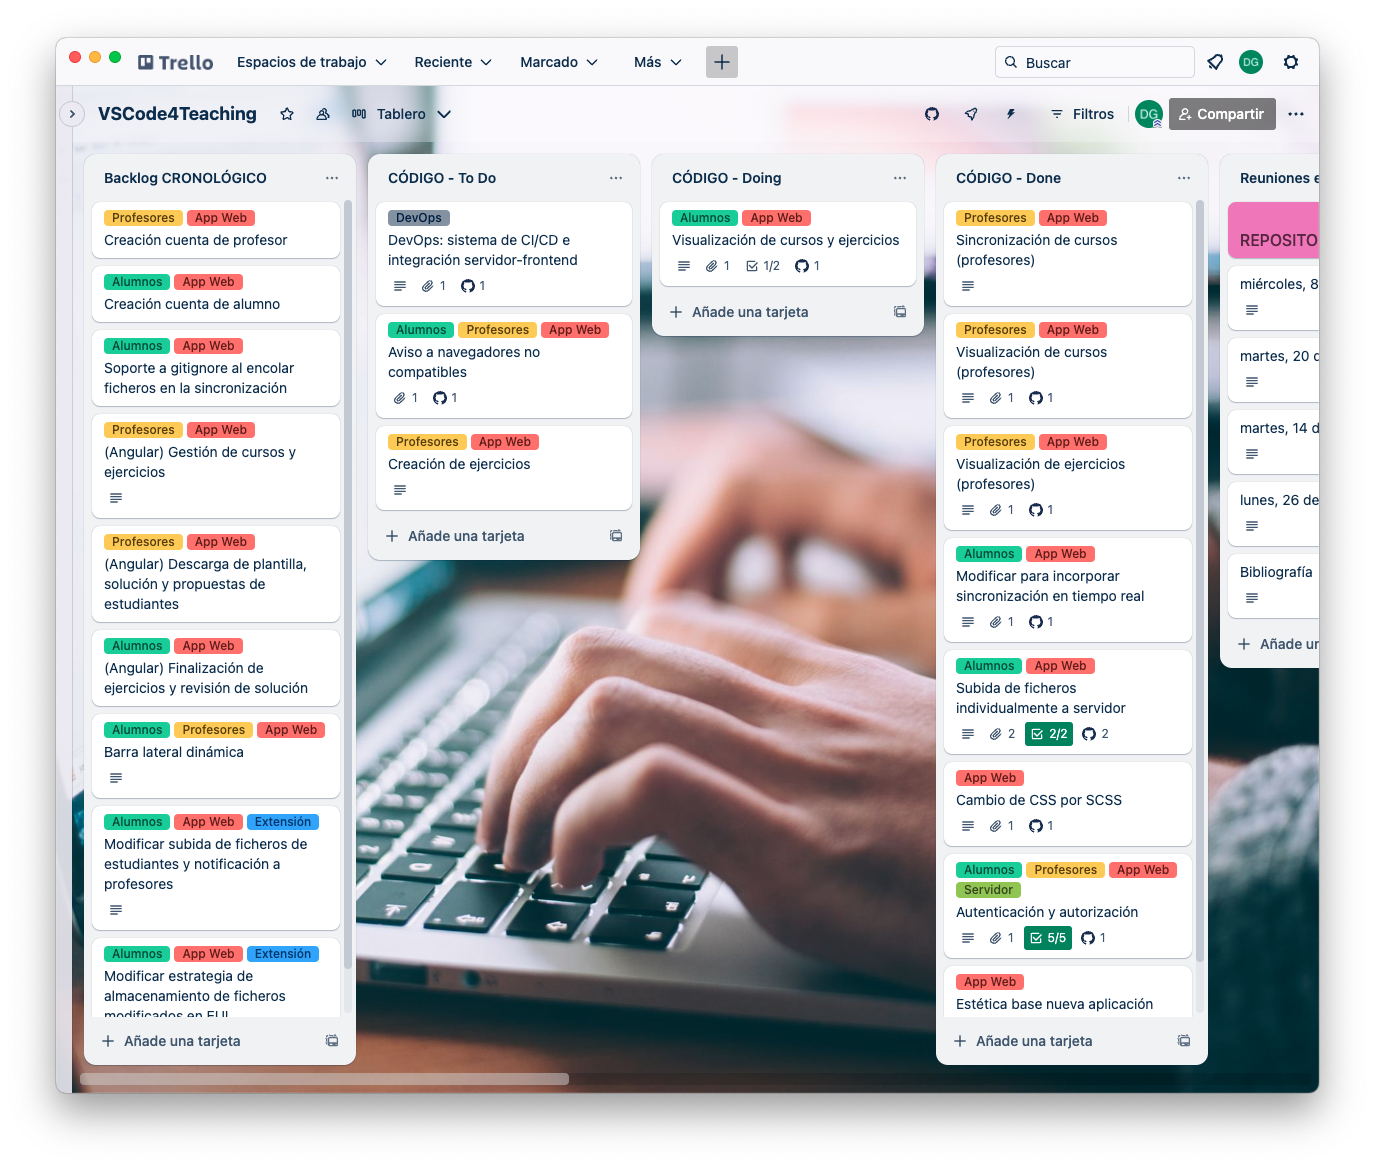
\includegraphics[width=\textwidth]{imagenes/utilizadas/3-2-herramientas/trello.png}
    \caption{Vista del tablero Trello empleado para la gestión del proceso \textit{software}.}
    \label{fig:tableroTrello}
\end{figure}
\section{Metodología: proceso \textit{software}}
\label{sec:metodologia}

La historia de la ingeniería del \textit{software}, aunque corta en el tiempo ---ya que surgió hace poco más de medio siglo---, es muy prolífica, y ha dado lugar a una gran lista de técnicas, herramientas y métodos organizativos empleados por los equipos para la correcta organización de los proyectos \textit{software}, favoreciendo la adecuada fragmentación de las tareas, su jerarquización y su planificación temporal para alcanzar un funcionamiento óptimo.

En el año 1986, Barry Boehm publicó un artículo en el que sentó las bases del \textbf{modelo en espiral} \cite{ModeloEspiral}, que, de forma resumida, propone que el proceso \textit{software} debe ser iterativo e incremental. Iterativo porque deben ejecutarse las mismas fases tantas veces como sea necesario (y no solo una, como proponía el método en cascada), e incremental porque cada iteración produce un nuevo aumento del \textit{software} construido.

Aunque sienta sus bases en trabajos anteriores, en 1995, Grady Booch propuso el enfoque realizado en Rational (perteneciente posteriormente a IBM) de un proceso \textit{software} basado en componentes, dirigido por casos de uso, centrado en la arquitectura y con un carácter iterativo e incremental. El posteriormente denominado \textbf{proceso unificado de desarrollo} tras la publicación realizada en 1999 por Booch, Jacobson y Rumbaugh \cite{RUP}, conocido por sus siglas RUP (del inglés \textit{Rational Unified Process}), es un proceso que pone en el centro de su ejecución los casos de uso, que sirven como enlace entre los requisitos y el diseño e implementación; y la arquitectura, que es primordial para la posterior construcción y evolución del sistema desarrollado. Hace un uso intensivo del lenguaje unificado de modelado (UML, por sus siglas en inglés \textit{Unified Model Language}) que, surgido en la misma corporación y divulgado por los mismos autores, establece una sintaxis gráfica para la expresión del funcionamiento y organización del \textit{software} ampliamente consolidada en esta ingeniería \cite{UML}.

También en 1999, Kent Beck publicó un libro acerca de un nuevo proceso \textit{software}: \textbf{eXtreme Programming} (XP) \cite{XP}. Propone una modificación del enfoque, haciendo mayor énfasis en la adaptabilidad frente al cambio que en la previsibilidad, considerando que los cambios sobre los requisitos son parte intrínseca de la naturaleza de los proyectos. En consonancia con este principio, XP propone nuevas técnicas para la ingeniería del \textit{software}, como la programación por pares (\textit{pair programming}), las buenas prácticas para la refactorización del código, el desarrollo guiado por las pruebas (TDD) o las historias de usuario, cuyo propósito es centrar cada requisito en el valor que aportará al usuario final.

Si bien los tres procesos desarrollados anteriormente sientan las bases de la ingeniería del \textit{software} tal como es en la actualidad, en la que la iteratividad e incrementalidad son los dos principios básicos que rigen todos los procesos \textit{software}, estos fueron opacados por la publicación del \textit{Manifiesto Ágil} en 2001 \cite{AgileManifesto}, que afirma que los procesos \textit{software} deben sentar sus bases en cuatro pilares: la preponderancia de individuos e interacciones sobre procesos y herramientas, el \textit{software} funcional sobre la documentación extensiva, la colaboración con el cliente sobre la negociación contractual y la respuesta frente al cambio sobre la planificación exhaustiva. Dentro de estos principios encajan múltiples procesos de anterior publicación, como Scrum (1995), Kanban (década de 1940) o XP, cuyas buenas prácticas gozan de una gran popularidad en la actualidad.

En general, y en esta ingeniería en particular, la historia es una gran fuente de aprendizaje. La ingeniería del \textit{software} ha aportado durante su aún breve historia una ingente cantidad de técnicas para facilitar la ejecución del proceso \textit{software} en todas sus etapas: la ingeniería de requisitos, el diseño y análisis, la implementación, la validación del \textit{software} y la entrega y el despliegue.

La mayoría de los procesos \textit{software} están ideados para su utilización en equipos de desarrollo, por lo que su aplicación directa en proyectos con características tan específicas como los Trabajos Fin de Grado resulta ineficaz. Sin embargo, son muchas las buenas prácticas que se pueden tomar del histórico de conjuntos de técnicas y herramientas como ayuda y soporte para generar un nuevo proceso \textit{ad hoc} para el contexto concreto del presente Trabajo.

Tal como propone el modelo en espiral desde hace cuarenta años, el proceso \textit{software} de este Trabajo Fin de Grado se ha realizado de forma iterativa e incremental, buscando la completitud de cada uno de los requisitos antes de seguir avanzando: en lugar de extraerlos para diseñarlos e implementarlos todos, se han extraído, diseñado e implementado cada uno por separado, dando lugar a la ejecución reitrada de pequeñas iteraciones completas conducentes hacia pequeños incrementos hasta alcanzar la evolución deseada.

Por tanto, aunque durante la ejecución de este nuevo hito evolutivo de \textit{VSCode4Teaching} no se ha seguido a rajatabla ningún proceso \textit{software} consolidado, son numerosas las prácticas empleadas que se han extraído de los procesos más extendidos. Así, el proceso es iterativo e incremental, tal como propone el modelo en espiral, alcanzando un total de trece iteraciones; cuida la arquitectura y la sitúa en el centro, como propone RUP, haciendo uso de UML como lenguaje de modelado; y emplea el formato de historias de usuario para la especificación de los requisitos funcionales, inspirándose en XP.

Tal como queda reflejado en la \referenciaSeccion{sec:herTrello}, que trata acerca de la herramienta para la planificación, durante este Trabajo se hace uso de un tablero inspirado en Kanban para la organización visual de las tareas, separándolas en tres columnas según su estado temporal: pendientes de hacer, en proceso y finalizadas. También inspirado en Kanban, se establece un límite al trabajo en progreso (WIP, del inglés \textit{Work In Progress}), de modo que no se realiza más de un requisito en paralelo. El tablero empleado toma de Scrum la idea de añadir una columna adicional para albergar una pila de puntos restantes para completar los requisitos conocidos del producto, el \textit{product backlog}, del que se van extrayendo tarjetas que, en este caso, representan historias de usuario (XP) que quedan fraccionadas e introducidas en otra pila específica para la actual iteración, coincidente en este caso con la columna de tareas pendientes de iniciar.


% Sección 4: Descripción informática

% Descripción del proyecto realizado.
% Después de unos párrafos introductorios el capítulo se divide en subcapítulos.
% Extensión recomendada: de 25 a 35 páginas.
% \afterpage{\blankpage}
\chapter{Descripción informática}
\label{cap:descInformatica}

Se recoge en esta sección la información detallada acerca del desarrollo ejecutado para la materialización en el proyecto \textit{VSCode4Teaching} de los objetivos propuestos en el \referenciaCapitulo{cap:objetivos}. Se introduce siguiendo el orden propio de los procesos \textit{software}: la \referenciaSeccion{sec:requisitos} introduce la enumeración de los requisitos derivados de los objetivos, la \referenciaSeccion{sec:diseñoArquitectura} versa sobre el diseño y arquitectura del proyecto y las modificaciones realizadas a este respecto, la \referenciaSeccion{sec:implementacion} desarrolla pormenorizadamente la consecución de cada requisito establecido, la \referenciaSeccion{sec:verificacion} detalla los mecanismos para la garantía de la calidad del \textit{software} y la \referenciaSeccion{sec:distribucion} abarca la distribución del código fuente y de los artefactos del proyecto.

% Sección 4.1: Requisitos.
% Descripción detallada de las funcionalidades que tendría que implementar la aplicación (pues se asume que los
% requisitos se escriben antes de empezar el desarrollo). Pueden tener forma de historias de usuario o bien ser una
% lista de requisitos funcionales y no funcionales.
\section{Extracción de requisitos}
\label{sec:requisitos}
Tomando como base el objetivo principal del proyecto (véase el \referenciaCapitulo{cap:objetivos}), y los distintos objetivos articulados en torno a él, el primer paso para acometer la descripción informática del trabajo es la enumeración de sus requisitos, reflejando breve, clara y concisamente las tareas que se ejecutarán.

Este Trabajo Fin de Grado recoge dos tipos de requisitos: funcionales y no funcionales. Se asocia a cada requisito un identificador de la forma \texttt{RX-Y}, donde \texttt{X} designa el tipo de requisito (\texttt{F} para funcionales y \texttt{N} para no funcionales) e \texttt{Y} es un valor numérico correlativo. El uso de estos identificadores quedará extendido a todo el presente documento.

\subsection{Requisitos funcionales}
\label{subsec:listaReqsFuncionales}
Se introducen a continuación los requisitos funcionales, que son aquellos que tienen como fin proporcionar mecanismos que permitan a los usuarios realizar procesos de negocio que les aporten valor; esto es, los conducentes a la incorporación de nueva funcionalidad en la aplicación.

Se recogen utilizando el formato típico de las ``historias de usuario'', una práctica extraída de eXtreme Programming (XP) \cite{XP_HistoriasUsuario}, redactándolos en un formato común preestablecido que es claro, conciso y fácilmente comprensible que sitúa en un papel preponderante las necesidades de los usuarios finales. Los requisitos son:
\begin{itemize}
    \item \texttt{\textbf{RF-1}}: como usuario registrado en \textit{VSCode4Teaching}, quiero poder acceder a mis cursos y ejercicios. Para ello, quiero poder iniciar sesión con mis credenciales para autenticarme y obtener acceso a mi información (\texttt{\textbf{RF-1.1}}) y, además, quiero poder visualizar mis cursos impartidos o matriculados y mis ejercicios (\texttt{\textbf{RF-1.2}}).
    \item \texttt{\textbf{RF-2}}: como profesor, quiero poder crear ejercicios nuevos en los cursos que imparto proporcionando una plantilla inicial y, opcionalmente, una propuesta de solución para que los alumnos puedan resolverlos.
    \item \texttt{\textbf{RF-3}}: como profesor, quiero poder visualizar en tiempo real información básica sobre el progreso de los estudiantes al realizar los ejercicios que he propuesto para poder conocer en todo momento la situación en que se encuentra cada ejercicio y cada estudiante.
    \item \texttt{\textbf{RF-4}}: como profesor, quiero poder descargar cuando lo desee los ficheros que compongan las propuestas de resolución de los ejercicios de los estudiantes para poder almacenarlas y visualizarlas, así como conocer de qué estudiante es cada una de ellas para poder asociar las distintas entregas con sus autores.
    \item \texttt{\textbf{RF-5}}: como profesor, quiero poder configurar los parámetros que determinan si la solución de los ejercicios es pública y si los estudiantes pueden editar sus propuestas tras descargarla para poder tener el control completo sobre cuándo se divulga la solución propuesta.
    \item \texttt{\textbf{RF-6}}: como profesor, quiero poder gestionar qué usuarios forman parte de mi curso para poder matricular o revocar el acceso de los estudiantes y para poder incorporar o eliminar a otros profesores.
    \item \texttt{\textbf{RF-7}}: como profesor, quiero tener la capacidad de compartir un código único de cada uno de mis cursos para poder dárselo a los estudiantes y que, de ese modo, se automatriculen en mi curso.
    \item \texttt{\textbf{RF-8}}: como alumno, quiero poder inscribirme en un cursos nuevos utilizando códigos proporcionados por los profesores para poder realizar sus ejercicios.
    \item \texttt{\textbf{RF-9}}: como alumno, quiero poder seleccionar un directorio de mi ordenador y usarlo para poder visualizar los ejercicios de un curso y sus ficheros.
    \item \texttt{\textbf{RF-10}}: como alumno, quiero poder iniciar un ejercicio nuevo y descargar su plantilla o reanudar un ejercicio y descargar mi progreso para poder realizarlo.
    \item \texttt{\textbf{RF-11}}: como alumno, quiero poder sincronizar automáticamente los ejercicios cuando los modifico y revisar el progreso de la sincronización para asegurarme de que se está almacenando correctamente.
    \item \texttt{\textbf{RF-12}}: como alumno, quiero poder marcar un ejercicio como finalizado para indicárselo al profesor y, de ese modo, consolidar el estado final de mi propuesta, ya que no podré volver a editarla.
\end{itemize}

\subsection{Requisitos no funcionales}
\label{subsec:listaReqsNoFuncionales}
Se recogen a continuación los requisitos no funcionales, que son aquellos que tienen como fin la mejora de los atributos de calidad del proyecto y de su \textit{software}, atendiendo a necesidades existentes alrededor de la funcionalidad que aportan valor al \textit{software} en sí mismo y, en consecuencia, a los usuarios. Estos son:
\begin{itemize}
    \item \texttt{\textbf{RN-1}}: mostrar un aviso en los navegadores no compatibles con la \textit{File System Access API}.
    \item \texttt{\textbf{RN-2}}: generar un aspecto visual común para la aplicación web de \textit{VSCode4Teaching} que sea intuitivo, fácil de comprender y coherente con la extensión para Visual Studio Code preexistente.
    \item \texttt{\textbf{RN-3}}: mejorar el sistema de autenticación existente para encriptar el \textit{token} JWT\footnote{JWT. Véase la \referenciaSeccion{subsec:rn3}.} mediante cifrado simétrico.
    \item \texttt{\textbf{RN-4}}: adaptar la generación de imágenes Docker del servidor para incorporar la aplicación web.
    \item \texttt{\textbf{RN-5}}: migrar el sistema de integración continua de Travis CI a GitHub Actions, adaptarlo a la nueva composición del proyecto y ampliar su alcance y tareas realizadas.
\end{itemize}


% Sección 4.2: Arquitectura y Análisis.
% Descripción de los aspectos de alto nivel de la aplicación.
% Diagramas de clases de análisis, diagramas de clases de diseño, etc.
% Se debe incluir la suficiente información para que el lector pueda entender la estructura de alto nivel del
% software desarrollado. Se pueden incluir diagramas de casos de uso si se considera útil.
\input{secciones/4-descripcionInformatica/4-2-diseñoArquitectura.tex}

% Sección 4.3: Diseño e implementación.
% Descripción de algún aspecto relevante de la implementación que quiera mencionarse.
% Por ejemplo se podría incluir alguno de los siguientes aspectos: algoritmo complejo que se haya tenido que
% desarrollar, integración entre librerías problemática, resolución de algún bug que haya sido especialmente
% problemático o ocalizar en alguna parte del desarrollo y describirla en más detalle.
% En esta sección se pueden incluir fragmentos de código fuente.
% En este apartado se pueden incluir algunas métricas del proyecto (No de clases, líneas de código, etc...).
% También se puede incluir la evolución del repositorio de github (gráfico de commits por día).
\section{Implementación}
\label{sec:implementacion}
Tras el establecimiento de los requisitos abarcados durante este hito evolutivo de \textit{VSCode4Teaching} en la \referenciaSeccion{sec:requisitos} y desarrollados tanto el diseño de cada componente como la arquitectura del proyecto en la \referenciaSeccion{sec:diseñoArquitectura}, se describe a continuación el proceso de implementación de los requisitos, desarollando para cada uno la necesidad que busca resolver y el valor que aporta al usuario o al proyecto \textit{software}.

\subsection{Requisitos funcionales}
\label{subsec:reqsFuncionales}
\subsubsection{\texttt{RF-1}: autenticación de usuarios y visualización de sus recursos asociados}
\label{subsec:rf1}

Este requisito establece la necesidad de que los usuarios de \textit{VSCode4Teaching} puedan autenticarse en la aplicación web para visualizar únicamente sus recursos legítimamente accesibles. Cabe dividir este requisito en dos partes: la autenticación (\texttt{RF-1.1}) y la visualización de los cursos asociados (\texttt{RF-1.2}).

El requisito \texttt{RF-1.1} establece la necesidad de que los usuarios puedan iniciar sesión para autenticarse utilizando su nombre de usuario y contraseña asociada, garantizando así que son quien dicen ser. Para ello, la aplicación web introduce un formulario que permite a los usuarios introducir las credenciales que ya venían utilizando para la verificación de su identidad en la extensión para Visual Studio Code en versiones anteriores, tal como refleja la \referenciaFigura{fig:reqf1-1}.

\begin{figure}[ht]
    \centering
    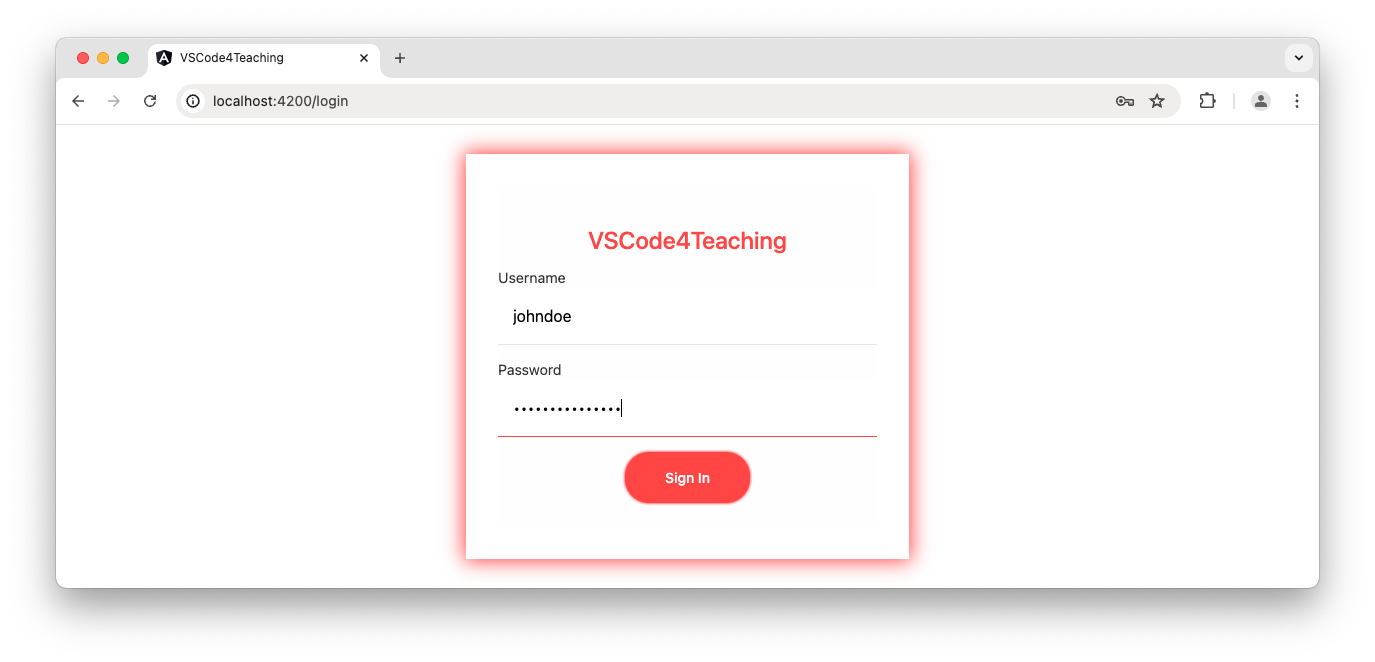
\includegraphics[width=\textwidth]{imagenes/utilizadas/4-3-implementacion/rf1-1.png}
    \caption{Formulario de inicio de sesión para usuarios registrados en la aplicación web.}
    \label{fig:reqf1-1}
\end{figure}

Una vez cumplimentado, las credenciales se envían al servidor y, en caso de ratificarse su validez, se genera un \textit{token} relativo a la sesión activa del usuario que queda almacenado en el contexto de la pestaña activa mediante el uso del \textit{sessionStorage}, que es un almacenamiento del navegador que permite almacenar pares clave-valor que persisten únicamente al contexto de la página que los crea (por contraposición con el \textit{localStorage}, que persiste a la finalización de la sesión activa salvo que se cierre la sesión ex profeso).

Por otro lado, el requisito \texttt{RF-1.2} especifica que los usuarios autenticados deben poder visualizar los recursos que tenga asociados a su cuenta. Para ello, una vez que los usuarios inician sesión en la aplicación, visualizan una pantalla de inicio que muestra los cursos de los que forman parte (\referenciaFigura{fig:reqf1-2}) que varía según el rol: mientras que los estudiantes tienen un botón para acceder a la pantalla en la que comienzan a realizar ejercicios (\referenciaConTT{subsec:rf9}{RF-9}), los docentes acceden a una interfaz (\referenciaFigura{fig:reqf1-3}) en la que pueden visualizar los ejercicios de los que dispone el curso con información básica sobre el progreso de cada uno y, además, crear nuevos ejercicios (\referenciaConTT{subsec:rf2}{RF-2}), gestionar los alumnos matriculados (\referenciaConTT{subsec:rf6}{RF-6}) y compartir el curso (\referenciaConTT{subsec:rf7}{RF-7}).

\begin{figure}[ht]
    \centering
    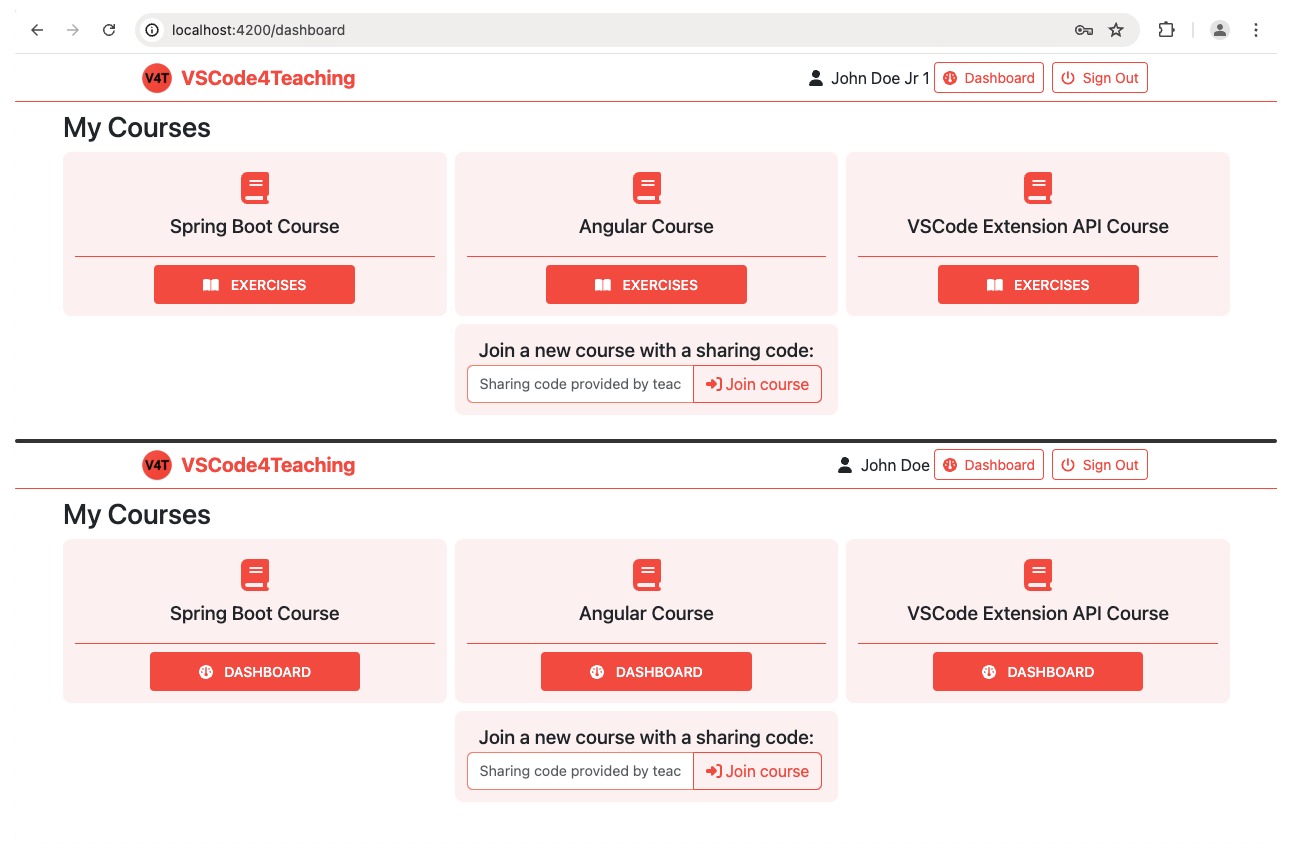
\includegraphics[width=\textwidth]{imagenes/utilizadas/4-3-implementacion/rf1-2.png}
    \caption{Pantalla de inicio para usuarios autenticados, tanto estudiantes (arriba) como docentes (abajo).}
    \label{fig:reqf1-2}
\end{figure}

\begin{figure}[ht]
    \centering
    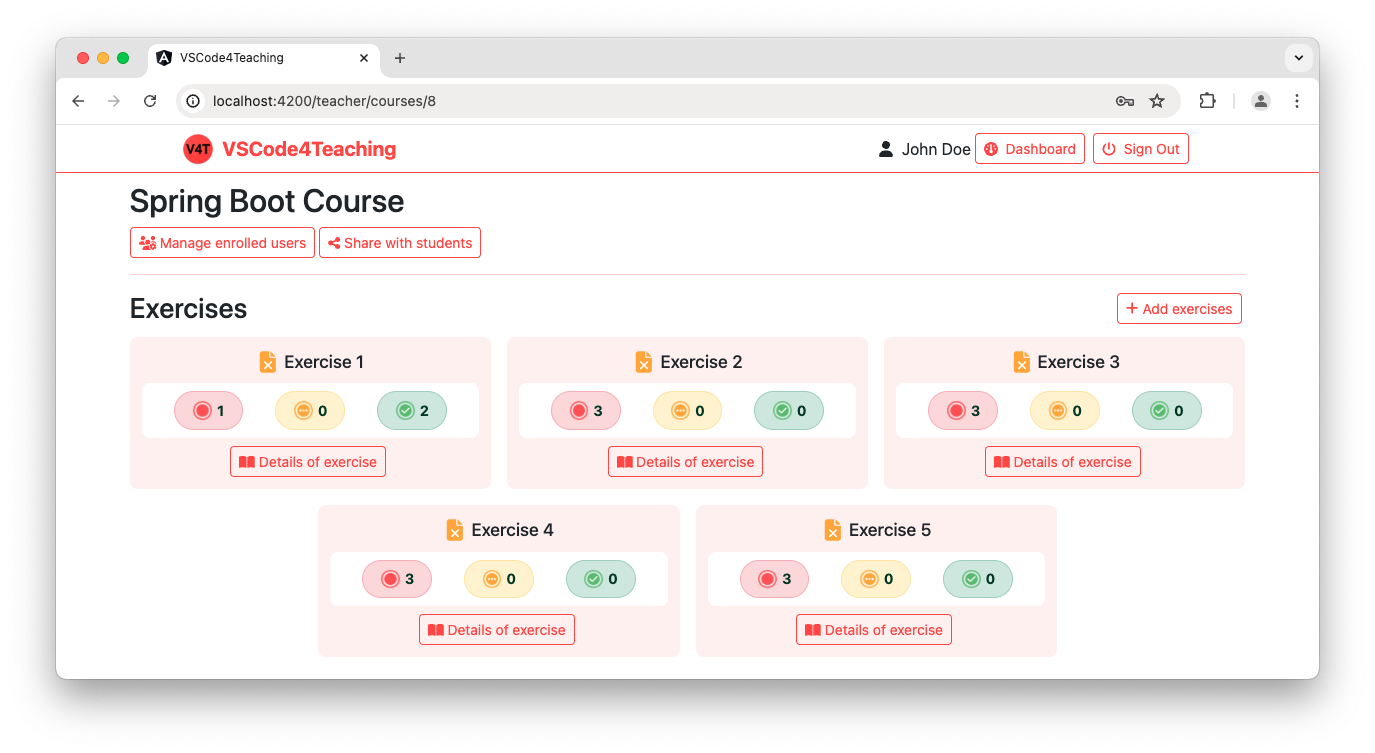
\includegraphics[width=\textwidth]{imagenes/utilizadas/4-3-implementacion/rf1-3.png}
    \caption{Interfaz principal para docentes acerca de cada uno de sus cursos impartidos.}
    \label{fig:reqf1-3}
\end{figure}

\subsubsection{\texttt{RF-2}: creación de nuevos ejercicios}
\label{subsec:rf2}

Los docentes tienen la capacidad de añadir ejercicios nuevos en los cursos que imparten. En la extensión, disponen de sendos botones para añadir un solo ejercicio o varios contenidos en un mismo directorio. Para replicar este comportamiento en la aplicación web, en la pantalla que les permite visualizar el detalle de sus cursos (introducida en el \referenciaConTT{subsec:rf1}{RF-1.2}) disponen de un botón ``Add exercises'' (añadir ejercicios) que despliega un modal con todos los elementos y controles necesarios para poder crear nuevos ejercicios.

En un primer momento, el modal solicita al profesor que seleccione un directorio disponible en su sistema local de ficheros. Una vez elegido el directorio, el navegador solicitará permiso de lectura de sus contenidos a través de la \textit{File System Access API} (véase la \referenciaSeccion{subsec:tecFSA}) y, una vez concedido, se determinará automáticamente si el directorio contiene únicamente la plantilla o si tiene, además, propuesta de solución del docente. Se considera que un ejercicio dispone de plantilla de solución si su directorio raíz contiene, al menos, dos directorios \textit{template} y \textit{solution} cuyos contenidos serán tomados, respectivamente, como la plantilla y la propuesta de solución ---formato ya empleado anteriormente en la extensión---; interpretándose en otro caso que todos los contenidos conforman la plantilla. Esta exploración puede realizarse directamente en el directorio elegido o en cada subdirectorio que contenga, considerando cada uno de ellos como un nuevo ejercicio y determinando en cada caso si tienen propuesta de solución o únicamente plantilla.

\begin{figure}[ht]
    \centering
    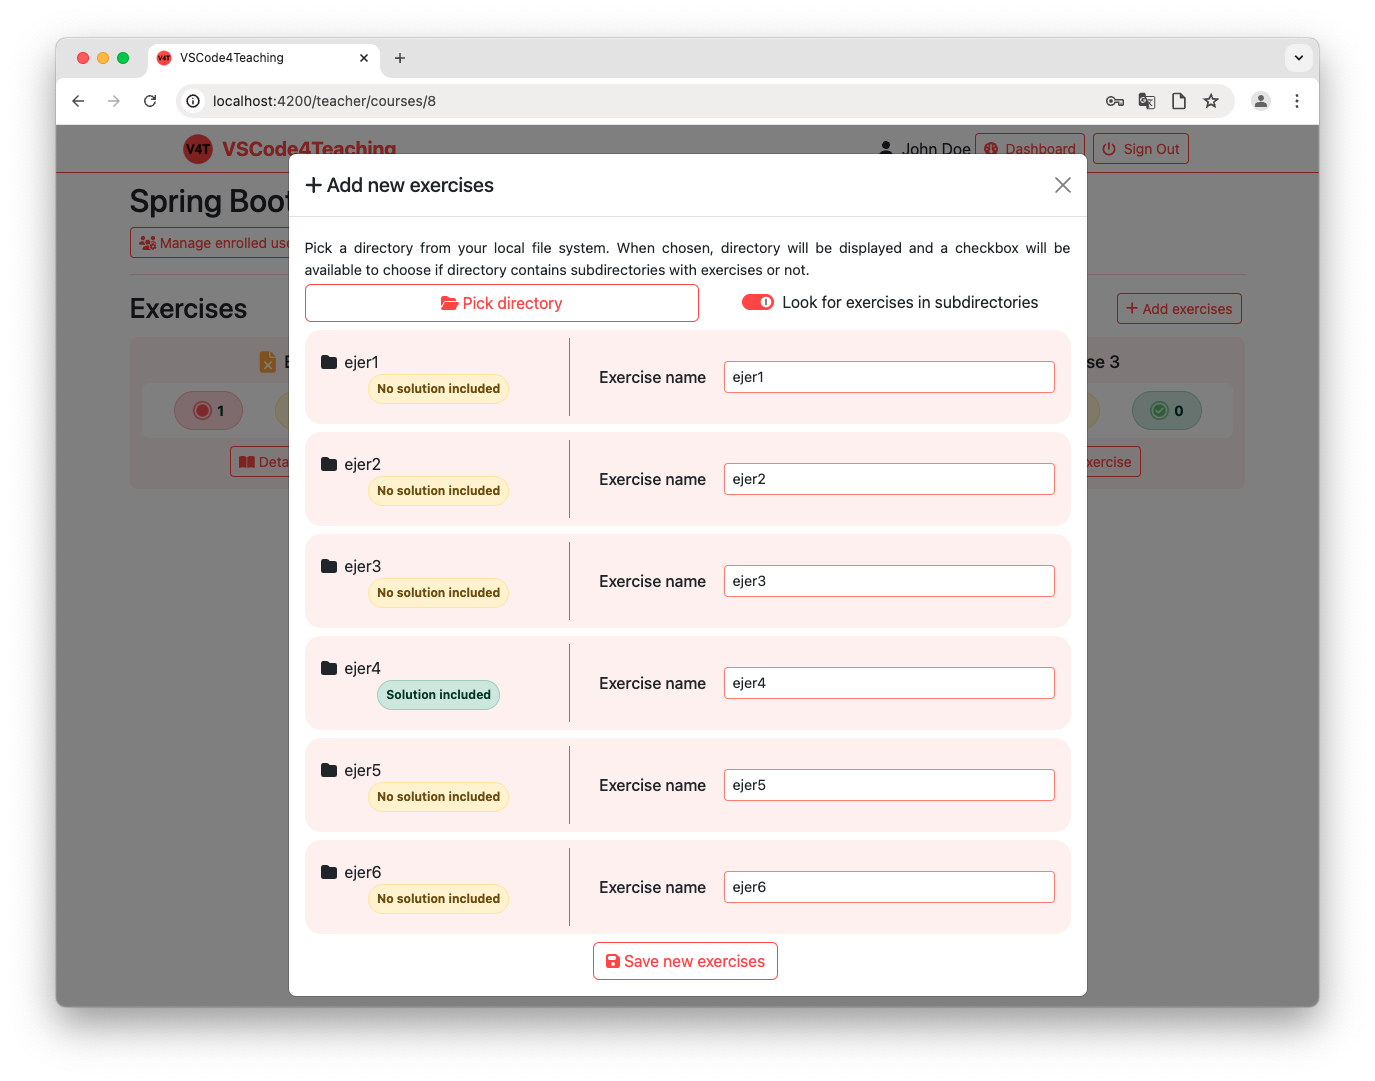
\includegraphics[width=\textwidth]{imagenes/utilizadas/4-3-implementacion/rf2-1.png}
    \caption{Ventana modal para la creación de nuevos ejercicios tras analizar los contenidos del directorio elegido.}
    \label{fig:reqf2-1}
\end{figure}

Una vez elegido un directorio y determinado si se desea emplear directamente esta carpeta o sus contenidas, se muestra una lista con los ejercicios reconocidos, mostrando para cada uno el directorio local del que proceden y un campo que permite configurar su nombre, tomando por defecto el nombre del directorio que contiene los ficheros asociados. Se muestra un ejemplo en la \referenciaFigura{fig:reqf2-1}, en la que se escoge revisar las carpetas contenidas en el directorio elegido, observando que únicamente una de ellas contiene una propuesta de resolución.

Cuando se han determinado los nombres para los ejercicios, es posible iniciar su creación. Este proceso, para cada ejercicio, ejecuta una primera petición para generar el ejercicio en el servidor y, cuando obtiene respuesta, se comprimen en el navegador los ficheros que conforman la plantilla, enviándola una vez comprimida en una nueva petición. En caso de incluir propuesta de solución, a este proceso se suma una nueva compresión y petición para guardar la propuesta de solución. Se ejecutan todos los procesos para la creación de ejercicios concurrentemente, tal como evidencia la \referenciaFigura{fig:reqf2-2}, informando a través de una barra de progreso e indicadores de estado del avance del proceso para cada ejercicio. Solo cuando hayan terminado todos los procesos, el modal podrá ser cerrado.

\begin{figure}[ht]
    \centering
    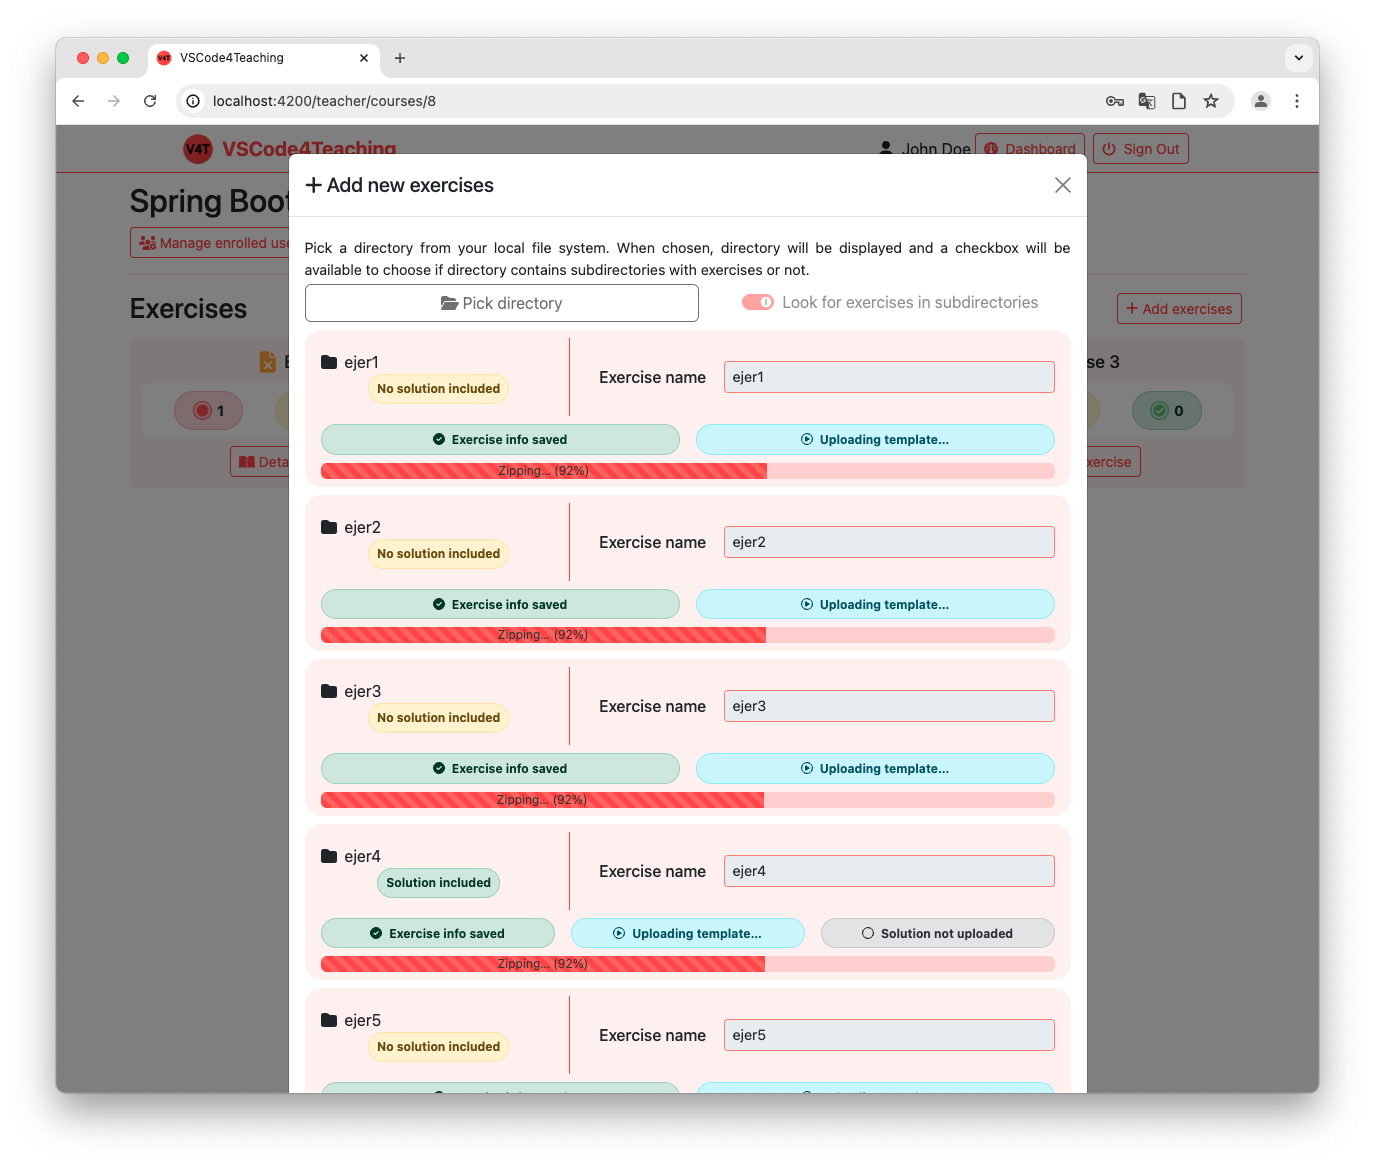
\includegraphics[width=\textwidth]{imagenes/utilizadas/4-3-implementacion/rf2-2.png}
    \caption{Instantánea de la ejecución del proceso de creación de nuevos ejercicios.}
    \label{fig:reqf2-2}
\end{figure}

\subsubsection{\texttt{RF-3}: seguimiento en tiempo real de progreso de ejercicios}
\label{subsec:rf3}

Cuando utilizan la extensión para Visual Studio Code, los docentes disponen de la capacidad para visualizar el \textit{dashboard} de un ejercicio, que muestra métricas actualizadas en tiempo real sobre el progreso de los estudiantes. Del mismo modo, la extensión incorpora una pantalla muy parecida que permite realizar un seguimiento en tiempo real sobre cada ejercicio de los cursos impartidos por un docente.

\begin{figure}[ht]
    \centering
    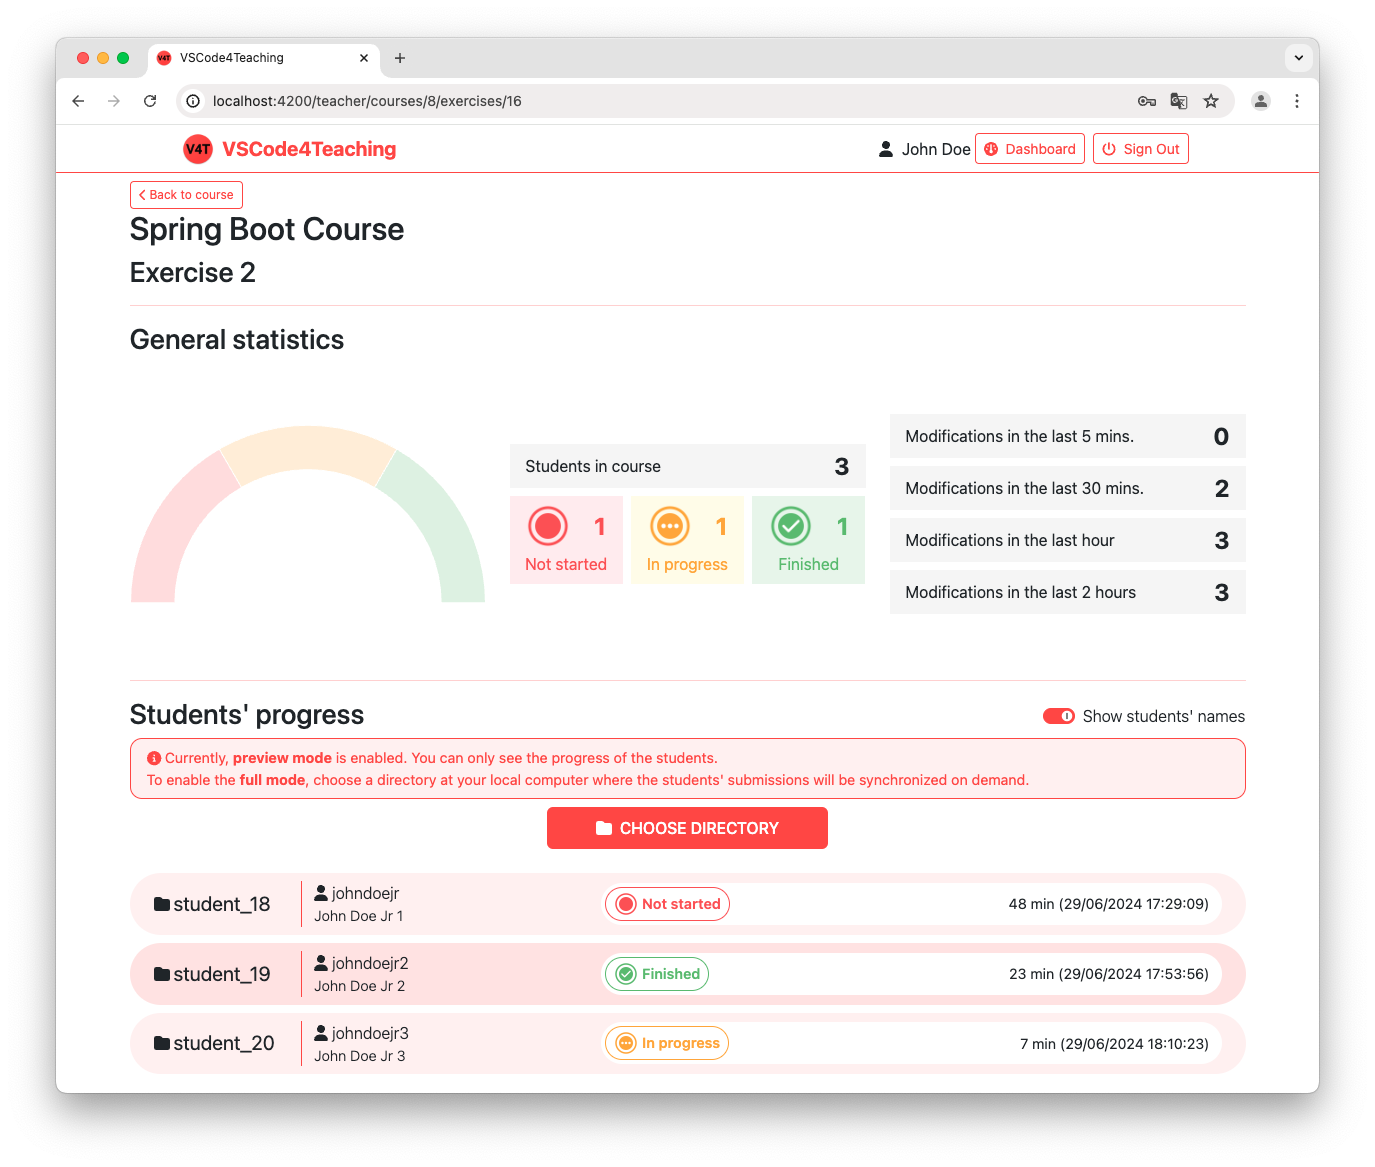
\includegraphics[width=\textwidth]{imagenes/utilizadas/4-3-implementacion/rf3-1.png}
    \caption{\textit{Dashboard} de un ejercicio en la aplicación web con métricas actualizadas en tiempo real para el seguimiento del progreso de los estudiantes.}
    \label{fig:reqf3-1}
\end{figure}

Se incluye una captura de esta visualización en la \referenciaFigura{fig:reqf3-1}. Esta visualización permite ver a los docentes rápidamente cuántos estudiantes hay matriculados en el curso ---y, por tanto, cuántos alumnos realizarán potencialmente el ejercicio---, desgranados debajo según el progreso, diferenciando los que no lo han iniciado, los que están realizándolo y los que lo han finalizado, incluyendo una gráfica semicircular representativa adyacente. Además, también se muestra cuántos estudiantes han modificado su propuesta en los últimos cinco y treinta minutos, en la última hora y dos horas. Debajo de estas estadísticas generales, es posible visualizar el progreso individualizado de cada estudiante, que se muestra de forma anónima: junto a cada directorio de cada propuesta de resolución aparecen el estado del ejercicio y la fecha y tiempo transcurrido tras la última modificación. Es posible asociar cada propuesta de resolución a su autor al modificar el control ``Show students' names'', lo que hará que se muestre en cada fila, además, el apodo y nombre completo de cada estudiante.

La extensión permite disponer del \textit{dashboard} en dos formatos: en forma de previsualización, mostrando únicamente las métricas anteriormente relatadas, o en formato completo, permitiendo abrir los ficheros que componen la propuesta de cada estudiante. Análogamente, la aplicación web permite visualizar únicamente las métricas en formato de previsualización y, además, da al docente la opción de escoger un directorio local para descargar en él bajo demanda las distintas propuestas de los estudiantes, tal como se detalla en el requisito \referenciaConTT{subsec:rf4}{RF-4}.

\subsubsection{\texttt{RF-4}: obtención bajo demanda de ficheros de ejercicios}
\label{subsec:rf4}

\begin{figure}[ht!]
    \centering
    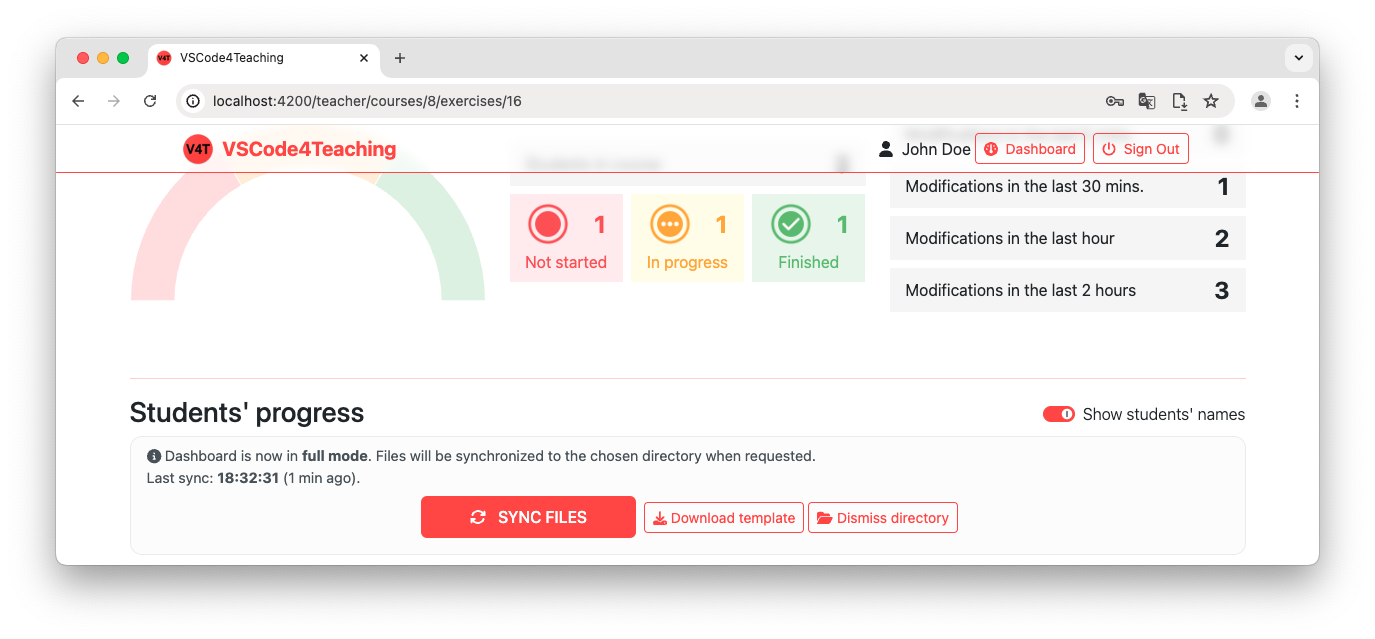
\includegraphics[width=\textwidth]{imagenes/utilizadas/4-3-implementacion/rf4-1.png}
    \caption{Fragmento del \textit{dashboard} que informa sobre la descarga de los ficheros de las propuestas de resolución de los estudiantes.}
    \label{fig:reqf4-1}
\end{figure}

El \textit{dashboard} de cada ejercicio disponible en la extensión permite, en su formato completo, abrir los ficheros que conforman la propuesta de resolución de cada estudiante y, además, visualizar gráficamente en Visual Studio Code las diferencias existentes entre las propuestas y la plantilla original. Análogamente, y dentro de las capacidades que permiten las tecnologías empleadas (descritas en la \referenciaSeccion{subsec:tecAppWeb}), la aplicación web brinda a los docentes la capacidad de descargar bajo demanda todas las propuestas de resolución para poder visualizarlas en local en el editor de su preferencia.

El requisito \referenciaConTT{subsec:rf3}{RF-3} introduce el funcionamiento y las capacidades de las que dispone el \textit{dashboard} de ejercicios implementado en la aplicación web. En la sección acerca del progreso de los estudiantes, tal como se puede apreciar en la \referenciaFigura{fig:reqf3-1}, se dispone un botón ``Choose directory'' (elegir directorio) que permite a los docentes escoger una carpeta en su máquina sobre la que concederán permisos de lectura y escritura para descargar en ella las propuestas de resolución de los estudiantes bajo demanda.

Tal como refleja la \referenciaFigura{fig:reqf4-1}, al escoger una carpeta local se habilitan nuevas opciones para los docentes, análogas al ``modo completo'' del \textit{dashboard} de la extensión, permitiendo la sincronización de los ficheros de los estudiantes bajo demanda, registrando cuándo fueron descargados por última vez. Esta sincronización es unidireccional, ya que no se registran las modificaciones locales realizadas por los docentes y, además, la descarga sobrescribe los ficheros previamente existentes en local. Se permite al profesor, adicionalmente, descargar la plantilla del ejercicio (y la propuesta de solución si la tuviera) en el mismo directorio.

\subsubsection{\texttt{RF-5}: configuración de publicación de solución de ejercicios}
\label{subsec:rf5}

\begin{figure}[!ht]
    \centering
    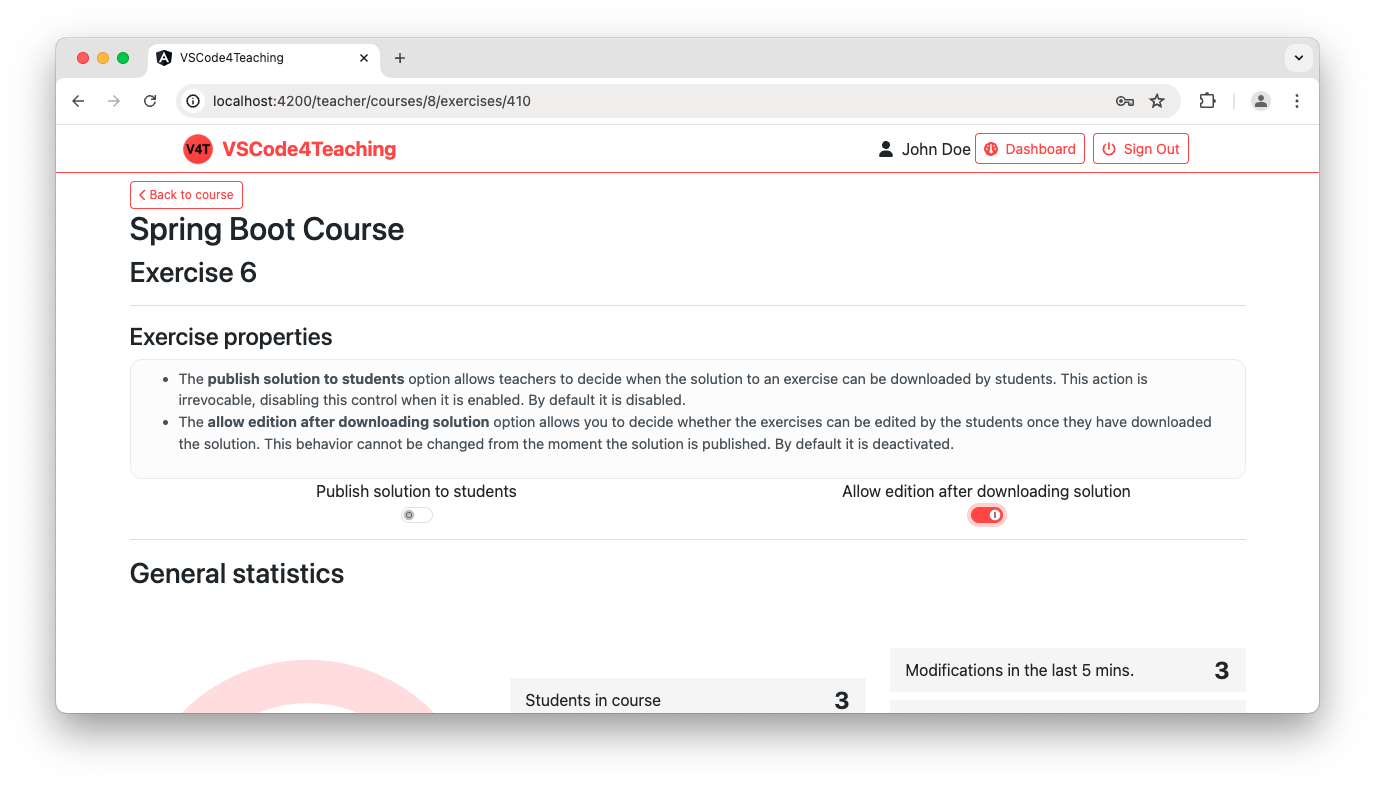
\includegraphics[width=0.9\textwidth]{imagenes/utilizadas/4-3-implementacion/rf5-1.png}
    \caption{Sección del \textit{dashboard} de los ejercicios que permite configurar los parámetros para la configuración de la disponibilidad y comportamiento de la descarga de la propuesta de solución del docente.}
    \label{fig:reqf5-1}
\end{figure}

Tal como se especifica en el requisito \referenciaConTT{subsec:rf2}{RF-2}, los ejercicios que los docentes añaden en sus cursos pueden tener asociada una propuesta de solución que los estudiantes pueden descargar en la extensión según dos parámetros de configuración de la disponibilidad de la solución que los docentes pueden ajustar en el \textit{dashboard} de cada ejercicio, tal como muestra la \referenciaFigura{fig:reqf5-1}. Los parámetros son:
\begin{itemize}
    \item \textit{Allow edition after downloading solution} (permitir edición tras descargar solución). Permite ajustar si los estudiantes pueden modificar sus propias propuestas tras descargar la solución o si, por el contrario, al descargar la propuesta de solución se deben impedir nuevas ediciones, marcándolo previamente como finalizado. Este parámetro se puede modificar mientras la solución no sea pública.
    \item \textit{Publish solution to students} (publicar solución a estudiantes). Permite configurar la disponibilidad para la descarga de la solución a los estudiantes, quienes dispondrán de un elemento gráfico en la extensión que les permitirá descargar la solución en local para, además, poder compararla mediante una interfaz gráfica para visualizar las diferencias existentes entre su propia propuesta y la solución del docente. La activación de la publicación impide la edición del parámetro anterior y, una vez publicada, esta configuración ya no puede revertirse.
\end{itemize}

\subsubsection{\texttt{RF-6}: gestión de matriculación de usuarios en cursos}
\label{subsec:rf6}

Cuando utilizan la extensión para Visual Studio Code, los docentes tienen la posibilidad de inscribir y eliminar estudiantes y otros profesores de sus cursos. Equivalentemente, se añade a la aplicación web la posibilidad de gestionar las matrículas de un curso. Para ello, tal como introduce el requisito \referenciaConTT{subsec:rf1}{RF-1.2}, los docentes disponen de un botón ``Manage enrolled users'' (gestionar usuarios inscritos) que despliega una ventana modal.

Este modal, tal como se muestra en la \referenciaFigura{fig:reqf6-1}, muestra una lista con todos los usuarios inscritos en el curso, diferenciando a los profesores de los estudiantes. A excepción del profesor creador, cada uno de estos usuarios puede ser eliminado del curso haciendo uso del botón dispuesto en cada fila. Adicionalmente, en la parte inferior se muestra un desplegable que contiene todos los usuarios potencialmente matriculables; esto es, a todos los usuarios salvo a aquellos que ya están matriculados. El profesor puede escoger uno de ellos y, mediante el botón adyacente, inscribirlo en el curso.

\begin{figure}[ht]
    \centering
    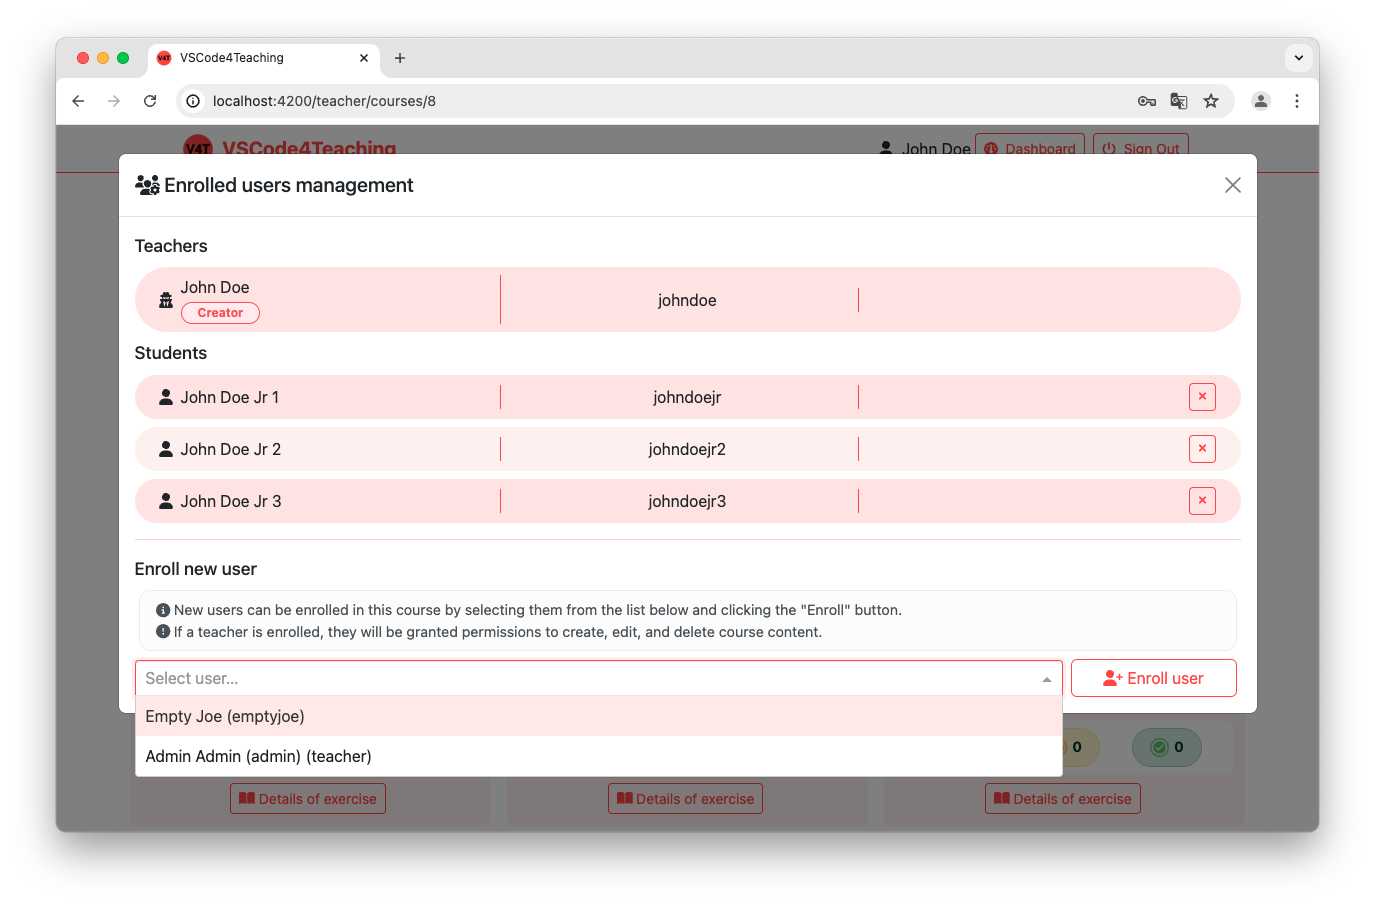
\includegraphics[width=\textwidth]{imagenes/utilizadas/4-3-implementacion/rf6-1.png}
    \caption{Visualización de la lista de usuarios inscritos a un curso y de las capacidades para añadir nuevos usuarios o revocar inscripciones.}
    \label{fig:reqf6-1}
\end{figure}

\subsubsection{\texttt{RF-7}: compartición de código asociado a un curso}
\label{subsec:rf7}

Existen dos formas para hacer que un estudiante quede matriculado en un curso, tanto en la extensión como en la aplicación web: puede ser inscrito manualmente por un profesor (\referenciaConTT{subsec:rf6}{RF-6}) o puede automatricularse (\referenciaConTT{subsec:rf8}{RF-8}), que requiere de un código que deben ser proporcionado por el docente.

La extensión permite a los docentes obtener un enlace al servidor de \textit{VSCode4Teaching} en uso que puede divulgar al estudiantado que desee que se automatricule. Este enlace incluye un código único que identifica biunívocamente cada curso existente en la plataforma. Para generarlo, la visualización de los cursos para docentes (\referenciaConTT{subsec:rf1}{RF-1.2}) dispone de un botón ``Share with students'' (compartir con estudiantes) que, tal como queda plasmado en la \referenciaFigura{fig:reqf7-1}, muestra a los docentes el código único para la automatrícula en el curso como, además, el enlace al servidor que los alumnos pueden abrir en el navegador para consultar información adaptada al caso del curso específicamente divulgado, incluyendo instrucciones acerca de cómo inscribirse en el curso compartido.

\begin{figure}[ht]
    \centering
    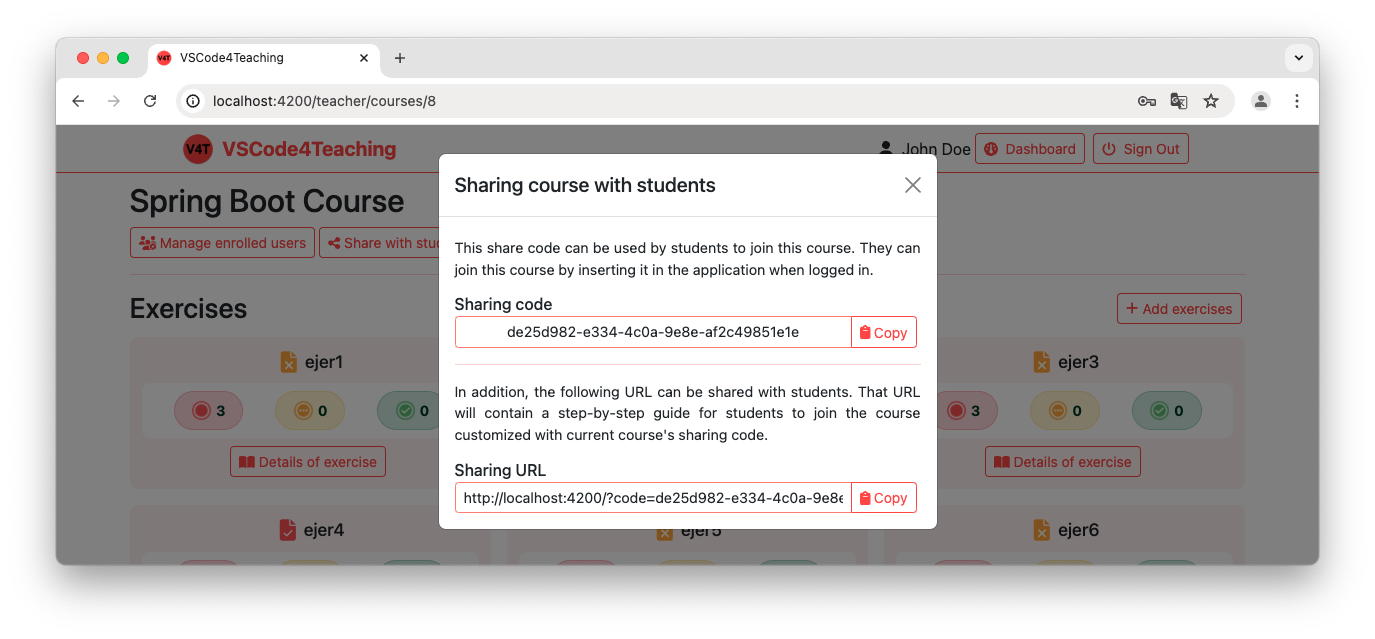
\includegraphics[width=\textwidth]{imagenes/utilizadas/4-3-implementacion/rf7-1.png}
    \caption{Información para la compartición del código único de automatrícula en un curso.}
    \label{fig:reqf7-1}
\end{figure}

\subsubsection{\texttt{RF-8}: automatriculación mediante código de compartición}
\label{subsec:rf8}

Los estudiantes pueden ser matriculados en los cursos manualmente por sus docentes (\referenciaConTT{subsec:rf6}{RF-6}) y, además, tienen la capacidad de inscribirse en cursos por sí mismos utilizando un código proporcionado por sus profesores, ya sea empleando la extensión para Visual Studio Code o a través de la aplicación web. Este requisito es complementario del \referenciaConTT{subsec:rf7}{RF-7}, por el que los docentes disponen de la capacidad para generar códigos de compartición para permitir la autoinscripción de estudiantes en sus cursos.

En caso de querer hacerlo a través de la aplicación web, los estudiantes deben iniciar sesión (\referenciaConTT{subsec:rf1}{RF-1.1}) y, dentro de su página principal, disponen de un campo de texto para introducir el código proporcionado por los docentes, tal como se aprecia en la \referenciaFigura{fig:reqf8-1} y, presionando el botón adyacente, pueden inscribirse en un nuevo curso.

\begin{figure}[ht]
    \centering
    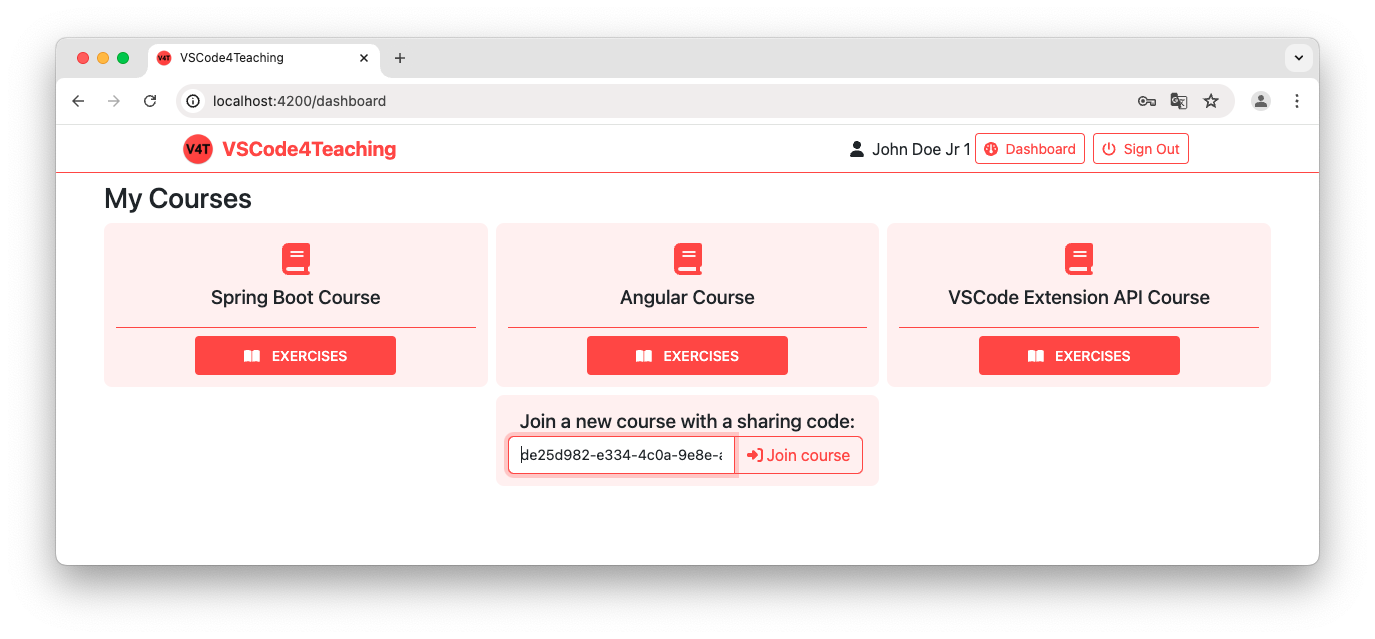
\includegraphics[width=\textwidth]{imagenes/utilizadas/4-3-implementacion/rf8-1.png}
    \caption{Página principal de los estudiantes en la aplicación web con un código de inscripción automática en un curso.}
    \label{fig:reqf8-1}
\end{figure}

\subsubsection{\texttt{RF-9}: visualización de un curso y sus ejercicios}
\label{subsec:rf9}

Una vez autenticados en \textit{VSCode4Teaching} (\referenciaConTT{subsec:rf1}{RF-1.1}), los estudiantes visualizan una pantalla principal o \textit{dashboard} en el que se muestran los cursos en los que están matriculados, tal como se desarrolla en el requisito \referenciaConTT{subsec:rf1}{RF-1.2}. En esta pantalla disponen de un botón ``Exercises'' (ejercicios) en cada curso que les permite acceder al detalle de los ejercicios de cada curso.

Cuando los estudiantes acceden a la visualización del detalle de un curso, la aplicación les solicita primeramente que escojan un directorio del sistema de ficheros de su computador local para alojar los contenidos de los ejercicios del curso, situación inicial que queda reflejada en la \referenciaFigura{fig:reqf9-1}. Si el estudiante ya realizó algún ejercicio, sea total o parcialmente, y mantuvo intacto el directorio que empleó ---esto es, respetando el formato de subdirectorios empleado en local por \textit{VSCode4Teaching}---, puede utilizar la misma carpeta para continuar trabajando, ya que coincidirá el estado de los ejercicios almacenados en local con el progreso sincronizado en el servidor y no se producirán desfases.

\begin{figure}[ht]
    \centering
    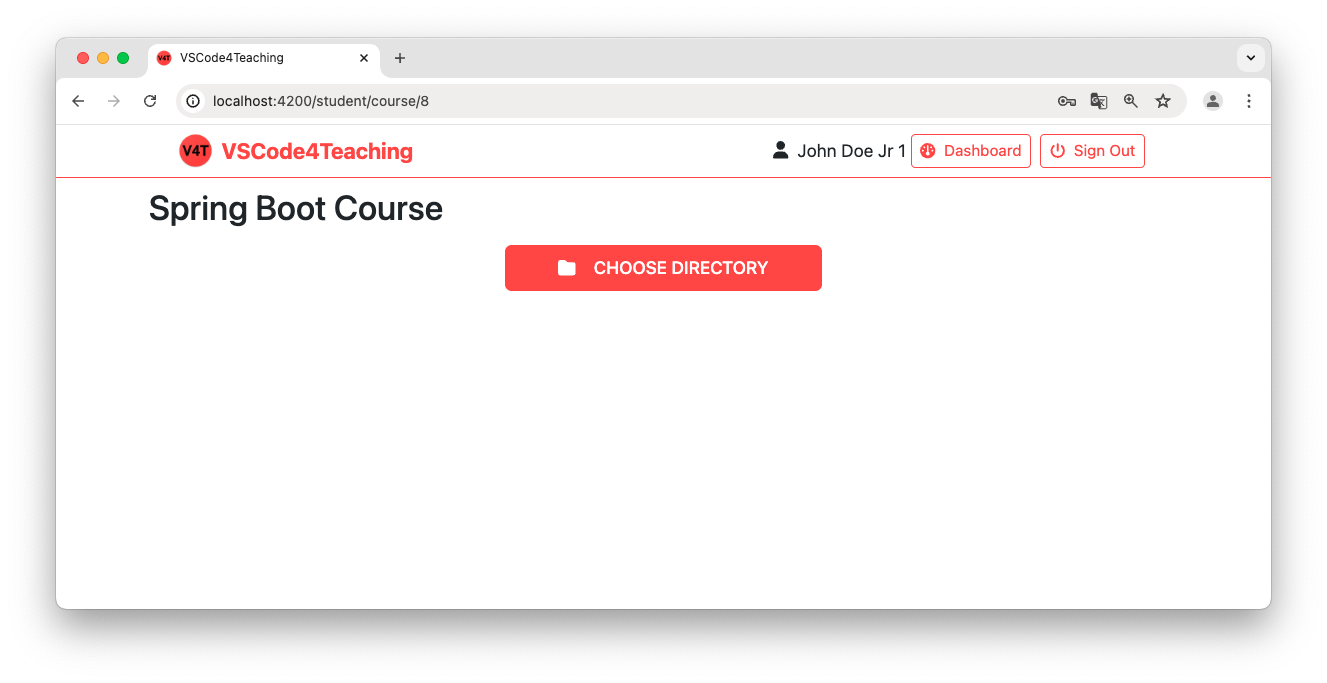
\includegraphics[width=\textwidth]{imagenes/utilizadas/4-3-implementacion/rf9-1.png}
    \caption{Situación inicial de los estudiantes al acceder al detalle de un curso y antes de elegir un directorio local.}
    \label{fig:reqf9-1}
\end{figure}

Una vez escogido el directorio, se muestra a los estudiantes el detalle de los ejercicios asociados al curso, sepárandolos en distintos paneles según su estado de ejecución: los ejercicios en progreso se sitúan en la parte superior, ubicando debajo los ejercicios no comenzados y los finalizados, tal como se refleja en la \referenciaFigura{fig:reqf9-2}. Esta ilustración permite apreciar que el estudiante tiene dos ejercicios pendientes de comenzar (``Exercise 2'' y ``Exercise 5''), ubicados dentro del panel sombreado en rojo con título ``Not started'' (no comenzado) y, además, ha finalizado un ejercicio (``Exercise 3'') que aparece dentro del panel sombreado en verde con título ``Finished'' (finalizado). A estos se suman dos ejercicios dentro del panel amarillo con título ``In progress'' (en progreso), que el estudiante podrá descargar o empezar a sincronizar, posibilidades implementadas en el requisito \referenciaConTT{subsec:rf10}{RF-10}.

\begin{figure}[ht]
    \centering
    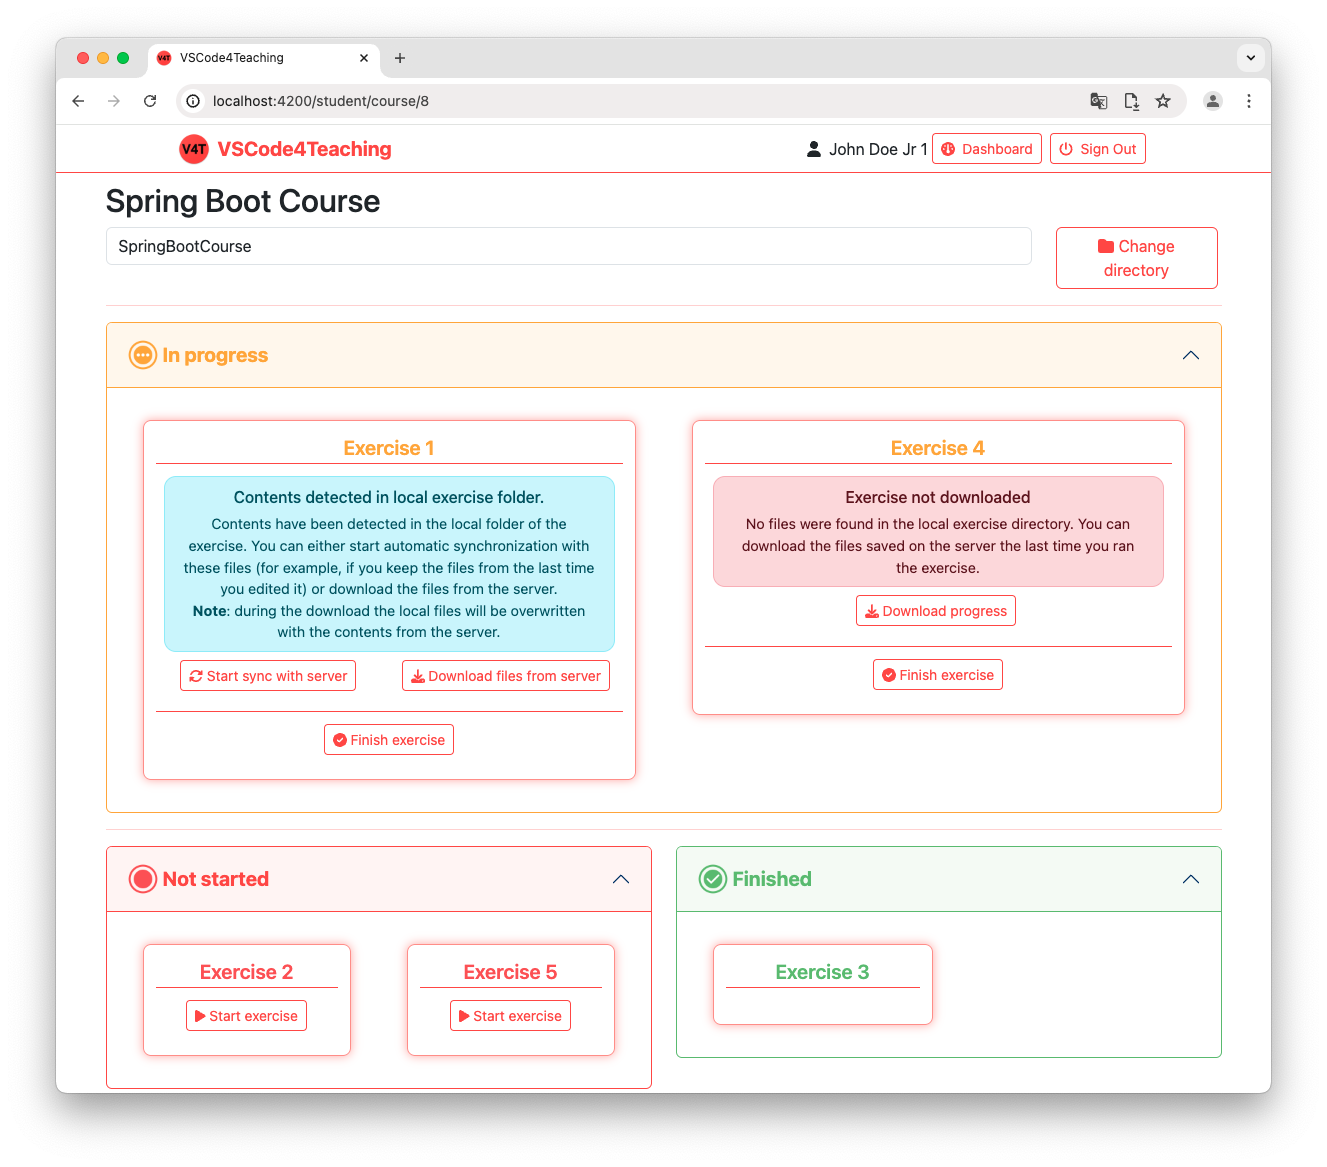
\includegraphics[width=\textwidth]{imagenes/utilizadas/4-3-implementacion/rf9-2.png}
    \caption{Visualización detallada de un curso matriculado por un estudiante con ejercicios ubicados en distintos paneles según su estado.}
    \label{fig:reqf9-2}
\end{figure}

\subsubsection{\texttt{RF-10}: descarga de los ficheros de una propuesta propia de resolución de un ejercicio}
\label{subsec:rf10}

Dentro de la visualización del detalle de un curso matriculado, y tras escoger un directorio local para sincronizar los ficheros, un estudiante puede visualizar todos los ejercicios del curso diferenciados en distintos paneles según su estado de ejecución, tal como especifica el \referenciaConTT{subsec:rf9}{RF-9}.

En el caso de los ejercicios en progreso, al escoger el directorio, la aplicación buscará si existe una versión local del ejercicio, transitando entre los distintos estados reflejados en la \referenciaFigura{fig:reqf10-1}. En caso de no existir ninguna carpeta hija del directorio elegido coincidente con un ejercicio en progreso, la aplicación informará al usuario de que deberá descargar el punto de progreso que haya almacenado en el servidor, tal como ocurre con el ``Exercise 4'' en la \referenciaFigura{fig:reqf9-2}. Si, por el contrario, existe un directorio local que coincida con el ejercicio en progreso, la aplicación pregunta al usuario si desea descargar la versión existente en remoto y sobrescribir los ficheros que colapsen respecto a la versión en local o si, por el contrario, desea iniciar de inmediato la sincronización con el servidor. Este primer escenario es el que sucede en el caso del ``Exercise 1'' de la \referenciaFigura{fig:reqf9-2}.

Estos dos estados iniciales están reflejados en la parte izquierda de la \referenciaFigura{fig:reqf10-1}. Al descargar el ejercicio, se transita al estado que se observa en la parte central de la representación, durante el que la aplicación descarga como fichero comprimido los contenidos del ejercicio proporcionados por el servidor y los descomprime en una carpeta propicia específica dentro del directorio elegido por el estudiante, informando de forma visual a través de dos indicadores del estado activo y una barra de progreso. Una vez preparado el directorio del ejercicio, sea porque ha finalizado la descarga y descompresión o porque se ha iniciado la sincronización de contenidos previamente existentes, se inicia la sincronización automática, reflejada visualmente como muestra la parte derecha de la \referenciaFigura{fig:reqf10-1}. Esta sincronización queda detalladamente explicada en el requisito \referenciaConTT{subsec:rf11}{RF-11}.

\begin{figure}[ht]
    \centering
    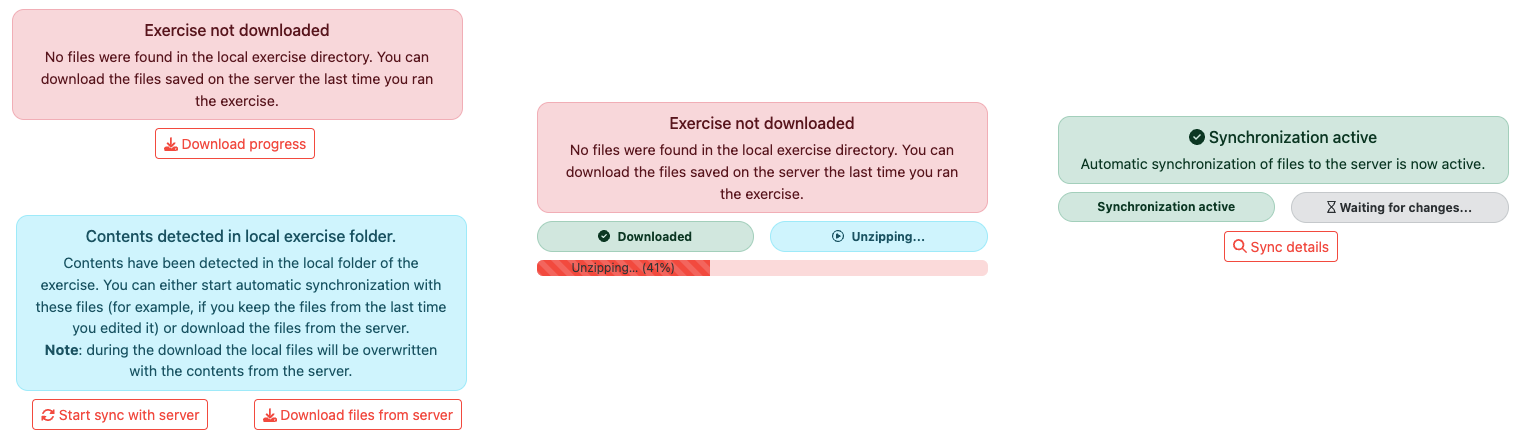
\includegraphics[width=\textwidth]{imagenes/utilizadas/4-3-implementacion/rf10-1.png}
    \caption{Representación de la evolución entre los posibles estados visuales de los ejercicios en progreso según su disponibilidad local.}
    \label{fig:reqf10-1}
\end{figure}

\subsubsection{\texttt{RF-11}: sincronización automática de las modificaciones en los ejercicios durante su realización}
\label{subsec:rf11}

Dentro de la visualización del detalle de los cursos, una vez se ha seleccionado un directorio (\referenciaConTT{subsec:rf9}{RF-9}) y se ha descargado el estado de los ejercicios en progreso o se ha decidido utilizar la información previamente disponible en local (\referenciaConTT{subsec:rf10}{RF-10}), estos ejercicios comienzan a sincronizarse automáticamente con el servidor.

En lo que a la interacción con el usuario respecta, la interfaz muestra para cada ejercicio en progreso dos señales de activación de la sincronización automática y de su estado. La \referenciaFigura{fig:reqf11-1} refleja la visualización de los dos estados posibles: o bien la aplicación se encuentra esperando a que ocurran nuevos cambios y la sincronización del ejercicio está finalizada porque no hay nuevos cambios a comunicar al servidor (izquierda), o bien se está produciendo la transmisión al servidor de las modificaciones de uno o más ficheros (derecha). Los indicadores mostrados en esta figura quedan encuadrados dentro del estado de cada ejercicio.

\begin{figure}[ht]
    \centering
    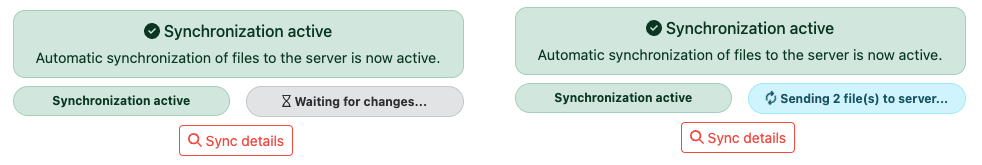
\includegraphics[width=0.9\textwidth]{imagenes/utilizadas/4-3-implementacion/rf11-1.png}
    \caption{Captura de las señales de sincronización activa y estado de la sincronización de ejercicios en progreso.}
    \label{fig:reqf11-1}
\end{figure}

El segundo elemento es el botón ``Sync details'' (detalles de la sincronización) que se muestra debajo del estado de la sincronización en cada ejercicio (visible en la \referenciaFigura{fig:reqf11-1}). Cuando se pulsa, se despliega un modal que contiene una lista con el histórico de los diez ficheros sincronizados más recientemente, los diez siguientes ficheros que serán sincronizados y el que está siendo transmitido al servidor en el momento presente, que dispone de una barra de progreso indicativa del avance de la operación.

La \referenciaFigura{fig:reqf11-2} muestra dos ejemplos de este modal: uno durante la sincronización de un fichero muy pesado (arriba) y otro que refleja la sincronización de una ingente cantidad de ficheros (abajo), constando de una lista de más de 150 ficheros sincronizados y de más de 300 ficheros pendientes de sincronizar. Para cada fichero sincronizado o pendiente de subir, se incluyen dos iconos: uno para reflejar el estado de la subida (rojo si está pendiente, amarillo si está en progreso y verde si se finalizó) y otro que indica el tipo de sincronización, pudiendo tratarse de la creación de un fichero (verde), una modificación de un fichero previamente existente (amarillo) o una eliminación (rojo). Los renombramientos aparecen como eliminaciones y nuevas creaciones.

\begin{figure}[ht]
    \centering
    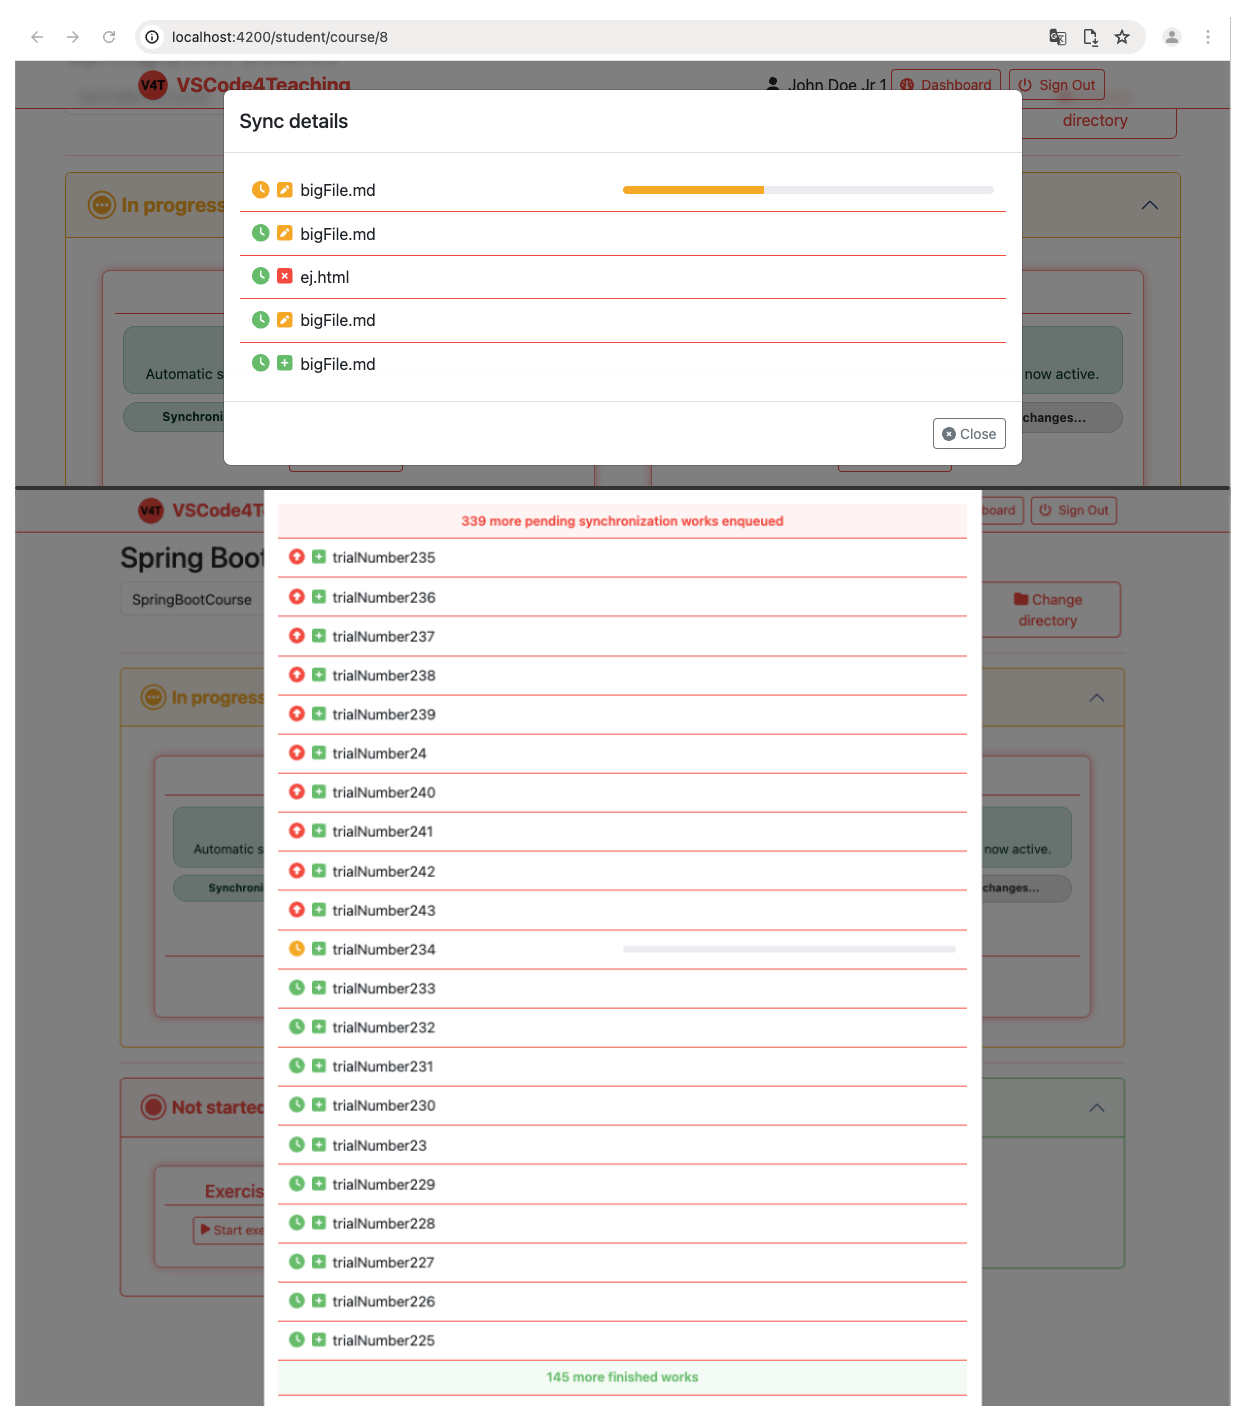
\includegraphics[width=0.8\textwidth]{imagenes/utilizadas/4-3-implementacion/rf11-2.png}
    \caption{Captura del modal explicativo de la sincronización de ficheros de un ejercicio.}
    \label{fig:reqf11-2}
\end{figure}

El diseño e implementación del algoritmo destinado a los procesos automáticos de cotejamiento y sincronización de cada ejercicio en progreso queda desarrollado pormenorizadamente en el \referenciaAnexo{anx:bajoNivelRF11}.

\subsubsection{\texttt{RF-12}: marcado de ejercicio como finalizado}
\label{subsec:rf12}

Tal como introduce el \referenciaConTT{subsec:rf9}{RF-9}, los estudiantes disponen de la capacidad para visualizar el detalle de los cursos en los que están matriculados al seleccionar un directorio local, pudiendo ver los ejercicios que los componen, en qué etapa del progreso de su realización se encuentran y realizar distintas acciones con ellos según su estado: mientras que los no comenzados únicamente pueden ser iniciados y pasan al estado ``en progreso'' (\referenciaConTT{subsec:rf10}{RF-10}), los ejercicios que se están realizando y sincronizando en tiempo real pueden ser finalizados. Para ello, los estudiantes pueden pulsar el botón ``Finish exercise'' (finalizar ejercicio) que aparece en la parte inferior de cada uno de los ejercicios en progreso, tal como sucede en la \referenciaFigura{fig:reqf9-1} con los ejercicios ``Exercise 1'' y ``Exercise 4''.

Una vez acometida esta acción sobre un ejercicio, se guardará como finalizado, trasladándose en la interfaz de usuario al área destinada a mostrar estos ejercicios (panel sombreado en verde con título ``Finished''). Esta acción comportará, además, la parada de la sincronización automática, ya que los ejercicios finalizados no pueden ser modificados, consolidando su último punto de progreso sincronizado en el servidor como propuesta final del estudiante para la resolución del ejercicio.

% \begin{figure}[ht]
%     \centering
%     \includegraphics[width=0.8\textwidth]{imagenes/utilizadas/4-3-implementacion/rf12-1.png}
%     \caption{Visualización del estudiante tras .}
%     \label{fig:reqf12-1}
% \end{figure}


\subsection{Requisitos no funcionales}
\label{subsec:reqsNoFuncionales}
\subsubsection{\texttt{RN-1}: aviso a usuarios con navegadores no compatibles con la \textit{File System Access API}}
\label{subsec:rn1}

Tal como se introduce en la \referenciaSeccion{subsec:tecFSA}, la aplicación web hace uso de la \textit{File System Access API}, que es la interfaz que permite que la aplicación web interactúe bidireccionalmente con las carpetas y ficheros del sistema local escogidos por los usuarios. Uno de sus mayores inconvenientes es la divergencia en su compatibilidad, ya que algunos navegadores no implementan esta interfaz, por lo que no permiten esta interacción.

Como consecuencia, algunos de los principales procesos de negocio incorporados en \textit{VSCode4Teaching}, tales como la descarga bajo demanda de los ficheros de las propuestas de los estudiantes por parte de los docentes (\referenciaConTT{subsec:rf4}{RF-4}) o, en el caso de los alumnos, la obtención de los ficheros de sus ejercicios (\referenciaConTT{subsec:rf10}{RF-10}) y la sincronización automática de las modificaciones registradas en los ejercicios durante su realización por parte de los estudiantes (\referenciaConTT{subsec:rf11}{RF-11}), no pueden ser realizados en navegadores no compatibles, mientras que el resto de procesos ya incorporados a la aplicación sí pueden ejecutarse, ya que no dependen del uso de la interfaz para la interacción con el sistema local de ficheros.

Para mejorar la interacción del usuario con la aplicación, este requisito establece la necesidad de informar desde el inicio a los usuarios autenticados acerca de la incompatibilidad de su navegador con la API en caso de acceder mediante, por ejemplo, Firefox o Safari, los navegadores más populares que no soportan esta característica. Con este fin, se introduce en todas las pantallas de la aplicación un aviso, tal como muestra la \referenciaFigura{fig:reqn1-1}, que aconseja el uso de un navegador compatible para poder aprovechar la completitud de las características de la aplicación.

\begin{figure}[ht]
    \centering
    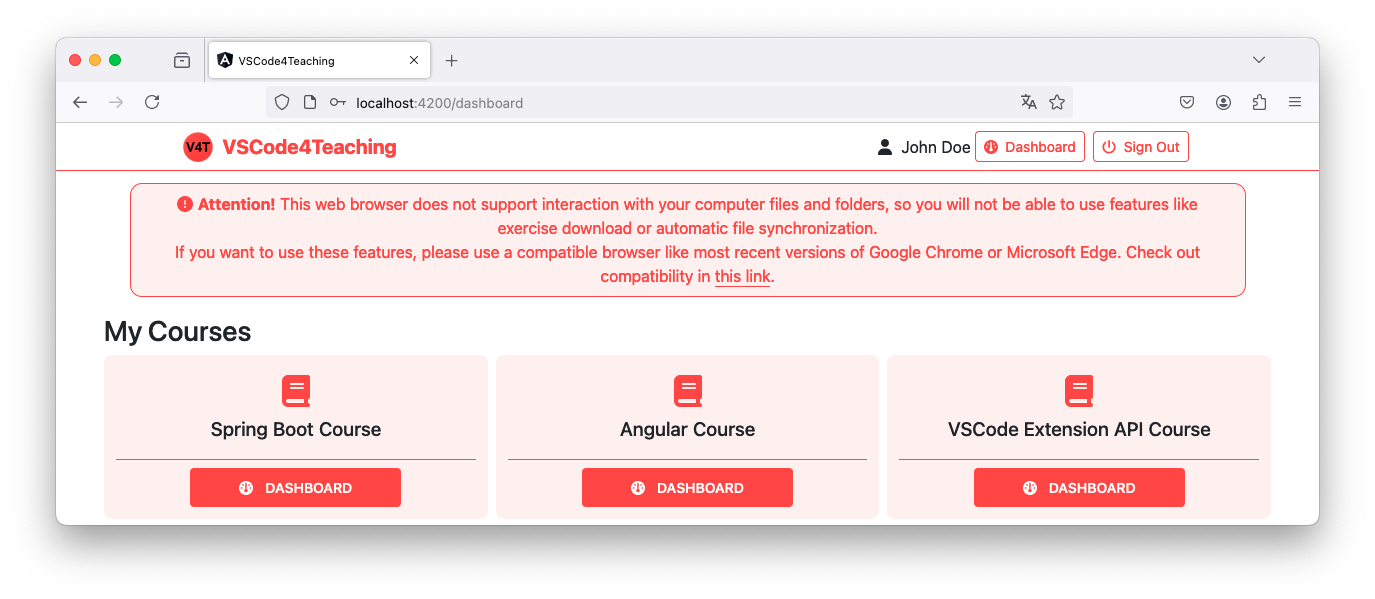
\includegraphics[width=\textwidth]{imagenes/utilizadas/4-3-implementacion/rn1-1.png}
    \caption{\textit{Dashboard} inicial de docentes en Firefox con aviso de incompatibilidad para el uso de la \textit{File System Access API}.}
    \label{fig:reqn1-1}
\end{figure}

\subsubsection{\texttt{RN-2}: aspecto visual de la aplicación web y coherencia entre interfaces}
\label{subsec:rn2}

El diseño de la interfaz de usuario de la nueva aplicación web aspira a ser coherente con la estética que venía empleándose en la extensión para Visual Studio Code, pretendiendo formar un entono familiar para quien ya utilizase la extensión de \textit{VSCode4Teaching} para Visual Studio Code.

La \referenciaFigura{fig:reqn2-1} muestra los dos \textit{dashboards} para el seguimiento del progreso de los ejercicios existentes: el de la extensión (abajo), que no se ha visto modificado y ya existía; y el de la aplicación web (arriba), que, inspirado en el diseño anterior, refleja la misma información haciendo uso de elementos gráficos de similar índole, ya que emplea el mismo esquema cromático y los mismos iconos informativos.

Esto también se observa en la \referenciaFigura{fig:reqn2-2}, que permite observar que los iconos empleados para la distinción de las tipologías de ejercicios son los mismos y que los dispuestos para las acciones de gestión de matriculados, compartición y adición de ejercicios son muy similares, potenciando la familiaridad del entorno a los usuarios.

\begin{figure}[!p]
    \centering
    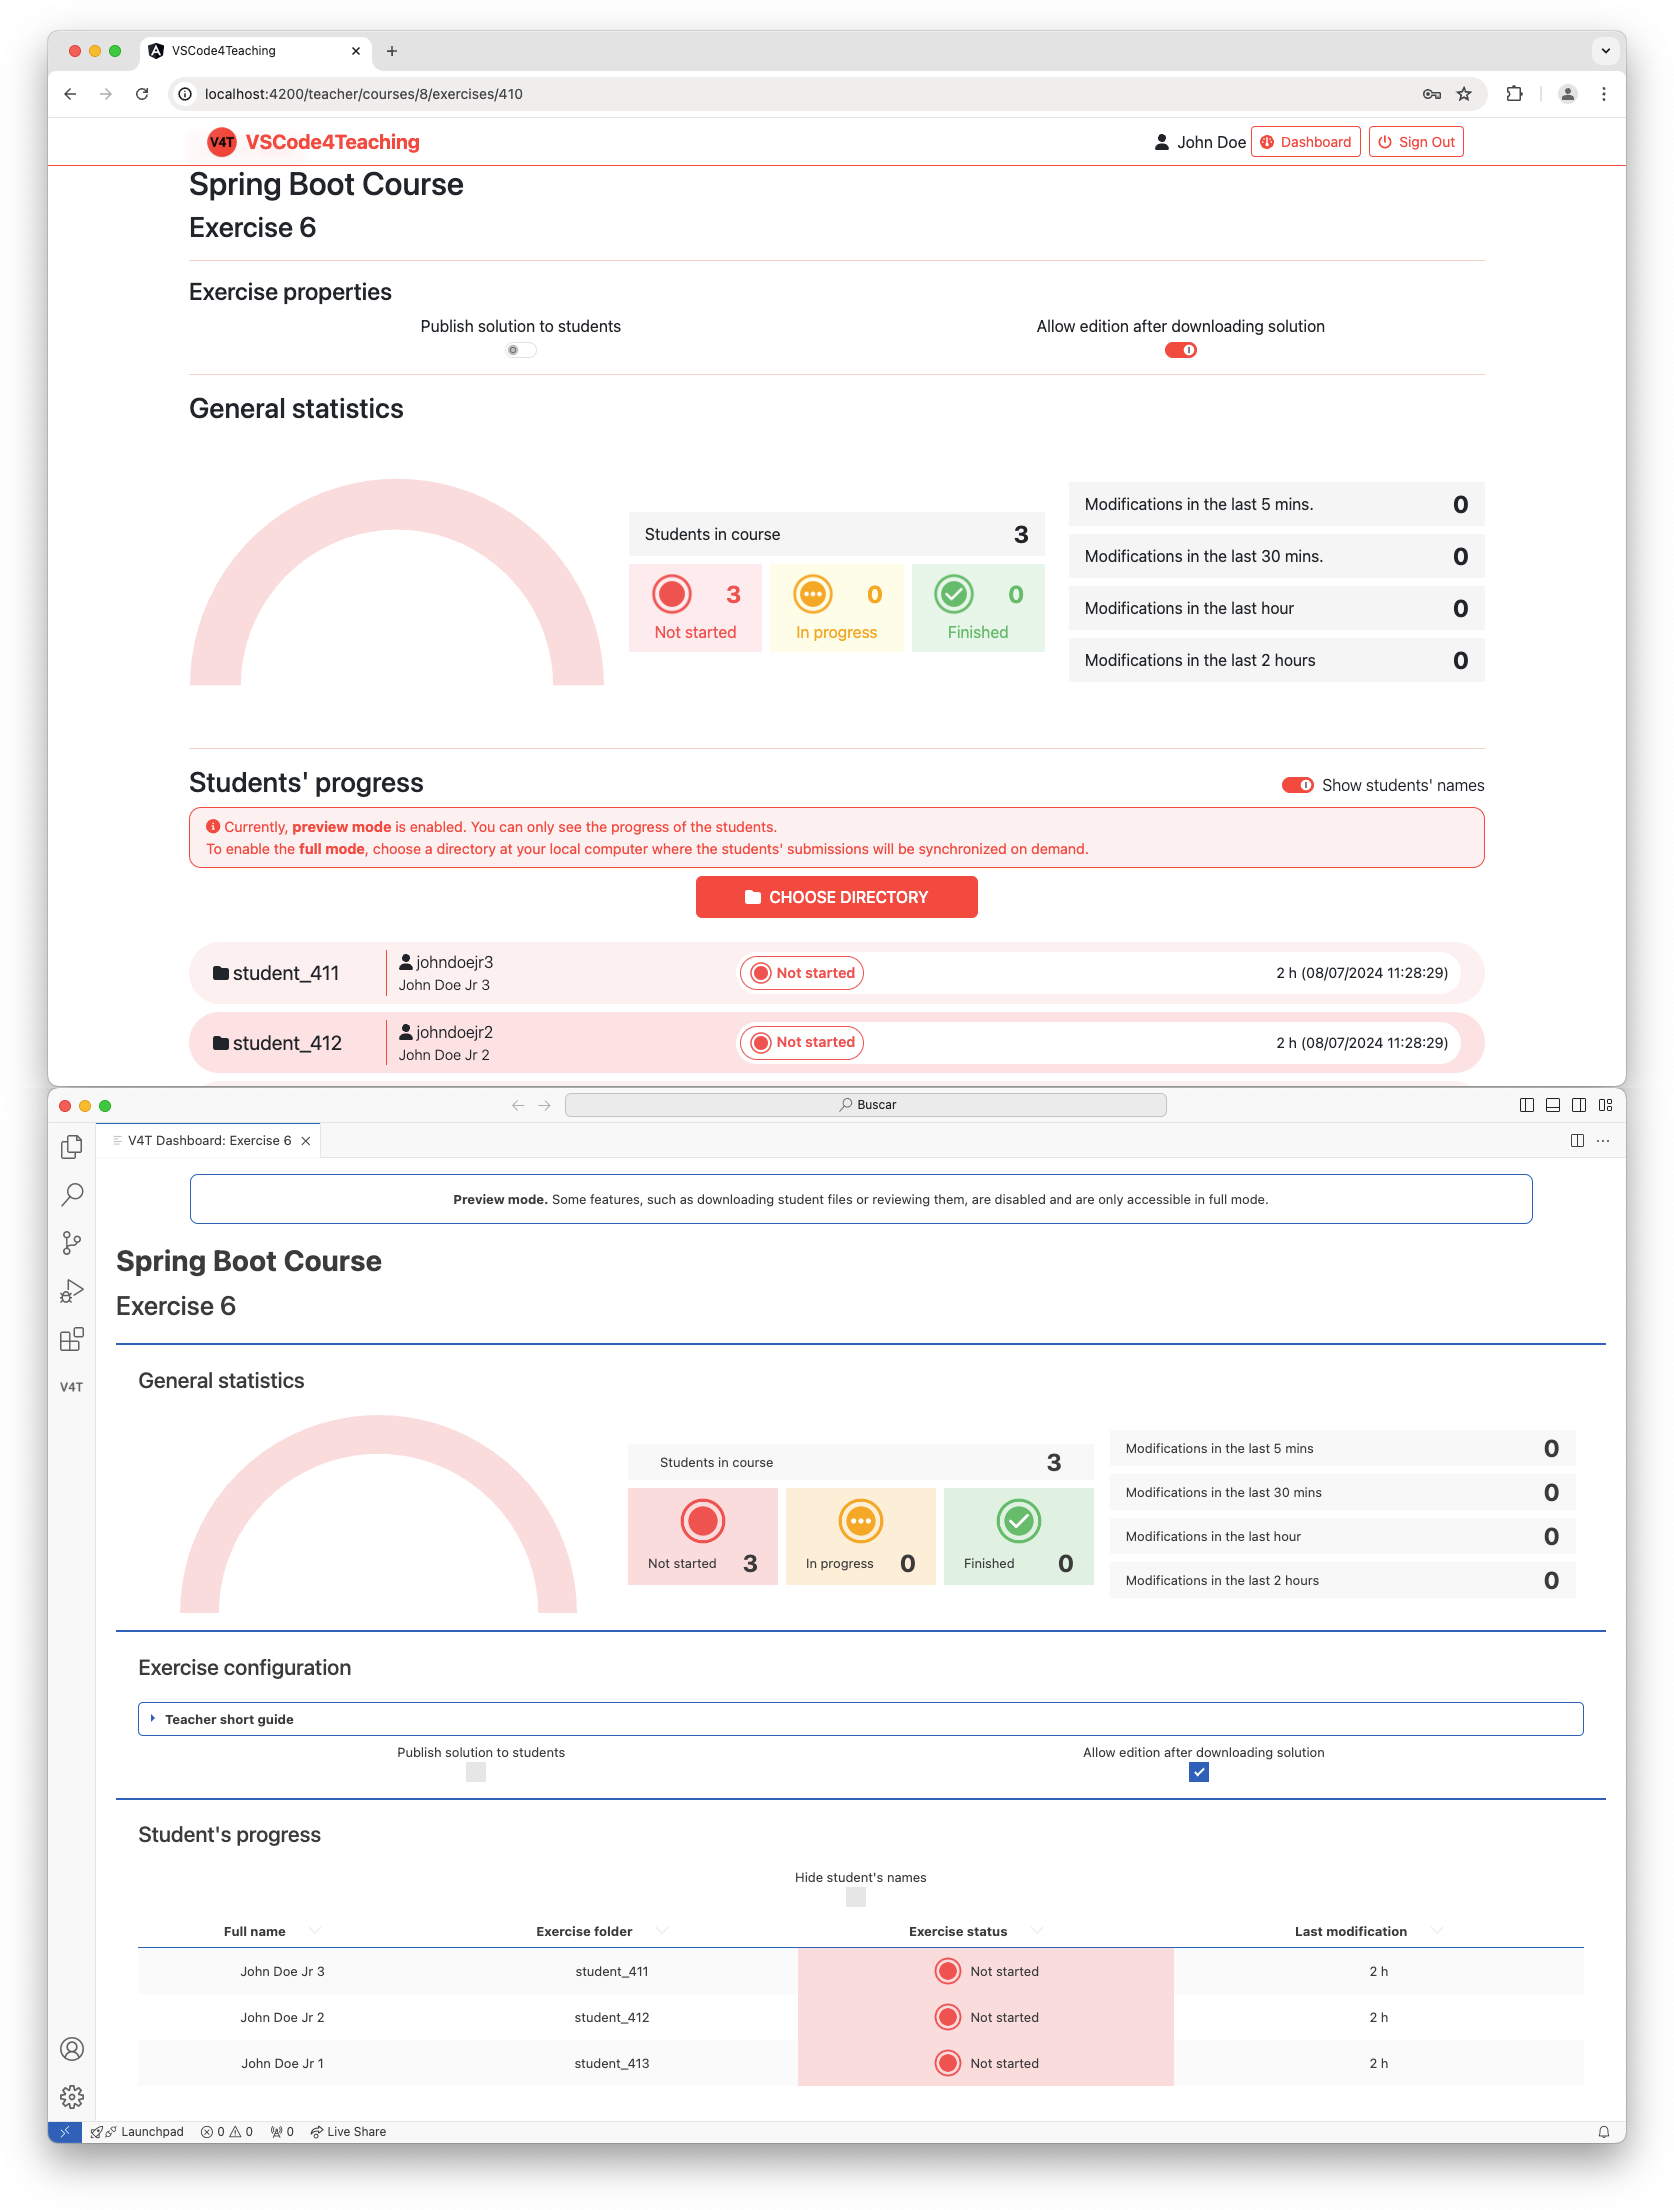
\includegraphics[width=\textwidth]{imagenes/utilizadas/4-3-implementacion/rn2-1.png}
    \caption{\textit{Dashboard} de un mismo ejercicio capturados a la vez en la aplicación web (arriba) y en la extensión para Visual Studio Code (abajo).}
    \label{fig:reqn2-1}
\end{figure}

\begin{figure}[ht!]
    \centering
    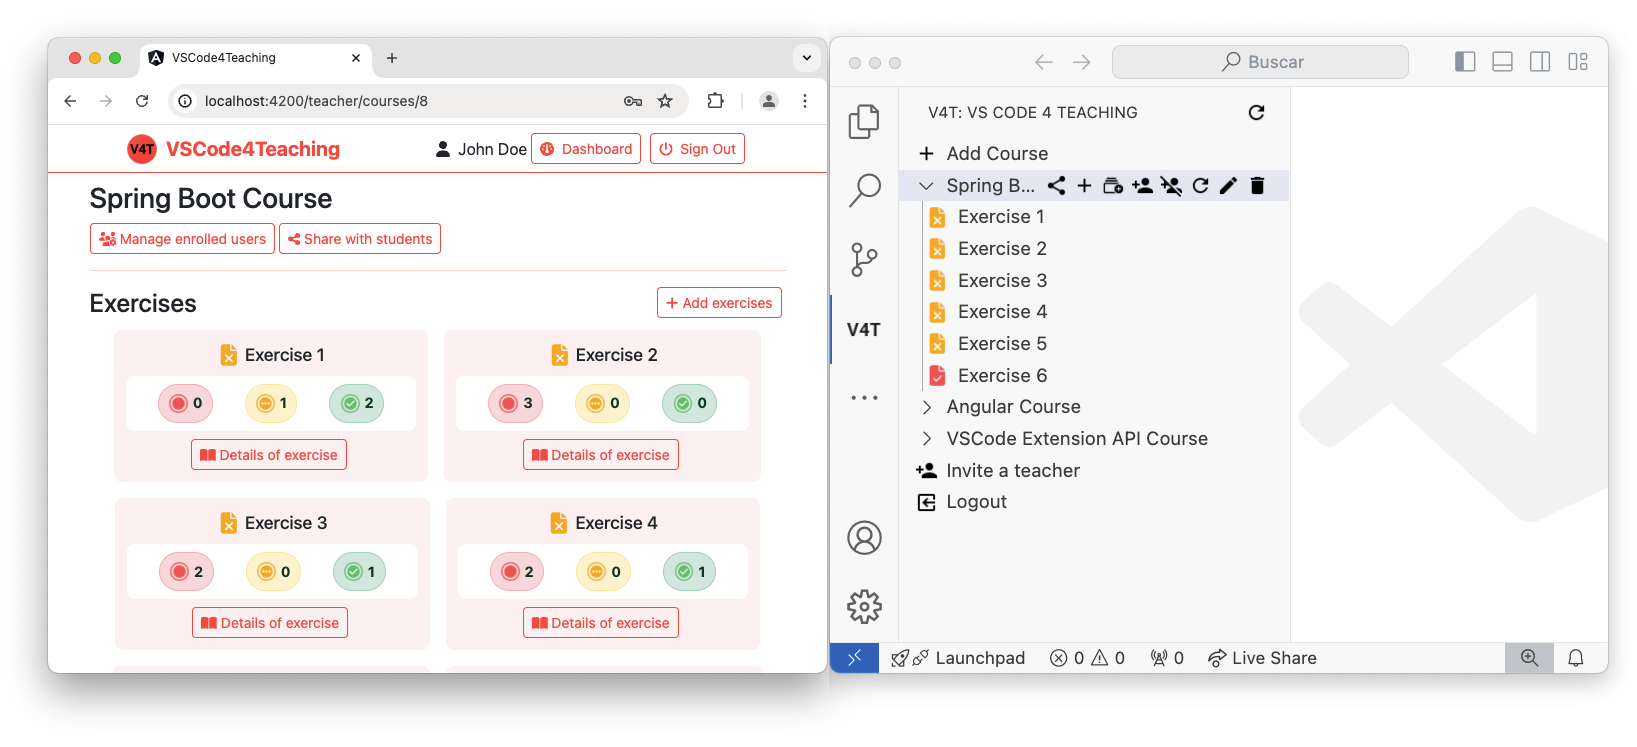
\includegraphics[width=\textwidth]{imagenes/utilizadas/4-3-implementacion/rn2-2.png}
    \caption{Comparativa entre los formatos empleados para mostrar a los docentes los ejercicios y configuraciones de las que disponen sus cursos.}
    \label{fig:reqn2-2}
\end{figure}

\subsubsection{\texttt{RN-3}: encriptación de \textit{tokens} JWT para autenticación}
\label{subsec:rn3}

El servidor de \textit{VSCode4Teaching} es \textit{stateless}; es decir, no almacena información sobre las interacciones realizadas por los usuarios con objeto de condicionar las siguientes, sino que cada una de las peticiones realizadas debe ser autocontenida e incluye en sí misma mediante sus cabeceras y cuerpo (si lo tiene) todo aquello que se debe tener en cuenta para proporcionar una respuesta, de modo que ninguna respuesta dependerá de las peticiones anteriormente realizadas \cite{Stateless}.

Si \textit{VSCode4Teaching} verifica esta característica es porque emplea \textit{tokens} JWT (siglas de \textit{JSON web token}, del inglés ``\textit{token} web en JSON'') para la autenticación de los usuarios. Estos \textit{tokens} son piezas de información representadas como cadenas de caracteres que permiten autenticar a los usuarios de forma autocontenida, ya que incluyen en sí mismos un \textit{payload} o carga útil que recoge qué usuario es el que está realizando una determinada petición. Se generan durante el inicio de sesión y quedan firmados mediante una clave privada, por lo que la suplantación de un usuario mediante un \textit{token} distinto del expedido durante la autenticación es inviable.

Sobre este mecanismo de autenticación preexistente, el presente requisito implementa el soporte a \textit{tokens} que, una vez generados, son encriptados nuevamente mediante un cifrado simétrico para añadir una capa adicional de seguridad. Este nuevo cifrado permite obtener cadenas no directamente comprensibles como \textit{tokens} JWT, añadiendo al servidor la lógica necesaria para manejar la presencia de cabeceras personalizadas llamadas \texttt{Encrypted-Authorization} en las peticiones procedentes de la aplicación web mediante la API REST y, además, como parámetro en la llamada inicial de las conexiones mediante \textit{Web Socket}.

\subsubsection{\texttt{RN-4}: adaptación de generación de imágenes Docker a nueva arquitectura}
\label{subsec:rn4}

El proyecto \textit{VSCode4Teaching} ya contaba previamente con la capacidad ejecutar su servidor a través de una imagen Docker, embebiendo en él la aplicación web Angular auxiliar como recurso estático. Además, se disponía de un fichero en formato YAML\footnote{YAML. Siglas de ``otro lenguaje de marcado más'' (del inglés \textit{Yet Another Markup Language}). Es un lenguaje de marcado de fácil lectura y comprensión que se aprovecha de la indentación para la jerarquización de declaraciones.}, \textit{docker-compose.yml}, para la orquestación de esta imagen con un contenedor para el sistema de persistencia basado en MySQL mediante Docker Compose.

Aunque la arquitectura del proyecto no ha variado al ejecutar la evolución realizada en este Trabajo Fin de Grado, se confiere mayor importancia a la aplicación web, que ahora busca ser sustitutiva o complementaria a la extensión para Visual Studio Code. La aplicación web auxiliar empleada anteriormente quedaba desplegada en el servidor en la ruta \texttt{/app}. Para mostrarla directamente al acceder a la raíz y, además, hacerla completamente compatible con el sistema de \textit{routing} propio de Angular (más información en la \referenciaSeccion{subsec:tecAngular}), se ha modificado el formato del despliegue e introducido un nuevo interceptor en el servidor que actúa como \textit{middleware}; esto es, como una capa intermedia de lógica ejecutada antes que el cotejamiento de rutas del servidor que tiene como finalidad detectar si las peticiones entrantes deben ser respondidas por el propio servidor o si deben ser derivadas a la aplicación web Angular para que esta, a través de su propia lógica de enrutamiento, ofrezca como respuesta los recursos gráficos necesarios.

Esta modificación de la lógica ha permitido preservar el método previamente empleado para la generación de la imagen Docker del servidor y la aplicación web. Esta configuración está alojada en el fichero \textit{Dockerfile} situado en la raíz del proyecto, en el que se define la construcción de la imagen en formato \textit{multi-stage}\footnote{\textit{Multi-stage}. Del inglés ``múltiples etapas'', se dice que un fichero de configuración es \textit{multi-stage} cuando se ejecutan varias fases en contenedores aislados y diferentes para dar lugar a una imagen final \cite{DockerfileMultistage}.}, articulándola en tres pasos ejecutados secuencialmente, tal como evidencia el \referenciaCodigo{cod:dockerfile}: compilación de la aplicación Angular en un contenedor Node, dando lugar a sendos recursos estáticos, compilación del servidor en un contenedor Maven (junto con los ficheros estáticos obtenidos en el paso anterior, que quedan copiados dentro del directorio del servidor destinado a este tipo de recursos) y generación de la imagen final sobre una base JDK que permite ejecutar la aplicación Java compilada en el paso anterior.

\begin{lstlisting}[language=Dockerfile,caption={Fichero \textit{Dockerfile} del proyecto, encargado de definir el proceso de generación de la imagen Docker del servidor y la aplicación web.},label=cod:dockerfile]
FROM node:18 AS angular
COPY vscode4teaching-webapp /usr/src/app
WORKDIR /usr/src/app
RUN ["npm", "install"]
RUN ["npm", "run", "build"]

FROM maven:3.9.7-eclipse-temurin-11 AS builder
COPY vscode4teaching-server /data
COPY --from=angular /usr/src/app/dist/vscode4teaching /data/src/main/resources/static/
WORKDIR /data
RUN ["mvn", "clean", "package"]

FROM eclipse-temurin:11
COPY --from=builder /data/target/vscode4teaching-server-*.jar ./app/vscode4teaching-server.jar
EXPOSE 8080
ENTRYPOINT [ "java", "-jar", "./app/vscode4teaching-server.jar" ]
\end{lstlisting}

Además, se ha ejecutado un cambio de localización de ficheros: la definición de Docker Compose, \textit{docker-compose.yml}, y el que contiene las variables de entorno que este último emplea (\textit{.env}) se han trasladado a la raíz del proyecto, donde ya se localizaba previamente el \textit{Dockerfile}.

Anteriormente se introducía en la imagen Docker un \textit{script} de \textit{shell} para organizar la sincronización de dependencias: preguntaba cada cierto tiempo si se disponía de una conexión válida con el sistema de persistencia configurado y solo cuando esta condición se cumplía, el \textit{script} lanzaba la ejecución del servidor, que requiere necesariamente disponer de la base de datos configurada desde su mismo inicio. Esta implementación se ha visto reemplazada por el uso del mecanismo de \textit{healthcheck}, que es una comprobación declarada como parte de la imagen empleada para la ejecución del contenedor de la base de datos, de modo que se relega en Docker Compose la responsabilidad de orquestar el funcionamiento de ambos contenedores. El \referenciaCodigo{cod:dockerCompose} muestra un fragmento del fichero \textit{docker-compose.yml} en el que se configura la dependencia entre contenedores y el mecanismo de espera mediante esta comprobación: la aplicación declara ser dependiente de la base de datos (\texttt{depends-on}), por lo que Docker Compose no ejecutará este contenedor hasta que la base de datos esté ``sana'', introduciendo en su configuración el mecanismo para comprobar cuándo este contenedor alcanza esta condición tras su inicialización.

\begin{lstlisting}[language=YAML,caption={Fichero \textit{docker-compose.yml} empleado para la orquestación de la imagen Docker del servidor con un contenedor para la base de datos.},label=cod:dockerCompose]
name: vscode4teaching

services:
  app:
    image: vscode4teaching/vscode4teaching:latest
    depends_on:
      db:
        condition: service_healthy
    env_file:
      - path: .env
        required: true
    ports:
      - ${SERVER_PORT}:${SERVER_PORT}
    volumes:
      - ./volume-v4t:${V4T_FILEDIRECTORY}
    restart: on-failure:6
  db:
    image: mysql:8.4.0
    restart: on-failure:3
    environment:
      MYSQL_ROOT_PASSWORD: ${MYSQL_ROOT_PASSWORD}
      MYSQL_DATABASE: ${MYSQL_DATABASE}
      MYSQL_USER: ${SPRING_DATASOURCE_USERNAME}
      MYSQL_PASSWORD: ${SPRING_DATASOURCE_PASSWORD}
    volumes:
      - ./volume-mysql:/var/lib/mysql
    healthcheck:
      test: "mysqladmin ping -h 127.0.0.1 || exit 1"
      interval: 5s
      timeout: 5s
      retries: 5
\end{lstlisting}

\subsubsection{\texttt{RN-5}: migración a GitHub Actions del sistema de integración continua}
\label{subsec:rn5}

Previamente al inicio del presente Trabajo Fin de Grado, el proyecto \textit{VSCode4Teaching} hacía uso de un sistema de integración y despliegue continuos a través de \textbf{Travis CI} en el que recaían tres tareas: cada vez que se producían modificaciones en la rama \texttt{master}, se ejecutaban las pruebas automáticas de servidor y extensión y, además, se publicaban nuevas etiquetas de la imagen del servidor en el repositorio en Docker Hub.

Este sistema se ha visto reemplazado por GitHub Actions, descrito en la \referenciaSeccion{subsec:herCiCd}. Sin embargo, esta migración no se ha limitado a replicar la funcionalidad previamente utilizada en el sistema de integración, entrega y despliegue continuos sino que, además, se ha aprovechado para ampliar su alcance.

Como consecuencia, el proyecto \textit{software} de \textit{VSCode4Teaching} cuenta ahora con dos flujos de trabajo (\textit{workflows}) diferenciados por componentes. El primero de estos, dedicado a las tareas relativas al servidor y la aplicación web, cuenta con tres trabajos definidos:
\begin{itemize}
    \item \texttt{Test}. Es el trabajo encargado de la ejecución de la batería de pruebas automáticas implementada en el servidor. Se ejecuta cada vez que se produce una alteración en las ramas \texttt{master} o \texttt{develop} del proyecto y, además, cuando se produce un \textit{pull request}\footnote{\textit{Pull request}. En su origen, solicitud realizada al propietario legítimo de un código para realizar una incorporación de otro código implementado fuera del repositorio original. Actualmente, además, se utiliza como sistema organizativo que permite coordinar la fusión de las distintas ramas de un repositorio y dotar a este proceso de un entorno que permite debates entre programadores, solicitar aprobaciones y ejecutar validaciones automáticas, entre otros.} entre ellas para conocer el estado de las pruebas antes de fusionar cambios a la rama del código de producción.
    \item \texttt{Publish}. Se encarga de la publicación de las nuevas versiones lanzadas al repositorio en Docker Hub y, por tanto, se ejecuta cada vez que se modifica la rama \texttt{master}. Genera una imagen Docker utilizando la declaración existente en el proyecto (véase la \referenciaSeccion{subsec:rn4}) y la publica en el repositorio del proyecto en Docker Hub, liberando dos etiquetas: actualiza la versión \textit{latest} de la imagen y, además, genera una nueva específica para la versión liberada.
    \item \texttt{Deploy}. Una vez publicada una nueva versión en Docker Hub, se accede mediante SSH\footnote{SSH. Siglas de ``terminal seguro'' (del inglés \textit{Secure SHell}). Es un protocolo utilizado para la administración remota de computadores.} a la máquina de producción, le transfiere una nueva versión del fichero Docker Compose en la que se utiliza la nueva versión puesta en producción, descarga la imagen desde Docker Hub y aplica los cambios al despliegue, dejando activa en producción la nueva versión automáticamente.
\end{itemize}

Análogamente, se declara un flujo de trabajo para la extensión que comprende únicamente los dos primeros trabajos descritos para el caso anterior, particularizándolos para la plataforma \textit{software} que emplea este componente. De este modo, para la extensión se ejecuta la batería de pruebas automáticas tras cada \textit{commit} en las ramas \texttt{master}, \texttt{develop} y cuando se produzca un \textit{pull request} entre ellas y, si se ha lanzado una nueva versión, se publica automáticamente en el Visual Studio Code Marketplace.

Todos los flujos anteriormente descritos quedan declarados en sendos ficheros YAML dentro del directorio \texttt{.github/workflows} en el proyecto, siendo esta la ubicación requerida por GitHub Actions para ejecutarlos automáticamente. Sirva como ejemplo el \referenciaCodigo{cod:ciGitHubTestServer}, que es la especificación para GitHub Actions del trabajo que ejecuta las pruebas automáticas del servidor, que es el primero de los especificados en el fichero \texttt{server.ci.yml}.

\begin{lstlisting}[language=YAML,caption={Fragmento del flujo de trabajo de acciones automáticas relativas a la integración continua del servidor.},label=cod:ciGitHubTestServer]
name: "Server pipeline"

on:
  push:
    branches:
      - master
      - main
      - develop
  pull_request:
    branches:
      - master
      - main
      - develop

jobs:
  test:
    runs-on: ubuntu-latest
    defaults:
      run:
        working-directory: ./vscode4teaching-server
    steps:
      - name: Checkout repository
        uses: actions/checkout@v4
      - name: Set up Java version
        uses: actions/setup-java@v4
        with:
          java-version: 11
          distribution: temurin
      - name: Test
        run: ./mvnw clean dependency:resolve test
  publish:
    if: ${{ github.event_name == 'push' && github.ref == 'refs/heads/main' }}
    needs: test
    # [...]   
  deploy:
    if: ${{ github.event_name == 'push' && github.ref == 'refs/heads/main' }}
    needs: publish
    # [...]
\end{lstlisting}

En la \referenciaFigura{fig:reqn5-1} se muestra una parte del histórico de ejecuciones de los flujos de trabajo definidos para varios \textit{commits} ejecutados sobre la rama \texttt{develop}. GitHub Actions posibilita acceder al detalle de cada ejecución, permitiendo visualizar gráficamente el estado y disposición de los trabajos realizados. Además, en caso de ser necesario, también se pueden obtener los registros en detalle de la ejecución de cada uno de los trabajos que componen un flujo.

\begin{figure}[h]
    \centering
    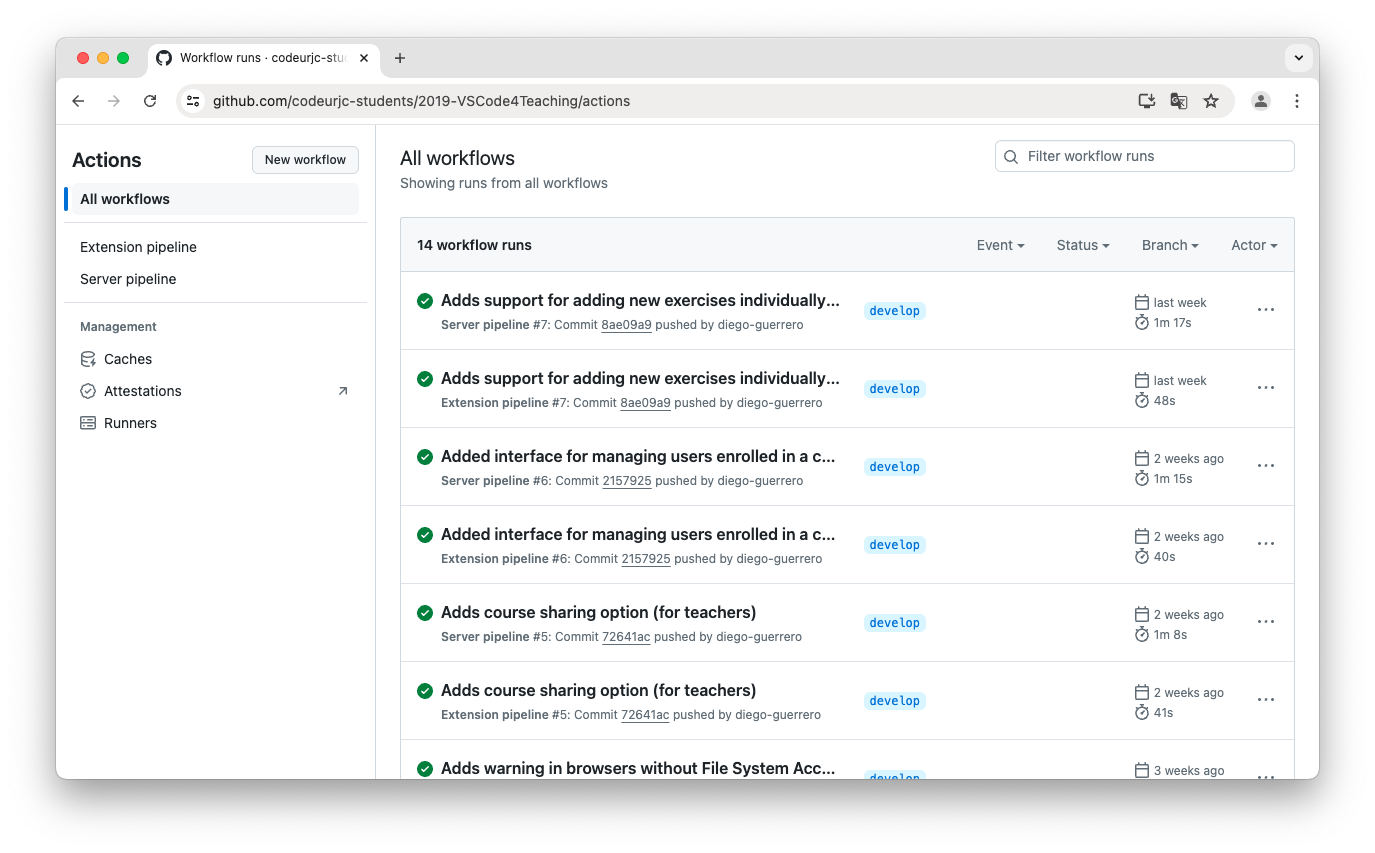
\includegraphics[width=\textwidth]{imagenes/utilizadas/4-3-implementacion/rn5-1.png}
    \caption{Fragmento del listado de ejecuciones de los flujos de trabajo de integración continua con GitHub Actions.}
    \label{fig:reqn5-1}
\end{figure}



% Sección 4.4: Pruebas
%  En esta sección se describen las pruebas automáticas que han sido implementadas para el proyecto. Sobre los tests,
%  conviene indicar la cobertura del código. Si no se han implementado pruebas automáticas, deberían haberse
%  implementado y describirse aquí o tener una buena justificación de por qué no se han implementado.
\section{Verificación de \textit{software} y funcionalidad}
\label{sec:verificacion}
Muchos teóricos de la ingeniería del \textit{software} afirman que la verificación del código mediante pruebas es indispensable para poder garantizar su calidad. Por ejemplo, Robert C. Martin afirma que ``las pruebas unitarias son necesarias para garantizar que el código es flexible, mantenible y reutilizable, ya que eliminan el miedo a hacer modificaciones en el código'' \cite{CleanCode}.

La nueva aplicación web implementada durante el presente hito evolutivo de \textit{VSCode4Teaching} no incluye pruebas automáticas, ya que se ha primado alcanzar una versión funcional de la aplicación por encima de la verificación de su comportamiento, que requerirá de la implementación de pruebas de tres tipos: unitarias, para corroborar el funcionamiento de la lógica de negocio; de integración, para la comprobación de la correcta comunicación con el servidor; y \textit{end-to-end} o de interfaz, con el fin de verificar que la interfaz de usuario se adecía a los requerimientos específicos de cada situación; pudiendo verse complementadas por otros tipos de pruebas, como las de carga o rendimiento, las de accesibilidad o las pruebas de funcionamiento en múltiples navegadores, especialmente importantes en este caso por las divergencias de compatibilidad de las tecnologías empleadas. La incorporación de pruebas automáticas para la garantía de la calidad de la aplicación web es uno de los primeros trabajos a futuro del proyecto, tal como recoge la \referenciaSeccion{subsec:trabajosFuturos}.

El servidor y la extensión cuentan con pruebas automáticas implementadas. Estas pruebas se basan en el uso de aserciones, que son comparaciones entre los valores obtenidos al ejecutar las pruebas y los valores deseados; y en dobles, que son piezas \textit{software} que permiten sustituir las dependencias empleadas que queden fuera del ámbito de la prueba realizada para simular su comportamiento en un escenario real y poder ejecutar la prueba al completo proporcionando valores conocidos a la salida de la dependencia reemplazada.

Las pruebas implementadas son de dos tipos: unitarias, que son aquellas que tienen como alcance una sola capa del \textit{software} y que emplean dobles para simular el funcionamiento de sus dependencias; y de integración, que verifican cómo interactúan entre sí las distintas capas del mismo componente o cómo se produce la comunicación entre el componente verificado y otros agentes \textit{software}.

\subsection{Pruebas automáticas del servidor}
\label{subsec:testingServidor}
Tal como consta en la \referenciaSeccion{subsec:tecServidor}, el servidor hace uso de JUnit para la implementación y ejecución de las pruebas automáticas implementadas en el servidor. Esta biblioteca incorpora una amplia cantidad de aserciones y permite generar dobles de dependencias de forma sencilla para el implementador. El servidor incluye \textit{tests} de tres tipos:
\begin{itemize}
    \item Pruebas sobre controladores. Incluidas en el paquete \texttt{controllertests}, son pruebas unitarias que verifican el correcto funcionamiento de la capa de los controladores REST de Spring y que se implementan ejecutando llamadas HTTP a la aplicación y utilizando dobles que suplantan el funcionamiento de los servicios que emplean para la generación de la respuesta.
    \item Pruebas sobre servicios. Localizadas en el paquete \texttt{servicetests}, son pruebas unitarias que buscan verificar el correcto funcionamiento de la capa de los servicios Spring, que es la que incluye la traslación al \textit{software} de la lógica de negocio, y se implementan mediante la suplantación con dobles de los DAO de la aplicación, proporcionando instancias basadas en un conjunto de valores conocidos.
    \item Pruebas de integración. Ubicadas en el paquete \texttt{integrationtests}, y al contrario que las anteriores, son pruebas que verifican el funcionamiento de la aplicación en su integridad, lanzando una petición HTTP y sin proporcionar ningún tipo de doble. Emplean un mecanismo para la inicialización de valores conocidos en una base de datos embebida en la aplicación e instanciada únicamente durante el lanzamiento de estas pruebas, hecho que posibilita la ejecución de pruebas que validan la correcta interacción entre las capas de la arquitectura y, además, con el sistema de persistencia.
\end{itemize}

Cuantitativamente, la batería de pruebas automáticas del servidor contiene un total de 96 pruebas que alcanzan un $78,3\%$ de las clases y un $79,4\%$ de los métodos que conforman este componente.

\subsection{Pruebas automáticas de la extensión}
\label{subsec:testingExtension}
Análogamente al caso anterior, y tal como enuncia la \referenciaSeccion{subsec:tecExtension}, la extensión para Visual Studio Code también incluye una batería de pruebas automáticas implementada sobre Jest que permite verificar el correcto funcionamiento de este componente en su integridad.

Las pruebas incorporadas a la extensión permiten verificar el correcto funcionamiento de su arquitectura en su práctica totalidad, para lo que incorpora 129 pruebas automáticas. Entre ellas, cabe reseñar una cobertura del código superior al $80\%$ sobre el cliente empleado para el intercambio de peticiones con el servidor, sobre algunos de los elementos empleados en la interfaz de usuario (como los elementos mostrados en la barra de actividad) y sobre el modelo del dominio. El dato de cobertura total de la extensión es de un $61,7\%$ de las líneas de código del proyecto y de un $54,9\%$ de las funciones que incorpora.


% Sección 4.5: Distribución y despliegue
\section{Distribución}
\label{sec:distribucion}
Se introduce a continuación la forma en que se divulga el proyecto \textit{VSCode4Teaching} en sus distintas etapas: tanto como código fuente (\referenciaSeccion{subsec:distribFuente}) como los artefactos construidos de la extensión y el servidor con la aplicación web (\referenciaSeccion{subsec:distribArtefactos}).

\subsection{Distribución del código fuente}
\label{subsec:distribFuente}
El código fuente del proyecto \textit{VSCode4Teaching} se encuentra íntegramente publicado en la red a través de un repositorio alojado en GitHub (\referenciaSeccion{subsec:tecGitHub}), tal como ilustra la \referenciaFigura{fig:distribGitHub}.

\begin{figure}[ht]
    \centering
    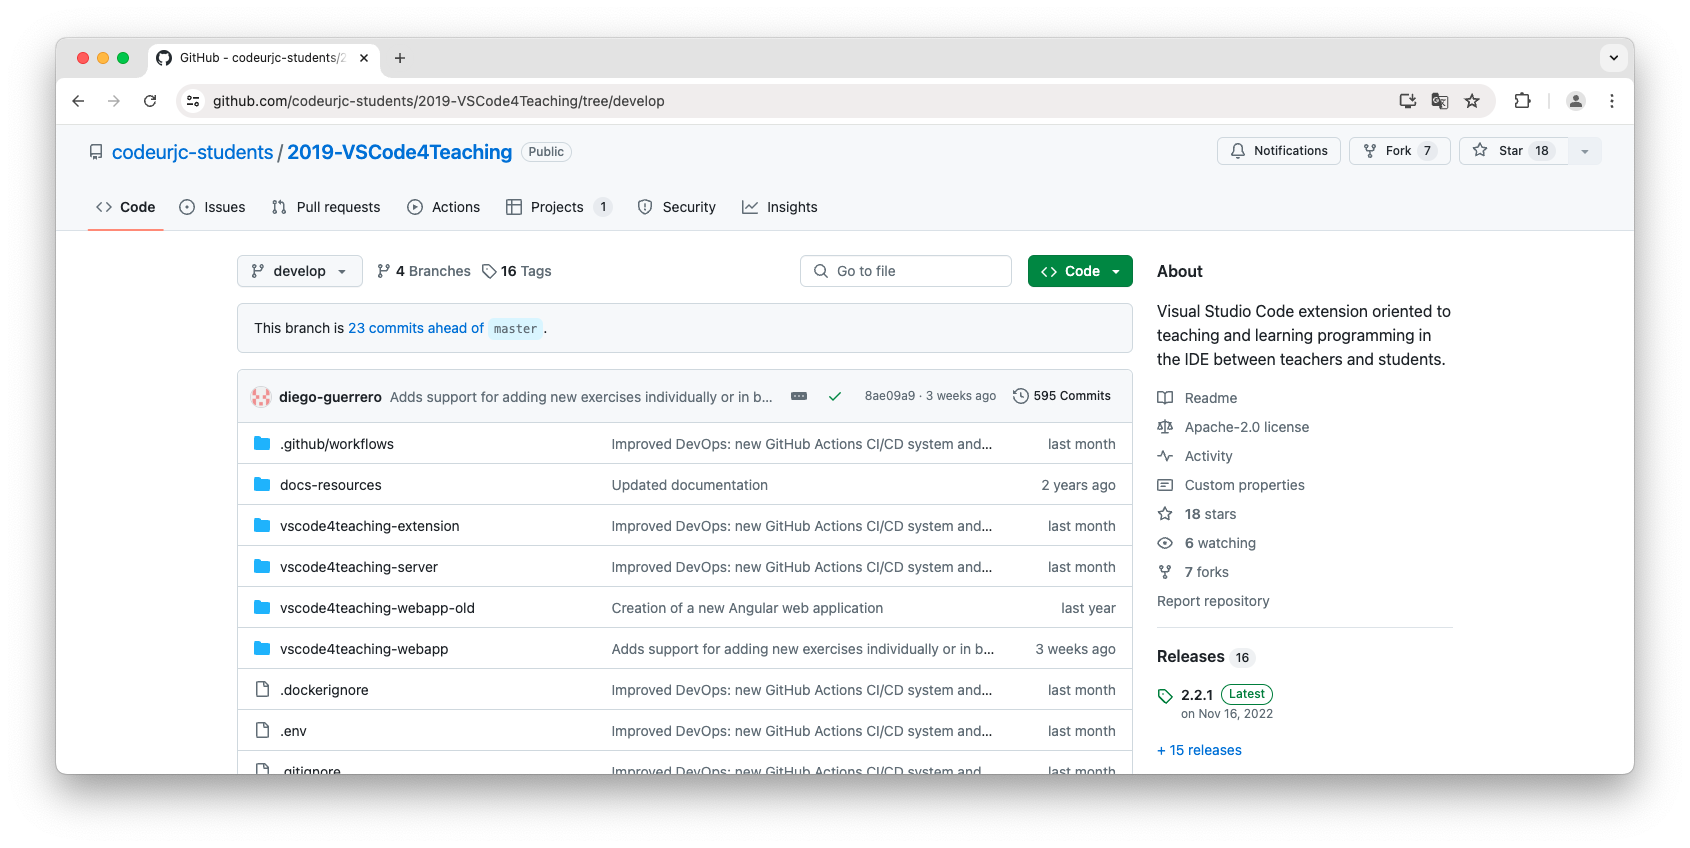
\includegraphics[width=0.8\linewidth]{imagenes/utilizadas/4-5-distribucion/repoGitHub.png}
    \caption{Repositorio en GitHub del proyecto \textit{VSCode4Teaching}.}
    \label{fig:distribGitHub}
\end{figure}

Este repositorio viene utilizándose desde el inicio del proyecto y contiene el histórico completo de cambios producidos en la aplicación durante su evolución. Se encuentra alojado en la siguiente dirección:

\vspace{-0.7\baselineskip}
\begin{center}
    \href{https://github.com/codeurjc-students/2019-VSCode4Teaching}{https://github.com/codeurjc-students/2019-VSCode4Teaching}.
\end{center}
\vspace{-0.7\baselineskip}

Tal como incluye en el fichero \texttt{LICENSE} alojado en su raíz, el código fuente de \textit{VSCode4Teaching} está sujeto a la licencia Apache License 2.0 \cite{ApacheLicense}. Esta licencia es permisiva y permite a otros desarrolladores utilizar el código del proyecto para su modificación y redistribución libremente siempre y cuando se mantenga la licencia sobre todas aquellas partes del fuente que no hayan sido adaptadas en las nuevas versiones generadas.

Esta licencia permite, además, aseverar que \textit{VSCode4Teaching} es \textit{software} libre, ya que otorga a sus usuarios las cuatro libertades esenciales: libertad de ejecutarlo como se desee y para lo que se desee, libertad de estudiar cómo funciona y poder adaptarlo para modificar su comportamiento, libertad para redistribuirlo y libertad para distribuir también las copias modificadas \cite{FreeSoftwareFreedoms}.

\subsection{Distribución de artefactos}
\label{subsec:distribArtefactos}
Además de la distribución de su código fuente, el proyecto \textit{VSCode4Teaching} publica sus artefactos empaquetados para una utilización directa más sencilla de la aplicación. Tal como se introduce en la \referenciaSeccion{subsec:tecDistrib}, se hace uso de dos repositorios públicos para la divulgación de la extensión para Visual Studio Code y del servidor empaquetado junto con la aplicación web en una imagen Docker (véase el requisito \referenciaConTT{subsec:rn4}{RN-4}).

La extensión queda publicada mediante el sistema de integración continua (véase el requisito \referenciaConTT{subsec:rn5}{RN-5}) en el Visual Studio Code Marketplace, lo que posibilita que esté disponible directamente para los usuarios a través de la herramienta integrada para la búsqueda e instalación de extensiones, tal como muestra la \referenciaFigura{fig:distribVSCodeMarketplace}.
\begin{figure}[ht]
    \centering
    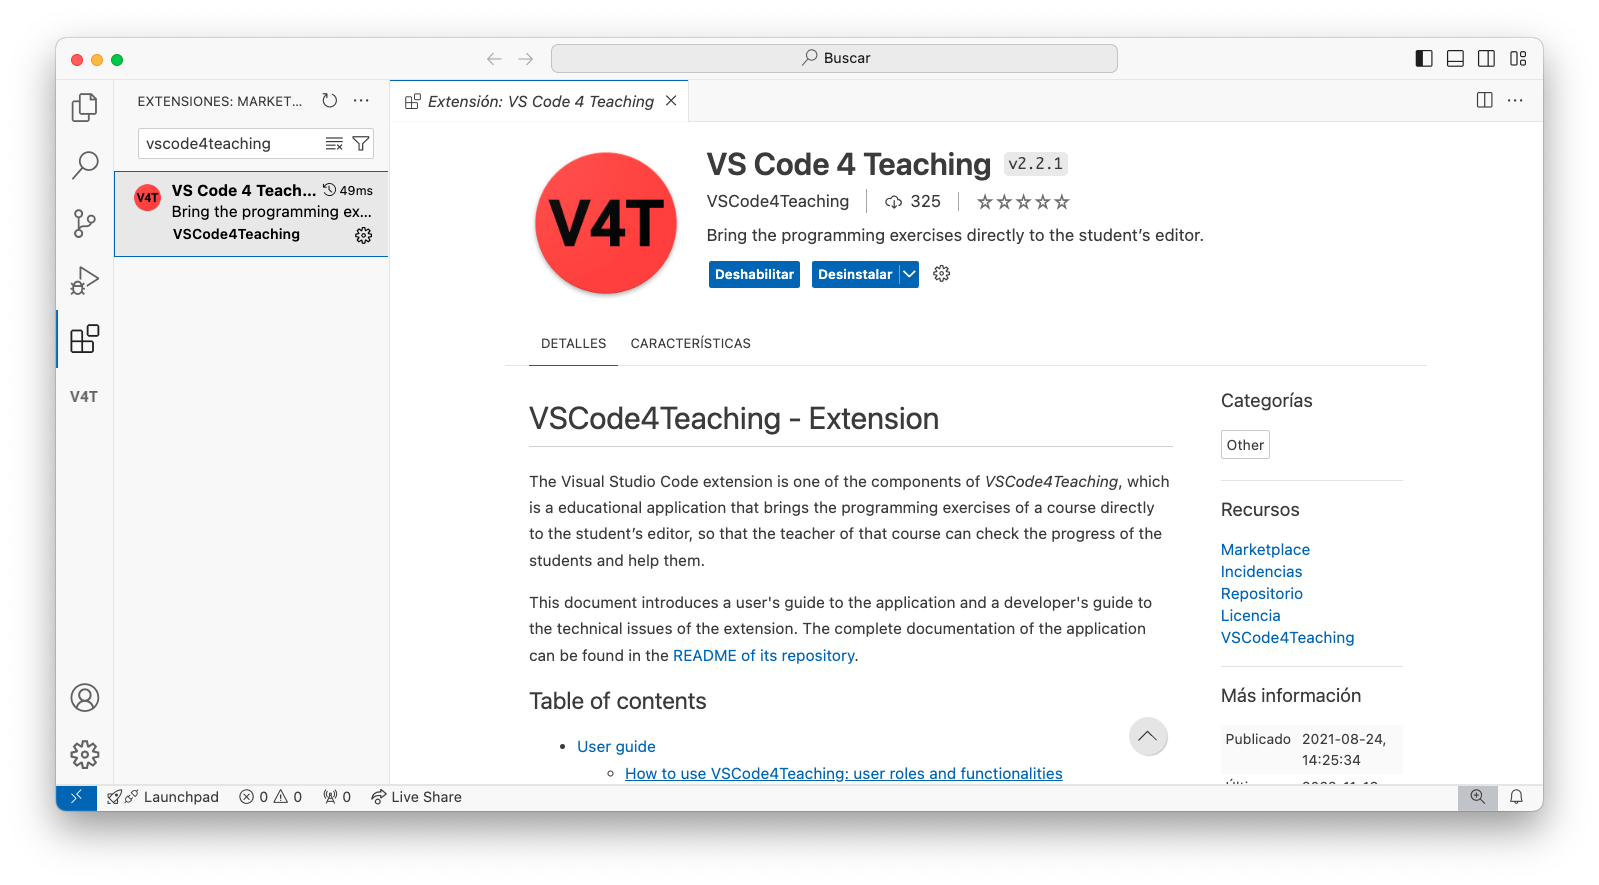
\includegraphics[width=0.8\linewidth]{imagenes/utilizadas/4-5-distribucion/vscodeMarketplace.png}
    \caption{Extensión de \textit{VSCode4Teaching} en el área de búsqueda y descarga de extensiones en Visual Studio Code.}
    \label{fig:distribVSCodeMarketplace}
\end{figure}

\noindent El enlace a la extensión publicada es el siguiente:
\vspace{-0.7\baselineskip}
\begin{center}
    \href{https://marketplace.visualstudio.com/items?itemName=VSCode4Teaching.vscode4teaching}{https://marketplace.visualstudio.com/items\\ ?itemName=VSCode4Teaching.vscode4teaching}.
\end{center}
\vspace{-0.7\baselineskip}

Por otro lado, el servidor queda empaquetado junto con la aplicación web como \textit{frontend} en una imagen Docker generada mediante el sistema de CI/CD que queda publicada en el Docker Hub, tal como se detalla en los requisitos \referenciaConTT{subsec:rn4}{RN-4} (acerca de la generación) y \referenciaConTT{subsec:rn5}{RN-5} (sobre la automatización), quedando disponible para su utilización mediante, por ejemplo, el fichero \textit{docker-compose.yml} disponible en el repositorio.

\noindent El enlace a la imagen publicada del servidor con la aplicación web es el siguiente:
\vspace{-0.7\baselineskip}
\begin{center}
    \href{https://hub.docker.com/r/vscode4teaching/vscode4teaching}{https://hub.docker.com/r/vscode4teaching/vscode4teaching}.
\end{center}
\vspace{-0.7\baselineskip}




% Sección 5: Conclusiones y trabajos futuros.

% Reflexión sobre el trabajo realizado, qué objetivos se han cumpliado y qué aspectos quedan pendientes para una
% futura ampliación del proyecto. Además se deben incluir unas conclusiones personales indicando lo que ha supuesto
% para el alumno la realización del trabajo.
% Extensión recomendada: entre 2 y 4 páginas.
\afterpage{\blankpage}
\chapter{Conclusiones y trabajos futuros}
\label{cap:conclusiones}

Esta última sección concluye el Trabajo Fin de Grado realizado, para lo que se analiza el cumplimiento de los objetivos estipulados ---\referenciaSeccion{subsec:cumplimientoObjetivos}---, se introducen varios posibles trabajos futuros de interés para el proyecto \textit{VSCode4Teaching} ---\referenciaSeccion{subsec:trabajosFuturos}--- e incluyendo, para finalizar, una opinión personal final acerca del Trabajo Fin de Grado ---\referenciaSeccion{subsec:aprendizajesPersonales}---.

\section{Cumplimiento de los objetivos estipulados}
\label{subsec:cumplimientoObjetivos}
El actual Trabajo Fin de Grado supone un cuarto hito evolutivo en el proyecto \textit{VSCode4Teaching}, basado en los objetivos iniciales estipulados recogidos en el \referenciaSeccion{cap:objetivos} sobre los que, a su vez, se asientan los requisitos especificados en la \referenciaSeccion{sec:requisitos} y cuyo diseño e implementación queda recogido en las subsiguientes secciones. Se confirma el cumplimiento de la totalidad de los objetivos establecidos, tal como se detalla a continuación:

\begin{itemize}
    \item El objetivo primero establece la necesidad de que los usuarios registrados puedan autenticarse (\referenciaConTT{subsec:rf1}{RF-1.1}) y, cuando hayan iniciado sesión de forma exitosa, puedan ver sus cursos matriculados, en el caso de los estudiantes; o impartidos, en el caso de los docentes, quienes también disponen de una visualización del detalle de un curso que refleja los ejercicios que contiene, aportando información básica adicional y acceso a las opciones de gestión del curso (\referenciaConTT{subsec:rf1}{RF-1.2}).
    
    Este objetivo también viene ratificado por la implementación del \referenciaConTT{subsec:rf9}{RF-9}, por el que los estudiantes disponen de una pantalla en la que, una vez elegido un directorio de su sistema local de ficheros, pueden visualizar con detalle el estado de ejecución de los ejercicios de sus cursos.
    Además, cabe reseñar la utilidad del requisito \referenciaConTT{subsec:rn2}{RN-2} en este objetivo, ya que proporcionar un aspecto visual coherente con la extensión para Visual Studio Code facilita a los usuarios previamente registrados la utilización y comprensión de la nueva aplicación web.
    \item El segundo objetivo especifica la necesidad de los docentes de disponer de la capacidad para añadir y gestionar los ejercicios de sus cursos. Este objetivo viene implementado por dos requisitos funcionales: \referenciaConTT{subsec:rf2}{RF-2}, por el que los docentes pueden añadir nuevos ejercicios en sus cursos de forma individual o en lotes de ejercicios con o sin propuesta de solución; y el \referenciaConTT{subsec:rf5}{RF-5}, que establece la necesidad de configurar la visibilidad de la solución propuesta por el profesor y la capacidad para realizar nuevas ediciones tras ser descargada por los estudiantes.

    Este objetivo, además, viene complementado por el \referenciaConTT{subsec:rn1}{RN-1}, por el que se muestra un aviso por pantalla en caso de utilizar un navegador no compatible con la interfaz para la interacción con los sistemas de ficheros locales, empleada para la creación de nuevos ejercicios.

    \item El objetivo tercero marca la necesidad de que los docentes dispongan de herramientas para el seguimiento en tiempo real del progreso de los estudiantes inscritos en sus cursos impartidos. Su intención queda materializada en la implementación de los requisitos \referenciaConTT{subsec:rn3}{RN-3}, por el que los docentes disponen de un \textit{dashboard} para cada ejercicio de sus cursos actualizado en tiempo real que contiene numerosas métricas acerca del progreso de los alumnos; y \referenciaConTT{subsec:rn4}{RN-4}, que añade a la interfaz anteriormente citada la posiblidad de elegir un directorio de sistema local de ficheros para descargar en él bajo demanda los ficheros que integran las propuestas de resolución de ejercicios de los estudiantes. Este último requisito conduce a la mención del valor aportado del requisito \referenciaConTT{subsec:rn1}{RN-1}, ya que la característica para la descarga no está disponible en navegadores no compatibles con la \textit{File System Access API}.

    \item El cuarto objetivo complementa las necesidades de los docentes en \textit{VSCode4Teaching} especificando la necesidad para la gestión de la matriculación de estudiantes en los cursos que imparten. Con este fin, el requisito \referenciaConTT{subsec:rf6}{RF-6} introduce la capacidad para la gestión de los estudiantes inscritos en los cursos a través de una interfaz visual que permite revocar inscripciones o matricular a nuevos usuarios. Adicionalmente, los docentes disponen de la capacidad para compartir un código único de inscripción asociado a sus cursos (\referenciaConTT{subsec:rf7}{RF-7}) que puede ser empleado por los estudiantes para su automatriculación (\referenciaConTT{subsec:rf8}{RF-8}).
    
    \item El objetivo quinto pone el foco en los estudiantes, quienes deben poder visualizar los ejercicios que componen sus cursos y realizarlos, sincronizando las modificaciones que realicen en sus propuestas de resolución. Este objetivo queda implementado a través de cuatro requisitos funcionales encadenados: la incorporación de la interfaz de usuario que permite a los estudiantes escoger un directorio del sistema de ficheros de su computador y obtener el detalle del progreso en la ejecución de los ejercicios del curso (\referenciaConTT{subsec:rf9}{RF-9}), poder descargar las plantillas iniciales de los ejercicios recién comenzados o el último punto de progreso sincronizado en el servidor en el directorio escogido (\referenciaConTT{subsec:rf10}{RF-10}), sincronizar automáticamente con el servidor el progreso de los ejercicios cada vez que se crea, modifica o elimina un fichero en el sistema local del estudiante (\referenciaConTT{subsec:rf11}{RF-11}) y otorgar a los estudiantes la capacidad para marcar sus propuestas de resolución como finalizadas, impidiendo nuevas ediciones (\referenciaConTT{subsec:rf12}{RF-12}). Cabe mencionar nuevamente la utilidad del requisito \referenciaConTT{subsec:rn1}{RN-1} y el valor que aporta a la ejecución exitosa del presente objetivo.
    
    \item El sexto objetivo hace énfasis en la calidad del proyecto, procurando la ejecución de actuaciones para la mejora de sus atributos de calidad. Entre las actuaciones realizadas, destaca la adición de una capa de seguridad extra en el mecanismo de autenticación (\referenciaConTT{subsec:rn3}{RN-3}), la adecuación de la generación de artefactos a la nueva arquitectura adoptada en el proyecto (\referenciaConTT{subsec:rn4}{RN-4}) y la mejora y automatización integral de los procesos de integración, entrega y despliegue continuos (\referenciaConTT{subsec:rn5}{RN-5}).
\end{itemize}

\section{Trabajos futuros: hoja de ruta del proyecto \textit{VSCode4Teaching}}
\label{subsec:trabajosFuturos}
\textit{VSCode4Teaching} es un proyecto que, tal como se refleja en la \referenciaSeccion{sec:cronologiaProyecto}, es el resultado de, junto con el presente, cuatro Trabajos Fin de Grado que marcan sobre él cuatro hitos evolutivos.

El actual Trabajo Fin de Grado no ha completado la migración de la extensión al formato de aplicación \textit{web}, aunque la funcionalidad principal de la aplicación ya puede ser ejecutada a través de esta nueva interfaz de usuario. La actual situación del proyecto permite plantear una extensa batería de posibles trabajos futuros de gran interés y valor para el usuario.

\noindent Para la mejora de la aplicación \textit{web} de \textit{VSCode4Teaching}, cabe considerar:
\begin{enumerate}
    \item Finalizar algunas de las características más complejas, tales como la gestión pormenorizada de cursos y ejercicios, así como perfeccionar el funcionamiento de las características existentes, realizando sobre la aplicación nuevos y constantes trabajos de mantenimiento correctivo y perfectivo.
    \item Incorporar la posibilidad de visualizar los contenidos de los ejercicios y de modificarlos a través de un editor de código integrado ligero que quede embebido en la aplicación \textit{web}. Aunque puede ser muy complejo dotar a la herramienta de la capacidad para ejecutar los proyectos de los alumnos, es interesante disponer un editor mínimamente interactivo que permita visualizar los contenidos de los ejercicios o hacer ediciones rápidas sobre ellos sin necesidad de utilizar un directorio en el sistema local de ficheros, permitiendo así, además, ver o editar ejercicios en navegadores no compatibles con la \textit{File System Access API}. Por ejemplo, el editor que emplea Visual Studio Code, llamado \textit{Monaco} \cite{MonacoEditor}, está disponible como \textit{software} libre bajo licencia MIT y puede ser integrado en cualquier aplicación \textit{web}.
    \item Implementar una amplia batería de pruebas automáticas de diversa índole: pruebas unitarias asociadas a la lógica de negocio, pruebas de integración para garantizar la correcta comunicación con el servidor y pruebas de sistema o \textit{end to end} (E2E) para ratificar el correcto funcionamiento de los elementos dispuestos en la interfaz de usuario y la adecuación de la implementación de los distintos procesos de negocio disponibles para los usuarios.
\end{enumerate}

Por otro lado, en el actual punto de evolución de \textit{VSCode4Teaching} como proyecto \textit{software}, cabe analizar si es pertinente continuar manteniendo la extensión para Visual Studio Code en paralelo a la aplicación \textit{web} y disponer de dos clientes plenamente funcionales disponibles para los usuarios. Esta decisión debe dirimirse tomando en consideración varios factores, entre los que cabe destacar la dificultad y el coste temporal que conlleva el mantenimiento paralelo de dos clientes con la misma funcionalidad y finalidad.

En particular, si se decidiese continuar manteniendo ambos clientes de forma paralela, podría ser interesante plantear una reestructuración de su código para abstraer la funcionalidad común a ambos componentes a una biblioteca propia del proyecto. Como ambos clientes se basan en la plataforma Node y en la gestión de paquetes realizada a través de NPM, tal como se detalla en la \referenciaSeccion{subsec:tecAppWeb} y la \referenciaSeccion{subsec:tecExtension}, puede resultar conveniente generar un paquete que abstraiga toda la lógica de negocio y la interacción con el servidor, que es compartida por ambas aplicaciones y que actualmente se realiza utilizando bibliotecas y mecanismos diferentes, logrando así eliminar gran parte de la duplicidad de código entre ambos clientes y, por tanto, facilitando el esfuerzo de mantenimiento, de modo que cada uno deberá contener únicamente el código necesario para la mediación entre la interfaz de usuario ---necesariamente específica de cada uno--- y la lógica de negocio, disponible a través de servicios comunes.

Otro trabajo futuro conveniente a realizar en \textit{VSCode4Teaching} es implementar una mejora que permita extender el uso del \textit{Web Socket} existente para ampliar su funcionalidad y dotar a los clientes de una interacción integral en tiempo real. Para ello, se puede establecer una política de uso del \textit{Web Socket} que permita identificar qué eventos son de interés para cada usuario según sus cursos impartidos o matriculados y, en consecuencia, notificar la ocurrencia de eventos para mantener actualizadas de inmediato todas las interfaces gráficas que los usuarios conectados estén empleando.

Adicionalmente, es susceptible de mejora el sistema de transmisión de los ficheros entre servidor y clientes. Actualmente, la extensión para Visual Studio Code genera un fichero comprimido con la totalidad del contenido de los ejercicios cada vez que se persiste una sola modificación de un archivo, lo que hace que esta operación sea costosa en tiempo y en recursos. Se puede unificar la forma en que se envían las modificaciones parciales realizadas por los estudiantes y remitirlas igual que en el caso de la aplicación \textit{web}, que ciñe la transmisión al envío de cada fichero creado, modificado o eliminado. Esta ``atomización'' de las tareas permitirá potenciar la eficiencia de la comunicación entre cliente y servidor, pudiendo preservar el formato de transmisión de archivos comprimidos cuando se requiera el envío de una ingente cantidad de ficheros ---por ejemplo, al subir la plantilla de los ejercicios o cuando un docente descarga por primera vez los ficheros de las propuestas de los alumnos---.


Aparte de estos objetivos, la hoja de ruta de \textit{VSCode4Teaching} recoge propuestas de nueva funcionalidad para incorporar en el proyecto, tales como:
\begin{enumerate}
    \item Dotar a los ejercicios de mayor funcionalidad, permitiendo a los docentes características como: escoger su visibilidad hacia el estudiantado, configurar un único ejercicio como ``activo'', permitir escoger el orden en que se muestran, determinar la fecha máxima de finalización o estipular un periodo de tiempo máximo permitido para su realización.
    \item Añadir soporte a las calificaciones, de modo que los docentes puedan puntuar las propuestas de resolución de ejercicios elaboradas por los estudiantes y aportarles realimentación, permitiendo al alumnado revisar las calificaciones otorgadas. Además, se considera la posibilidad de introducir estrategias para la detección de plagio que permitan determinar de forma automática la calificación de los ejercicios por comparación con la propuesta de solución del docente o con las demás propuestas del estudiantado.
    \item Introducir un nuevo rol de administración que disponga de capacidades específicas para la gestión completa de cursos, ejercicios y usuarios.
    \item Explorar la integración del proyecto con entornos LMS\footnote{LMS. Siglas de ``sistema de gestión de aprendizaje'' (del inglés \textit{Learning Management System}).} y, en particular, con el Aula Virtual de la Universidad Rey Juan Carlos, basado en Moodle \cite{Moodle}, mediante el uso de un interfaz LTI\footnote{LTI. Siglas de ``interoperabilidad entre herramientas de aprendizaje'' (del inglés \textit{Learning Tools Interoperability}).} \cite{LTI_Spec}.
\end{enumerate}

\section{Aprendizajes personales}
\label{subsec:aprendizajesPersonales}
Permítaseme redactar en primera persona la sección final de la memoria de mi segundo Trabajo Fin de Grado, en la que busco plasmar las conclusiones personales más destacadas de esta experiencia.

Tal como ya dije al concluir mi primera memoria, los Trabajos Fin de Grado que he escogido son una excelente forma de trasladar al plano práctico tantos conocimientos teóricos recibidos durante las asignaturas del itinerario formativo de mi doble grado: después de estar cuatro años recibiendo una formación teórica amplia y de calidad sobre la ingeniería informática y la ingeniería del software, trabajar en \textit{VSCode4Teaching} me ha permitido trasladar a la práctica 

Mis Trabajos Fin de Grado me han permitido acercarme a la rama de mis ingenierías que más disfruto, que es el desarrollo de aplicaciones web y todo lo que conlleva: la toma de decisiones de diseño y arquitectura, la utilización de un enorme abanico de tecnologías disponibles, el necesario continuo aprendizaje de los estándares más elementales, que están en constante evolución; la filosofía DevOps y la automatización de los procesos del software, la implementación de nuevos requisitos en servidor y cliente\dots un sinfín de tareas que envuelven la rama a la que ya me dedico profesionalmente y de la que quiero seguir aprendiendo más y más.

Toca ahora seguir aprendiendo, ya que me dedico con auténtica vocación a una disciplina muy exigente, en plena expansión, que cada vez dispone de más y más opciones para que los desarrolladores generemos mejores herramientas y, al fin y al cabo, para que cada vez ayudemos mejor a los usuarios generando \textit{software} que aporte más valor y sea de mejor calidad.

Si los planes salen adelante, el punto que termina este párrafo no será mi punto final en el proyecto \textit{VSCode4Teaching}, sino que supondrá un punto y aparte que cierra el cuarto peldaño en la escalera evolutiva de \textit{VSCode4Teaching} y sienta la base de un nuevo trabajo, ya que será la aplicación sobre la que edificaré mi Trabajo Fin de Máster.


%%%%%%%%%%%%%%%%%%%%%%%%%%%%%%% Bibliografía %%%%%%%%%%%%%%%%%%%%%%%%%%%%%%%
% \afterpage{\blankpage}
\renewcommand{\bibname}{Bibliografía}
\phantomsection
\begin{thebibliography}{99}
    \addcontentsline{toc}{chapter}{Bibliografía}
    % 1. Introducción
    \bibitem{ONUDUDH} Asamblea General de la Organización de las Naciones Unidas. (Diciembre de 1948). \textit{Declaración Universal de los Derechos Humanos} (217 [III] A). París, Francia. \href{https://www.un.org/es/about-us/universal-declaration-of-human-rights}{https://un.org}.
    \bibitem{ONU2030} Asamblea General de la Organización de las Naciones Unidas. (Octubre de 2015). \textit{Transformar nuestro mundo: la Agenda 2030 para el Desarrollo Sostenible} (A/RES/70/1). Nueva York, Estados Unidos de América. \href{https://undocs.org/es/A/RES/70/1}{https://undocs.org}.
    \bibitem{UITConectividad} Unión Internacional de Telecomunicaciones (ITU). (2022). \textit{Global Connectivity Report 2022}. \href{https://www.itu.int/hub/publication/d-ind-global-01-2022/}{https://itu.int}.
    \bibitem{LOMLOE} Ley Orgánica 3/2020, por la que se modifica la Ley Orgánica 2/2006, de 3 de mayo, de educación. (29 de diciembre de 2020, publicado en BOE núm. 340, de 30 de diciembre de 2020, páginas 122868 a 122953). \href{https://www.boe.es/eli/es/lo/2020/12/29/3/}{https://boe.es}.
    \bibitem{Prensky} Prensky, M. (2001). \textit{Digital Natives, Digital Immigrants}. \href{https://www.marcprensky.com/writing/Prensky%20-%20Digital%20Natives,%20Digital%20Immigrants%20-%20Part1.pdf}{https://marcprensky.com}.
    \bibitem{CAMCurriculoESO} Decreto 65/2022, por el que se establecen para la Comunidad de Madrid la ordenación y el currículo de la Educación Secundaria Obligatoria. (20 de julio de 2022, publicado en BOCM núm. 176, de 26 de julio de 2022, páginas 396 a 716) \href{https://www.bocm.es/boletin/CM_Orden_BOCM/2022/07/26/BOCM-20220726-2.PDF}{https://bocm.es}.
    \bibitem{CompDigEduINTEF} Instituto Nacional de Tecnologías Educativas y de Formación del Profesorado. (2024). \textit{¿Qué es \#CompDigEdu? - INTEF}. \href{https://intef.es/competencia-digital-educativa/compdigedu/}{https://intef.es/}.
    \bibitem{TFG_Ivan} Chicano Capelo, I. (2020). \textit{VS Code 4 Teaching: Los ejercicios directos al editor}.
    \bibitem{TFG_Alvaro} Rivas Alcobendas, Á. J. (2021). \textit{VSCode4Teaching 2.0: Seguimiento de ejercicios de alumnos en el IDE del profesor}.
    \bibitem{TFG_Diego1} Guerrero Carrasco, D. (2024). \textit{VSCode4Teaching: mantenimiento y evolución de la herramienta para la enseñanza de la programación en línea}.
    \bibitem{JetBrains_DevState} JetBrains, Inc. (2023). \textit{Developer State Survey 2023}. \href{https://www.jetbrains.com/lp/devecosystem-2023/}{https://jetbrains.com}.
    \bibitem{JetBrains_Plugins} JetBrains, Inc. (2024). \textit{Developing a Plugin - IntelliJ Platform Plugin SDK}. \href{https://plugins.jetbrains.com/docs/intellij/developing-plugins.html}{https://jetbrains.com}.

    % 3.1. Tecnologías
    % 3.1.1. Aplicación web Angular
    % 3.1.1.1. Angular
    \bibitem{Tec_Angular} Google, Inc. (2024). \textit{What is Angular? - Angular}. \href{https://angular.dev/overview}{https://angular.dev}.
    \bibitem{SPA_Ventajas} Davidson, T. (28 de febrero, 2023). Single Page Application (SPA) vs Multi Page Application (MPA): Which is the best? \textit{CleanCommit}. \href{https://cleancommit.io/blog/spa-vs-mpa-which-is-the-king}{https://cleancommit.io}.
    \bibitem{Angular_Componentes} Google, Inc (2024). \textit{Composing with Components - Angular}. \href{https://angular.dev/essentials/components}{https://angular.dev}.
    \bibitem{WebComponents} Mozilla Developer Network (2024). \textit{Web Components}. \href{https://developer.mozilla.org/en-US/docs/Web/API/Web_components}{https://mozilla.org}.
    \bibitem{subsec:tecAppAngularSurvey} Stack Overflow. (2023). \textit{Stack Overflow Developer Survey 2023}. \href{https://survey.subsec:tecAppAngular.co/2023}{https://subsec:tecAppAngular.co}.
    \bibitem{AngularReact} Reis, J; Figueiredo, R. (15 de abril, 2024). Angular vs React: a comparison of both frameworks. \textit{ImaginaryCloud}. \href{https://www.imaginarycloud.com/blog/angular-vs-react/}{https://imaginarycloud.com}.
    \bibitem{React} Meta Open Source (2024). \textit{React}. \href{https://react.dev}{https://react.dev}.
    \bibitem{SemVer} Preston-Werner, T. (2023). \textit{Semantic Versioning 2.0.0}. \href{https://semver.org}{https://semver.org}.
    % 3.1.1.2. FSA API
    \bibitem{UsoNavegadores} StatCounter. (2023). \textit{Desktop browser market share worldwide}. \href{https://gs.statcounter.com/browser-market-share/desktop/worldwide/2023}{https://statcounter.com}.
    \bibitem{WebKit} Apple, Inc. (2024). \textit{WebKit}. \href{https://webkit.org}{https://webkit.org}.
    \bibitem{Gecko} Mozilla Foundation. (2024). \textit{Gecko - Firefox Source Docs documentation}. \href{https://firefox-source-docs.mozilla.org/overview/gecko.html}{https://mozilla.org}.
    \bibitem{Chromium} Google, Inc. (2024). \textit{Chromium}. \href{https://www.chromium.org/Home/}{https://chromium.org}.
    \bibitem{Blink} Google, Inc. (2024). \textit{Blink (Rendering Engine)}. \href{https://www.chromium.org/blink/}{https://chromium.org}.
    \bibitem{EdgeChromium} Rajaa, R. (17 de enero, 2020). Microsoft Edge 79: What's new in the Chromium-based Edge? \textit{BrowserStack}. \href{https://www.chromium.org/blink/}{https://chromium.org}.
    \bibitem{SpiderMonkey} Mozilla Foundation. (2024). \textit{SpiderMonkey - Firefox Source Docs documentation}. \href{https://firefox-source-docs.mozilla.org/js/index.html}{https://mozilla.org}.
    \bibitem{V8} Google, Inc. (2024). \textit{V8 JavaScript engine}. \href{https://v8.dev}{https://v8.dev}.
    \bibitem{FileSystemAPI} Web Hypertext Application Technology Working Group. (24 de enero, 2024). \textit{File System API living standard}. \href{https://fs.spec.whatwg.org}{https://whatwg.org}.
    \bibitem{WICG} Web, Incubator Community Group. (2024). \textit{Web, Incubator Community Group}. \href{https://wicg.io}{https://wicg.io}.
    \bibitem{FileSystemAccessAPI} Web, Incubator Community Group. (20 de marzo, 2024). \textit{File System Access} (draft community group report). \href{https://wicg.github.io/file-system-access/}{https://wicg.github.io}.
    \bibitem{ArticuloChromeFsaAPI} LePage, P., Steiner, T. (2020). \textit{The File System Access API: simplifying access to local files}. \href{https://developer.chrome.com/docs/capabilities/web-apis/file-system-access}{https://developer.chrome.com}.
    \bibitem{ChromeLabsEditor} Lepage, P., Kruisselbrink, M. (2020). \textit{GoogleChromeLabs/text-editor} - \textit{HTML5 Text Editor}. (Repositorio de código en GitHub). \href{https://github.com/GoogleChromeLabs/text-editor}{https://github.com}.
    \bibitem{Polyfill} Sharp, R. (8 de octubre, 2010). \textit{What is a Polyfill?} \href{https://remysharp.com/2010/10/08/what-is-a-polyfill}{https://remysharp.com}.
    \bibitem{Ponyfill} Sorhus, S. (29 de septiembre, 2016). \textit{sindresorhus/ponyfill} - \textit{Ponyfill}. (Repositorio de código en GitHub). \href{http://ponyfill.com}{http://ponyfill.com}.
    \bibitem{BrowserFSAccess} Steiner, T. et al. (2020). \textit{GoogleChromeLabs/browser-fs-access} - \textit{Browser-FS-Access: File System Access API with legacy fallback in the browser}. (Repositorio de código en GitHub). \href{https://github.com/GoogleChromeLabs/browser-fs-access}{https://github.com}.
    % 3.1.1.3. RxJS
    \bibitem{ReactiveProgramming} Otta, M., Martin, E. (23 de mayo, 2024). \textit{What is Reactive Programming?} \textit{Baeldung}. \href{https://www.baeldung.com/cs/reactive-programming}{https://baeldung.com}.
    \bibitem{GammaObserver} Gamma, E., Helm. R et al. (1995). \textit{Observer}. En \textit{Design Patterns} (293-303). Addison-Wesley.
    \bibitem{RxJS} ReactiveX. (2024). \textit{RxJS - Introduction}. \href{https://rxjs.dev/guide/overview}{https://rxjs.dev}.
    \bibitem{ReactiveX} ReactiveX. (2024). \textit{ReactiveX - Intro}. \href{https://reactivex.io/intro.html}{https://reactivex.io}.
    \bibitem{Promise} Mozilla Foundation. (8 de agosto, 2023). \textit{Promise - JavaScript}. \href{https://developer.mozilla.org/docs/Web/JavaScript/Reference/Global_Objects/Promise}{https://mozilla.org}.
    \bibitem{ES6} ECMA International. (Junio, 2015). \textit{ECMA-262 Standard: ECMAScript 2015 Language Specification}. \href{https://ecma-international.org/wp-content/uploads/ECMA-262_6th_edition_june_2015.pdf}{https://ecma-international.org}.
    % 3.1.1.4. TS
    \bibitem{TypeScript} Microsoft, Inc. (2024). \textit{TypeScript: JavaScript with Syntax for Types}. \href{https://www.typescriptlang.org}{https://typescriptlang.org}.
    % 3.1.1.5. Node
    \bibitem{Node} OpenJS Foundation. (2024). \textit{Node.js - Run JavaScript Everywhere}. \href{https://nodejs.org/en}{https://nodejs.org}.
    \bibitem{TIOBE} Tiobe Software BV. (1 de junio, 2024). \textit{TIOBE Index - June 2024 - TIOBE}. \href{https://www.tiobe.com/tiobe-index}{https://tiobe.com}.
    \bibitem{npmjscom} npm, Inc. (2024). \textit{npm About}. \href{https://www.npmjs.com/about}{https://npmjs.com}.
    % 3.1.1.6. SCSS, BS y Chart.js
    \bibitem{CSS_W3C} World Wide Web Consortium (2024). \textit{Cascading Style Sheets - Specs}. \href{https://www.w3.org/Style/CSS/#specs}{https://w3.org}.
    \bibitem{Sass} The Sass Team (2024). \textit{Syntactically Awesome Style Sheets - Syntax}. \href{https://sass-lang.com/documentation/syntax}{https://sass-lang.com}.
    \bibitem{Bootstrap} The Bootstrap Team (2024). \textit{Bootstrap}. \href{https://getbootstrap.com}{https://getbootstrap.com}.
    \bibitem{ChartJS} Downie, N. (2013). \textit{Chart.js}. \href{https://www.chartjs.org}{https://www.chartjs.org}.
    % 3.1.2.1. MySQL
    \bibitem{MySQL} Oracle Corporation. (2024). \textit{MySQL Community Edition}. \href{https://www.mysql.com/products/community/}{https://mysql.com}.
    \bibitem{PostgreSQL} PostgreSQL Global Development Group. (2024). \textit{PostgreSQL: About}. \href{https://www.postgresql.org/about/}{https://postgresql.org}.
    % 3.1.2.2. Spring-Java
    \bibitem{Java} Oracle Corporation. (2024). \textit{What is Java and why do I need it?} \href{https://www.java.com/download/help/whatis_java.html}{https://java.com}.
    \bibitem{SpringFramework} Broadcom, Inc. (2024). \textit{Spring Framework}. \href{https://spring.io/projects/spring-framework}{https://spring.io}.
    \bibitem{SpringBoot} Broadcom, Inc. (2024). \textit{Spring Boot}. \href{https://spring.io/projects/spring-boot}{https://spring.io}.
    \bibitem{SpringData} Broadcom, Inc. (2024). \textit{Spring Data}. \href{https://spring.io/projects/spring-data}{https://spring.io}.
    % 3.1.2.3. Maven
    \bibitem{Maven} Apache Software Foundation. (2024). \textit{Maven - Welcome to Apache Maven}. \href{https://maven.apache.org}{https://apache.org}.
    % 3.1.2.4. JUnit
    \bibitem{JUnit} JUnit Team. (2024). \textit{JUnit 5 User Guide}. \href{https://junit.org/junit5/docs/current/user-guide/}{https://junit.org}.
    % 3.1.3. Extensión
    \bibitem{Jest} Open JS Foundation. (2024). \textit{Jest · Delightful JavaScript Testing}. \href{https://jestjs.io/}{https://jestjs.io}.
    
    % 3.1.4. Divulgación, despliegue y distribución
    \bibitem{GitHub} GitHub, Inc. (2024). \textit{About GitHub and Git - GitHub Docs}. \href{https://docs.github.com/en/get-started/start-your-journey/about-github-and-git}{https://github.com}
    \bibitem{GitHubCifras} GitHub, Inc. (2024). \textit{About GitHub}. \href{https://github.com/about}{https://github.com/about}
    \bibitem{Docker} Docker, Inc. (2024). \textit{Docker: Accelerated, Containerized Application Development}. \href{https://www.docker.com}{https://docker.com}
    \bibitem{DockerEngine} Docker, Inc. (2024). \textit{Docker Engine overview}. \href{https://docs.docker.com/engine/}{https://docker.com}
    \bibitem{DockerContainers} Docker, Inc. (2024). \textit{What is a Container?} \href{https://www.docker.com/resources/what-container/}{https://docker.com}
    \bibitem{Dockerfile} Docker, Inc. (2024). \textit{Packaging your software: Dockerfile} \href{https://docs.docker.com/build/building/packaging/#dockerfile}{https://docker.com}
    \bibitem{DockerCompose} Docker, Inc. (2024). \textit{Docker Compose overview}. \href{https://docs.docker.com/compose/}{https://docker.com}.
    \bibitem{DockerHub} Docker, Inc. (2024). \textit{Docker Hub overview}. \href{https://docs.docker.com/docker-hub/}{https://docker.com}.
    \bibitem{VSCodeMarketplace} Microsoft, Inc. (2024). \textit{Managing extensions in Visual Studio Code: Visual Studio Code Marketplace}. \href{https://code.visualstudio.com/docs/editor/extension-marketplace}{https://visualstudio.com}.

    % 3.2. Herramientas
    \bibitem{WebStorm} JetBrains, Inc. (2024). \textit{WebStorm: the JavaScript and TypeScript IDE}. \href{https://www.jetbrains.com/webstorm/}{https://jetbrains.com}.
    \bibitem{VSCode} Microsoft, Inc. (2024). \textit{Visual Studio Code: Code editing. Redefined}. \href{https://code.visualstudio.com/}{https://visualstudio.com}.
    \bibitem{IntelliJ} JetBrains, Inc. (2024). \textit{IntelliJ IDEA: the Leading Java and Kotlin IDE}. \href{https://www.jetbrains.com/idea/}{https://jetbrains.com}.
    \bibitem{Git} Software Freedom Conservancy. (2024). \textit{Git}. \href{https://git-scm.com/about/free-and-open-source/}{https://git-scm.com}.
    \bibitem{DevOps} Atlassian. (2024). \textit{What is DevOps}. \href{https://www.atlassian.com/devops}{https://atlassian.com}.
    \bibitem{CICDRedHat} Red Hat, Inc. (December 12, 2023). \textit{What is CI/CD?} \href{https://www.redhat.com/en/topics/devops/what-is-ci-cd}{https://redhat.com}.
    \bibitem{CICDGitlab} GitLab B.V. (2024). \textit{What is CI/CD?} \href{https://about.gitlab.com/topics/ci-cd/}{https://gitlab.com}.
    \bibitem{GitHubActions} GitHub, Inc. (2024). \textit{GitHub Actions}. \href{https://github.com/features/actions/}{https://github.com}.
    \bibitem{Trello} Atlassian. (2024). \textit{What is Trello: learn features, uses \& more}. \href{https://trello.com/en/tour}{https://trello.com}.

    % 3.3. Metodología
    \bibitem{ModeloEspiral} Boehm, B. (1 de agosto, 1986). ``\textit{A spiral model of software development and enhancement}''. \textit{ACM SIGSOFT Software Engineering Notes}, vol. 11 (nº 2), pp. 22-42. \href{https://dl.acm.org/doi/10.1145/12944.12948}{https://acm.org}.
    \bibitem{RUP} Booch, G., Jacobson, I., Rumbaugh, J. (1999). \textit{The Unified Software Development Process}.
    \bibitem{UML} Booch, G., Jacobson, I., Rumbaugh, J. (2005). \textit{The Unified Modeling Language User Guide (2nd edition)}.
    \bibitem{XP} Beck, K. (1999). \textit{Extreme Programming explained: embrace change}.
    \bibitem{AgileManifesto} Beck, K., et al. (2001). \textit{Manifesto for Agile Software Development}. \href{https://agilemanifesto.org}{https://agilemanifesto.org}.

    % 4. Descripción informática
    % 4.1.1. Requisitos funcionales
    \bibitem{XP_HistoriasUsuario} Sergeev, A. (26 de mayo de 2016). \textit{Extreme programming user stories}. \href{https://hygger.io/blog/extreme-programming-user-stories/}{https://hygger.io}.
    % 4.1.2. Requisitos no funcionales
    \bibitem{DockerfileMultistage} Docker, Inc. (2024). \textit{Multi-stage builds} \href{https://docs.docker.com/build/building/multi-stage}{https://docker.com}.
    % 4.2. Arquitectura
    \bibitem{MVC} Fowler, M. (2002). \textit{Patterns of enterprise application architecture}. Addison-Wesley Professional. \href{https://www.oreilly.com/library/view/patterns-of-enterprise/0321127420/}{https://oreilly.com}.
    % 4.3.2.3. RN-3
    \bibitem{Stateless} Red Hat, Inc. (21 de diciembre, 2023). \textit{Stateful vs stateless}. \href{https://www.redhat.com/en/topics/cloud-native-apps/stateful-vs-stateless}{https://redhat.com}.
    % 4.4. Verificación
    \bibitem{CleanCode} Martin, R. C. (2009). \textit{Unit Tests}. En \textit{Clean Code} (121-134). Prentice Hall.
    % 4.5. Distribución y despliegue
    \bibitem{ApacheLicense} Apache Software Foundation. (2004). \textit{Apache License 2.0}. \href{https://www.apache.org/licenses/LICENSE-2.0.txt}{https://apache.org}.
    \bibitem{FreeSoftwareFreedoms} Free Software Foundation, Inc. (1996). \textit{¿Qué es el software libre?} \href{https://www.gnu.org/philosophy/free-sw.es.html#four-freedoms}{https://gnu.org}.

    % 5. Conclusiones y trabajos futuros
    \bibitem{MonacoEditor} Microsoft, Inc. (2024). \textit{Monaco Editor}. \href{https://microsoft.github.io/monaco-editor/}{https://microsoft.github.io}.
    \bibitem{Moodle} Moodle. \textit{Moodle - Open-source learning platform}. \href{https://moodle.org}{https://moodle.org}.
    \bibitem{LTI_Spec} 1EdTech. (16 de abril de 2019). \textit{Learning Tools Interoperability Core Specification} (versión 1.3). \href{https://www.imsglobal.org/spec/lti/v1p3}{https://imsglobal.org}.
\end{thebibliography}

\raggedbottom
% \afterpage{\blankpage}
\newpage


%%%%%%%%%%%%%%%%%%%%%%%%%%%%%%% Anexos %%%%%%%%%%%%%%%%%%%%%%%%%%%%%%%

\appendix

\phantomsection
\addcontentsline{toc}{chapter}{Anexos}

\mbox{}
\vfill
\begin{center}
\begin{Huge}
\textbf{Anexos}
\end{Huge}
\end{center}
\vfill
\mbox{}
\thispagestyle{empty}

\newpage
\mbox{}
\thispagestyle{empty}
\newpage

\chapter{Detalle del algoritmo de sincronización de ejercicios}
\label{anx:bajoNivelRF11}

Descendiendo al bajo nivel, la sincronización automática del directorio de cada ejercicio se basa en un algoritmo que realiza un recorrido en profundidad de la carpeta para dar lugar a una estructura arborescente que es comparada con su versión anterior para detectar las divergencias, que se interpretan como creaciones, modificaciones o eliminaciones, añadiéndolas en una cola de prioridad que alimenta un procedimiento que lanza los trabajos encolados para remitirlos al servidor. Se analizan a continuación las distintas partes de este algoritmo.

El primer punto del algoritmo es el recorrido en profundidad del directorio para dar lugar a una estructura arborescente comparable. Tal como aborda la \referenciaSeccion{subsec:tecFSA}, la \textit{File System Access API} es la interfaz que permite utilizar el directorio asignado por el estudiante para acceder a los contenidos específicos de un ejercicio y poder explorarlos en profundidad. La estructura que se obtiene cuando un estudiante proporciona un directorio local en un navegador compatible con la API es directamente recorrible de forma recursiva, ya que tiene aspecto de árbol. El \referenciaCodigo{cod:sincroConFSA} es el procedimiento implementado para esta casuística. Sin embargo, cuando se emplea el mecanismo sustitutivo para navegadores no compatibles procedente del \textit{ponyfill} empleado ---de utilización justificada en la citada sección---, la estructura de ficheros contenidos recursivamente dentro del directorio se obtiene de forma plana, y debe ser interpretada para obtenerse un árbol basado en las rutas relativas de cada fichero obtenido, tal como se hace en el \referenciaCodigo{cod:sincroSinFSA}.

Sin embargo, este doble algoritmo tiene una limitación: cuando se utiliza un navegador compatible con la \textit{File System Access API}, se permite al navegador acceder en tiempo real a la completitud de ficheros y directorios incluidos recursivamente dentro de la carpeta autorizada con independencia de cuándo el usuario dio su autorización, mientras que el mecanismo alternativo del \textit{ponyfill} únicamente concede acceso a una instantánea, devolviendo los ficheros existentes en el momento en el que el usuario autorizó la visualización de los contenidos de una carpeta. Como consecuencia de esta limitación, se ha decidido permitir realizar la sincronización únicamente en el caso de los navegadores compatibles y mantener la implementación alternativa para activar eventualmente un mecanismo de sincronización manual de los ficheros de un ejercicio.

\begin{lstlisting}[language=TypeScript,caption={Método para el recorrido en profundidad de un directorio mediante la \textit{File System Access API}.},label=cod:sincroConFSA]
public async fsaAPI(curDirectory: FileSystemDirectoryHandle, parent?: DirectoryNode): Promise<DirectoryNode | undefined>
{
    const childrenNodesList: Node[] = [];
    const directoryNode: DirectoryNode = new DirectoryNode({
        name: curDirectory.name,
        children: childrenNodesList,
        parentDirectoryNode: parent
    });
    for await (const entry of curDirectory.values()) {
        if (entry instanceof FileSystemFileHandle) {
            let fileInformation = await entry.getFile();
            childrenNodesList.push(new FileNode({
                name: entry.name,
                lastModifiedTime: fileInformation.lastModified,
                fileBlob: fileInformation,
                parentDirectoryNode: directoryNode
            }));
        } else if (entry instanceof FileSystemDirectoryHandle) {
            const subdirInfo = await fsaAPI(entry, directoryNode);
            if (subdirInfo !== undefined) childrenNodesList.push(subdirInfo);
        }
    }
}
\end{lstlisting}

\begin{lstlisting}[language=TypeScript,caption={Procedimiento para la interpretación de la lista de ficheros obtenida mediante el \textit{ponyfill} como un árbol comparable.},label=cod:sincroSinFSA]
public noFsaAPI(recursiveFileList: File[]): DirectoryNode | undefined
{
    if (recursiveFileList.length === 0) return undefined;
    const root = new DirectoryNode({
        name: recursiveFileList[0].webkitRelativePath.split(/\/|\\/)[0],
        children: []
    });
    for (const handler of recursiveFileList) {
        if (!handler.webkitRelativePath || handler.webkitRelativePath === "")
            return undefined;
        noFsaAPIRecursive(handler, root);
    }
    return root;
}

private noFsaAPIRecursive(file: File, dirNode: DirectoryNode, relPath?: string[])
{
    let path = relPath ?? file.webkitRelativePath.split(/\/|\\/).slice(1);
    if (path.length === 1) {
        dirNode.children.push(new FileNode({
            name: path[0],
            lastModifiedTime: file.lastModified,
            fileBlob: file,
            parentDirectoryNode: dirNode
        }));
    } else {
        const children = dirNode.children.filter(child => child.name === path[0]);
        if (children.length === 1) {
            noFsaAPIRecursive(file, children[0] as DirectoryNode, path.slice(1));
        } else {
            const subdirNode = new DirectoryNode({
                name: path[0],
                children: [],
                parentDirectoryNode: dirNode
            });
            dirNode.children.push(subdirNode);
            noFsaAPIRecursive(file, subdirNode, path.slice(1));
        }
    }
}
\end{lstlisting}

La divergencia estructural anterior ha conducido a la generación de varios tipos abstractos para modelar un árbol de ficheros y directorios mediante una interfaz \texttt{Node} y las clases derivadas \texttt{FileNode} (cuyas instancias representan los ficheros y componen la frontera del árbol) y \texttt{DirectoryNode} (para directorios), siendo los tipos devueltos por los anteriores algoritmos. Estos tipos permiten, además, implementar un algoritmo de comparación de dos árboles dados por sus nodos \texttt{DirectoryNode} raíces de modo que, dados dos árboles A y B, se obtengan tres listas: los nodos de A no presentes en B (eliminaciones), los nodos de B no presentes en A (creaciones) y los nodos que, estando presentes en ambas estructuras, tengan datos diferentes (modificaciones). Así, se implementa un algoritmo que permite comparar dos estructuras realizadas sobre un mismo directorio en instantes temporales diferentes. Este algoritmo queda plasmado en el \referenciaCodigo{cod:comparacionDirNodes}.

\begin{lstlisting}[language=TypeScript,caption={Algoritmo recursivo para la comparación de dos árboles de directorios dados dos nodos raíces \texttt{old} y \texttt{new}.},label=cod:comparacionDirNodes]
public dirDiff(old: DirectoryNode, new: DirectoryNode): Diff {
    let diff: Diff = new Diff();
    let o, n: number = 0;
    while (o < old.children.length || n < new.children.length) {
        if (o < old.children.length && n < new.children.length
            && old.children[o].name === new.children[n].name
        ) {
            if (old.children[o] instanceof FileNode
                && new.children[n] instanceof FileNode
            ) {
                const oldFileNode = old.children[o] as FileNode;
                const newFileNode = new.children[n] as FileNode;
                if (oldFileNode.lastModifiedTime < newFileNode.lastModifiedTime)
                    diff.addModified(newFileNode);
            } else if (
                old.children[o] instanceof DirectoryNode 
                && new.children[n] instanceof DirectoryNode
            ) {
                const subdirDiff = dirDiff(
                    <DirectoryNode>old.children[o],
                    <DirectoryNode>new.children[n]
                );
                diff.addCreated(...subdirDiff.created);
                diff.addDeleted(...subdirDiff.deleted);
                diff.addModified(...subdirDiff.modified);
            } else {
                diff.addDeleted(old.children[o]);
                diff.addCreated(new.children[n]);
            }

            o++;
            n++;
        } else {
            if (o >= old.children.length) {
                diff.addCreated(new.children[n]);
                n++;
            } else if (n >= new.children.length) {
                diff.addDeleted(old.children[o]);
                o++;
            } else {
                if (old.children[o].name.localeCompare(new.children[n].name)) {
                    diff.addCreated(new.children[n]);
                    n++;
                } else {
                    diff.addDeleted(old.children[o]);
                    o++;
                }
            }
        }
    }
    return diff;
}
\end{lstlisting}

Una vez ejecutado el anterior algoritmo, se obtienen las creaciones, modificaciones y eliminaciones producidas entre los dos árboles comparados. Estas listas de elementos a crear, modificar y eliminar dan lugar a una lista de ``trabajos de sincronización'' que se añaden a una cola de prioridad. La cola empleada es de implementación propia y dispone de dos niveles de prioridad. Los trabajos de eliminación tienen prioridad sobre los de creación y modificación porque no requieren del envío del cuerpo de un fichero completo sino de, únicamente, la ruta relativa del fichero que debe ser eliminado. Una vez encolados los trabajos, da comienzo el algoritmo que toma trabajos de la cola y los envía al servidor, tal como se aprecia en el \referenciaCodigo{cod:serverSync}. Este procedimiento viene controlado por un booleano que actúa como mecanismo de exclusión, previniendo su ejecución paralela más de una vez para evitar posibles duplicidades en el envío de peticiones. Una vez ejecutado, envía todos los trabajos encolados pendientes, desencolándolos uno a uno y gestionando su transmisión según su tipo. Es un algoritmo bloqueante, deteniendo la ejecución del código hasta ver resuelta cada petición enviada al servidor, garantizando la no concurrencia de peticiones para tratar de evitar saturar la comunicación con el servidor. Emplea, además, un método auxiliar que permite manejar los eventos HTTP ocurridos durante el transcurso de la petición para reflejar en la interfaz de usuario el progreso en la ejecución de cada petición, permitiendo ``aplanar'' los observables empleados para utilizarlos como promesas.

\begin{lstlisting}[language=TypeScript,caption={Algoritmo que remite trabajos de sincronización al servidor a partir de los contenidos de una cola de prioridad.},label=cod:serverSync]
public async serverSync(): Promise<void> {
    if (!activeSyncSemaphore) {
        while (syncJobs.pending.pendingElements() !== 0) {
            activeSyncSemaphore = true;
            let newSyncWork = syncJobs.pending.dequeue();
            if (newSyncWork === undefined) break;
            let current = newSyncWork;
            currentSyncStatus = "SENDING_FILES";
            let fileReqPromise: Promise<any> = Promise.resolve();
            if (current.type === "CREATION") {
                fileReqPromise = httpEventObservableAsPromise(
                    createFileByExerciseIdRelativePath(
                        eui.exercise.id, current.relativePath, current.fileBlob
                    )
                );
            } else if (current.type === "MODIFICATION") {
                fileReqPromise = httpEventObservableAsPromise(
                    fileExchangeService.editFileByExerciseIdRelativePath(
                        eui.exercise.id, current.relativePath, current.fileBlob
                    )
                );
            } else if (current.type === "DELETION") {
                fileReqPromise = httpEventObservableAsPromise(
                    fileExchangeService.deleteFileByExerciseIdRelativePath(
                        eui.exercise.id, current.relativePath
                    )
                );
            }
            if (fileReqPromise !== undefined) {
                eui.modifiedFiles = [current.node.relativePath];
                await euiService.editInfoByExercise(eui.exercise, eui);
                await httpEventPromiseFinalizationHandler(fileReqPromise);
            }
        }
        currentSyncStatus = "WAITING_FOR_CHANGES";
    }
    activeSyncSemaphore = false;
}
\end{lstlisting}

Este algoritmo queda orquestado para su ejecución completa de forma automática cada 500 milisegundos, obteniendo un nuevo árbol, encolando trabajos de sincronización según el tipo de diferencias encontradas respecto al árbol anterior y lanzando el procedimiento para la sincronización con el servidor. Cada ejecución reemplaza el árbol anterior por el nuevo obtenido, minimizando las diferencias encontradas en cada ejecución.


% Fin del documento
\end{document}
